\documentclass{article}
\usepackage[a4paper, total={6in, 8in}]{geometry}
\usepackage[utf8]{inputenc}
\usepackage[affil-it]{authblk}
\usepackage[english]{babel}
\usepackage{polski}

% packages for title page
\usepackage{siunitx}
\usepackage[export]{adjustbox}
\usepackage{graphicx, wrapfig}
\usepackage{tabularx}
\usepackage{amsmath}
\usepackage{fancyhdr}

\usepackage{amsfonts}
\usepackage{amssymb}
\usepackage{amsmath}
\usepackage{mathrsfs}

\usepackage{xcolor}
\usepackage{subfigure}
\usepackage[super]{nth}
\usepackage{indentfirst}
\usepackage{algorithm,algorithmic}
\usepackage{enumerate}
\usepackage[toc,page]{appendix}

\usepackage{amsthm}
\usepackage{pdfcomment}
\usepackage{textgreek}

\usepackage[siunitx,americaninductors]{circuitikz}
\usepackage{schemabloc}
\usetikzlibrary{circuits}
\usepackage{tikz, pgfplots}
\usetikzlibrary{shapes,arrows}
\usepackage{verbatim}

\begin{document}



\clearpage\thispagestyle{empty}
\begin{tabular}{m{2.15cm} m{8.0cm} m{3.2cm}}
        
\includegraphics[width=2.15cm]{title_pages/school_logos/pl_logo2.jpg} 
        &
        \begin{tabular}{c}
            \LARGE
             Lodz University of Technology\vspace{0.25cm}\\
             
             \Large
             Faculty of Mechanical Engineering\vspace{0.25cm}\\
             \Large
             Institute of Turbomachinery
        \end{tabular}
        & 
        
\includegraphics[width=3.2cm]{title_pages/school_logos/PL_logo1.png}
\end{tabular}

\vspace{1.0cm}
\begin{flushleft}
\LARGE
inż. Michał Wilczek
\\
\Large
Index no: 220242
\end{flushleft}

\begin{center}
    \vspace*{1cm}
    \LARGE
    \text{Master thesis}
    \Large
    \text{in}
    
    \text{Advanced Mechanical Engineering}
    \vspace{2.0cm}
   
   \LARGE
    \textbf{Heat Propagation Modelling in Superconducting Magnets based on Quench Velocity}
    \vspace{1.5cm}

    \text{Lodz University of Technology Supervisor}
    
    \text{dr hab. inż. Artur Gutkowski}
    \vspace{1.0cm}
   
    \text{CERN Supervisor}
    
    \text{Michał Maciejewski, PhD}
    \vspace{1.0cm}
            
    \text{Łódź, February 2020}
\end{center}
\newpage

\clearpage\thispagestyle{empty}
\tableofcontents
\clearpage\thispagestyle{empty}

\section*{Notation}

\begin{table}[h!]
    \vspace{-1.em} 
    \fontsize{10}{10}
    \selectfont 
    \renewcommand{\arraystretch}{1.5}
    \begin{center}
    \begin{tabular}{ l l }  
    \hline
    $A_\text{Cu}$ & cross-sectional area of copper in a wire \\  
    $B_\text{c20}$ & intercepts of critical surface along magnetic field axis \\  
    $C_\text{p, equiv}$ & equivalent specific heat capacity of a wire \\  
    $C_\text{p, Cu}$ & specific heat capacity of copper \\   
    $C_\text{p, NbTi}$ & specific heat capacity of NbTi \\  
    $d_\text{strand}$ & real diameter of a wire \\  
    $d_\text{strand, red}$ & reduced diameter of a wire \\   
    $f_\text{Cu}$ &  copper volumetric ratio in a wire\\        
    $f_\text{NbTi}$ &  NbTi volumetric ratio in a wire\\   
    $T_\text{c}$ & critical temperature \\
    $T_\text{c0}$ & intercepts of critical surface along temperature axis \\
    $RRR$ & residual resistivity ratio \\
    \hline
     \end{tabular} 
    \end{center}  
 \end{table}
\newpage

% official introduction of the Master thesis
\pagestyle{fancy}
\section{Introduction}

\subsection{About CERN}

\subsection{Superconductors}

\begin{figure}[ht!]
\centering
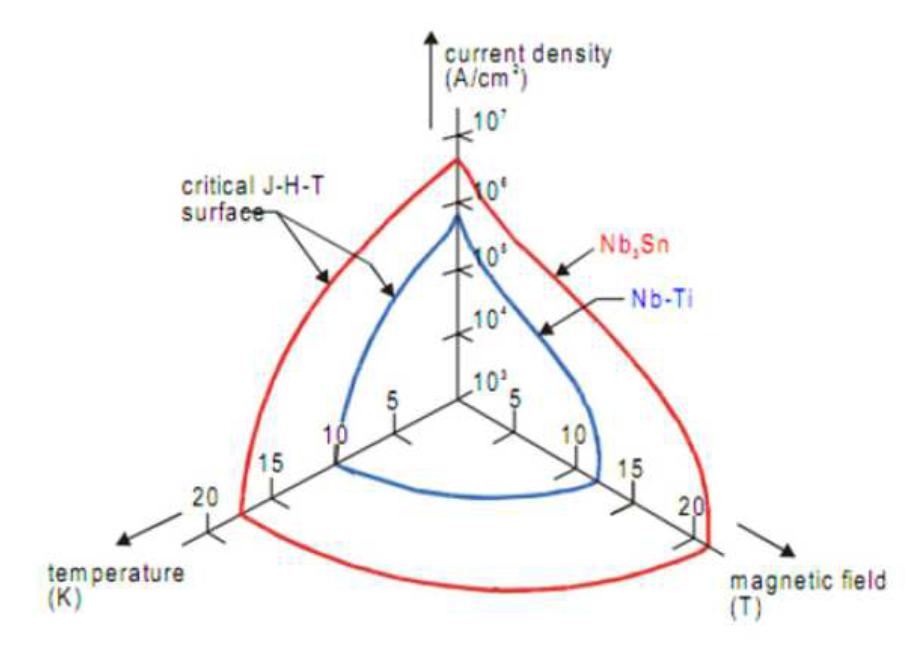
\includegraphics[width=0.49\linewidth]{figures/introduction/critical_surface_scheme.png}
\caption{Schematic of the critical surface of $\text{Nb}_\text{3}\text{Sn}$ and Nb-Ti \cite{evans_marvel_of_technology}}
\label{fig:scheme_critical_surface}
\end{figure}

\subsection{Quench Problem}

    \subsubsection{Copper Resistivity}
    Copper residual resistivity ratio according to NIST: 
    \begin{equation}
    RRR = \frac{\rho(T=273~\text{K}, B=0~\text{T})}{\rho(T=4~\text{K}, B=0~\text{T})}
    \end{equation}
    
    \subsubsection{Critical Parameters for Superconductivity}
    Critical current:
    \begin{equation}
        I_\text{c}(T) = I \frac{T-T_\text{cs}}{T_\text{c}-T_\text{cs}}
    \end{equation}
    \\
    Critical temperature:
    \begin{equation}
        T_\text{c}(B) = 9.2 \cdot [1- \frac{B}{14.5}]^{0.59}~\text{for}~B~<~10~\text{T}
    \end{equation}
    \\
    Critical magnetic field: 
    \begin{equation}
        B_\text{c2}(T) = B_\text{c2}(T=0) \cdot [1-(\frac{T}{T_\text{c}(B=0)})^{n}],
    \end{equation}
    where
    $B_\text{c2}(T=0)=14.5~\text{T}$, $T_\text{c}(B=0)=9.2~\text{K}$, $n=1.7$.

    \subsubsection{Current Flow in Copper Matrix}
    
    Current sharing temperature: 
    \begin{equation}
        T_\text{cs} = T_\text{c} (1 - \frac{I}{\text{c}_1 + \text{c}_2 B }),
    \end{equation}
    where $\text{c}_1=3449~\text{A}$ and $\text{c}_2=-257~\text{AT}^{-1}$
    \\
    Current in copper matrix: 
    \begin{equation}
        \left\{ \begin{array}{lll}
        I_\text{Cu} = 0 & \text{for}~T < T_\text{cs} \\ \\
        I_\text{Cu} = I - I_\text{c} & \text{for}~T_\text{cs} \leq T<T_\text{c}  \\ \\
        I_\text{Cu} = I & \text{for}~T_\text{cs} \leq T
        \end{array} \right.
    \end{equation}
    \\
    Joule heating: 
    \begin{equation}
        \left\{ \begin{array}{lll}
        q_\text{Joule} = 0 & \text{for}~T < T_\text{cs} \\ \\
        q_\text{Joule} = \rho_\text{Cu}(T, B) \frac{(I-I_\text{c})^2}{{\text{a}_\text{Cu}}^2}& \text{for}~T_\text{cs} \leq T<T_\text{c}  \\ \\
        q_\text{Joule} = \rho_\text{Cu}(T, B) \frac{I^2}{{\text{a}_\text{Cu}}^2} & \text{for}~T_\text{cs} \leq T
        \end{array} \right.
    \end{equation}

    \begin{figure}[ht!]
    \centering
    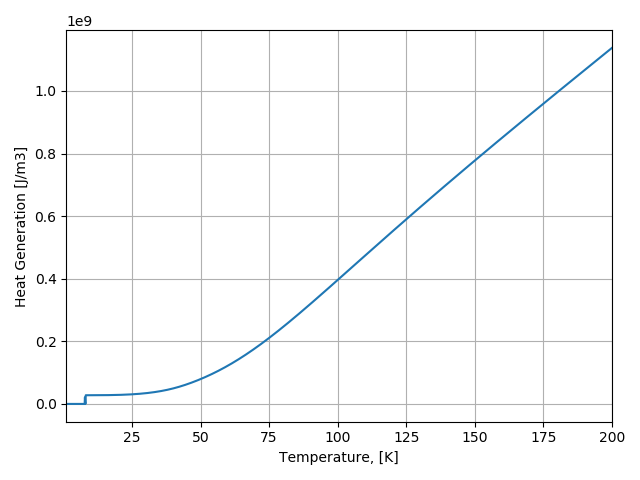
\includegraphics[width=0.49\linewidth]{figures/skew_quad_bcs/magnetic_field_mapping/Heat_Generation_Curve_B_3.png}
    \caption{Heat Generation Curve as a function of temperature for B=3 T}
    \label{fig:H_gen_curve}
    \end{figure}
    
\subsection{Accelerator Magnets}
What type of magnets can we find? \\
How are they protected? \\
Passive and active protections \\ 
Self-protectability

\subsection{Analyses in Superconductors}

\subsection{Numerical Analyses}

Heat conduction equation: 
\begin{equation}
    \frac{\partial}{\partial x}[k(B) \frac{\partial T}{\partial x}] + q_v = \rho c_p \frac{\partial T}{\partial t}
\end{equation}

\subsection{Thermal Numerical Analyses}

To write in introduction: 
Wilson: \\
- point disturbances (page 74) \\
- minimum propagating zone (MPZ) (same page - up to 80 something...)

% AIM THESIS
\clearpage \thispagestyle{empty}
\section{Aim of Thesis}

\subsection{Research Aim and Objectives}

Solving temperature distribution in a superconducting magnet in 3D where quench is considered is a challenging task. The~reasons standing behind this are twofold: $(i)$~nonlinear material properties at cryogenic temperatures; $(ii)$~high temperature gradients at the quench front. When a numerical solver deals with the problem characterised as follows, it decreases its time step in order to reach convergence. It also requires a finer mesh to represent the steep temperature change at the quench front. Both implications make the simulation computationally demanding. A good example of the level of non-linearities at cryogenic temperatures is thermal conductivity of copper. Its value changes from 250 to 1700 $\frac{\text{W}}{\text{m K}}$ at $T \in (1.9, 20)~\text{K}$ for $B=3~\text{T}$ according to NIST\footnote{NIST -- National Institute of Standards and Technology} \cite[p.~9-13]{material_properties_roxie}.

Since the 3D thermal models are computationally demanding, they are not suitable for use in magnet design which is an intrinsically iterative process. In this thesis, there are two scientific questions asked:

\begin{enumerate}
\item Can a multidimensional thermal analysis in superconducting accelerator magnets be more efficient computationally?
\item  Can such an optimised modelling for superconducting accelerator magnets be conducted in ANSYS which is nowadays one of the most widespread commercial tools for FEM numerical simulations on the market?
\end{enumerate}

One can ask a question whether there exist methods for approximating the quench problem which would allow for obtaining quick and reliable solution. If the quench position in time was known a priori and estimated beforehand, the numerical solver would solve the temperature distribution faster over the coil domain. Such an approach has been inspired by ITER's Magnet Division approach to quench modelling of toroidal superconducting magnets in fusion applications~\cite{iter_presentation_qualified_analysis, iter_fault_case_study}. In this thesis, this method, called quench velocity modelling, is applied for the case of accelerator superconducting magnets. 


\subsection{Structure of the Thesis}

The thesis is divided as follows. Chapter~\ref{chapter: introduction} is a general introduction to the quench analysis in superconducting magnets that allows the reader to smoothly acquaint with the problematics of the thesis. Chapter~\ref{chapter: aim_thesis} depicts the main objectives of this work. Since at TE-MPE-PE section\footnote{TE-MPE-PE is an abbreviation for Performance Evaluation Section belonging to Machine Protection and Electrical Integrity Group being part of Technology Department at CERN.}, COMSOL is used as the standard software for solving thermal quench problems, in Chapter~\ref{chapter: 1d_quench_propagation_modelling}, 1D quench propagation is solved in both ANSYS and COMSOL to cross-check the results. The analyses of a 1D strand are conducted with and without an insulation layer and resin. Chapter~\ref{chapter:quench_velocity_modelling} explains in detail the quench velocity-based approach to solve multi-dimensional thermal problems in superconducting magnets.
Chapter~\ref{chapter:algorithms} describes the algorithms created to perform a multi-dimensional thermal analysis. Chapter~\ref{chapter:python_implementation} deals with how the foregoing algorithms are implemented in the simulations through Python scripts and as well as in ANSYS APDL scripts. Chapter~\ref{chapter:quench_velocity_benchmarking} compares the quench velocity-based approach with standard analyses performed in Chapter~\ref{chapter: 1d_quench_propagation_modelling}. In Chapter~\ref{chapter:skew_quadrupole_quench_detection_analysis}, the quench velocity-based approach is applied to solve a multi-dimensional thermal problem of a skew quadrupole, being one of the high-order corrector magnets for the High-Luminosity LHC upgrade. The analysis is performed: $(i)$ at constant current to simulate the quench propagation until the quench is detected, $(ii)$ at varying current during the magnet discharge after the quench detection. The simulation results are compared with available measurements. Chapter~\ref{chapter:research_questions_discussions} summarises the covered topics as well provides an answer to the research questions proposed in this thesis.



% 1D QUENCH PROPAGATION MODELLING 
\clearpage
\section{1D Quench Propagation Modelling}
\label{section: 1d_quench_propagation_modelling}

In this section, 1D analysis of a single strand is conducted in ANSYS and COMSOL software. There are two cases considered: 

\begin{itemize}
    \item 1D strand analysis without insulation layer,
    \item 1D strand analysis with an external insulation layer.
\end{itemize}

For both cases, the mesh density study is conducted. In the given analyses, there are several assumptions made: 

\begin{itemize}
    \item There is no helium cooling.
    \item Temperature in the winding's cross-sectional area is uniform.
    \item When the insulation layer is considered, the longitudinal heat transfer inside the insulation is negligible with respect to the transversal one.
\end{itemize}

The \nth{2} assumption allows one to consider this problem as a 1D longitudinal heat propagation. When the insulation layer is also simulated within the \nth{3} assumption, the analysis becomes a 1D+1D heat propagation problem. It will be further explained in section \ref{subsection: 1D_quench_propagation_with_insulation}.

\subsection{Geometry}
\label{subsection: 1d_quench_propagation_geometry}

In this thesis, all the simulations are based on the geometry of a skew quadrupole which belongs to the group of high-order corrector magnets designed for the High-Luminosity LHC upgrade. The skew quadrupole is developed by the LASA laboratory of INFN-Milano. Its geometry is presented in Fig. \ref{fig:Skew_quad_geometry}. Each coil of the skew quadrupole (marked in red in the left picture) is fully impregnated and positioned in two mechanical supports (marked in grey). The entire magnet is surrounded by an iron yoke (marked in blue). One coil of a magnet out of four in total is presented in the right picture.

\begin{figure}[H]
    \centering
    \begin{tikzpicture}
    \node at (0,0) {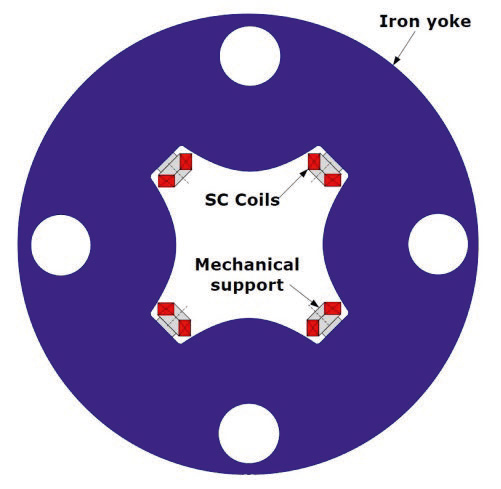
\includegraphics[width=0.3\linewidth]{sections/1D_quench_modelling/figures/geometry/Quadrupole_Cross_Section.png}};
    \node at (5,0) {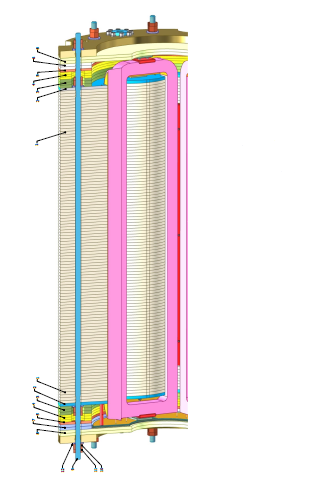
\includegraphics[width=0.225\linewidth]{sections/1D_quench_modelling/figures/geometry/SkewQuad3D.png}};
    \end{tikzpicture}
     \caption{Left: cross-section of the skew quadrupole~\cite[p.~103-105]{hl_lhc_tech_design_report_v01}; right: one coil of the skew quadrupole~\cite{marco_prioli_mails}.}
    \label{fig:Skew_quad_geometry}
\end{figure}

As presented in Fig.~\ref{fig: 1d_strand_geometry}, the coil consists of a composite strand marked in yellow made of Nb-Ti and a copper stabiliser. The strand is fully insulated with an S2-glass material marked in red. The cable is wound 754 times to form a coil with the total length of 812~m~\cite{samuele_mariotto_mails}. After the winding process, the coil is impregnated with an epoxy resin CTD-101K marked in blue in Fig.~\ref{fig: 1d_strand_geometry}. The Rutherford cable is not applied in high-order corrector magnets. In the remainder of the thesis, the term "cable" is restricted to the composite strand made of a superconductor and a copper stabiliser including an external insulation layer and, optionally, a resin filler. The bare cable and winding are referred to as "strand". The one-dimensional coordinate system $\bar x$ in Fig.~\ref{fig: 1d_strand_geometry} represents the longitudinal direction of the strand. The 1D geometry is based on geometrical parameters of a single strand of the skew quadrupole whose simulations are further described in the next section. 

\begin{figure}[H]
    \centering
    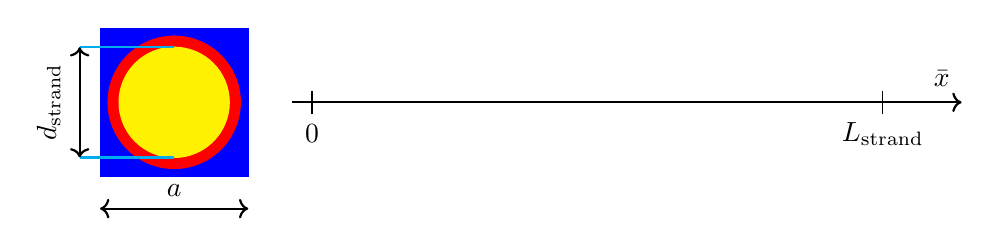
\begin{tikzpicture}[scale = 1]
        \filldraw[blue] (-0.941,-0.941) rectangle (0.941,0.941);
        \filldraw[red] (0,0) circle (0.7+0.07*2);
        \filldraw[yellow] (0,0) circle (0.7);
        \draw[thick, cyan] (-0.8*1.5,0.7) -- (0,0.7);
        \draw[thick, cyan] (-0.8*1.5,-0.7) -- (0,-0.7);
        \draw[black, thick, <->] (-0.75*1.6,0.7) -- (-0.75*1.6,-0.7);
        \node[scale = 1, rotate=90] at (-1.1*1.45, 0) {$d_\text{strand}$};
        \draw[thick,<->] (-0.941,-0.9*1.5) -- (0.941,-0.9*1.5);
        \node[scale = 1] at (0, -0.7*1.6) {$a$};
        \draw[thick,->] (1.5,0) -- (10.0,0);
        \draw[thin] (1.75,-0.15) -- (1.75,0.15);
        \draw[thin] (9,-0.15) -- (9,0.15);
        
        \node[scale = 1] at (9.75, 0.3) {$\bar x$};
        \node[scale = 1] at (9, -0.4) {$L_\text{strand}$};
        \node[scale = 1] at (1.75, -0.4) {0};
        
    \end{tikzpicture}
    \caption{1D strand geometry.}
    \label{fig: 1d_strand_geometry}
\end{figure}

The parameters of the skew quadrupole presented in Table \ref{table:skew_quad_params_table_basic} do not change in the remainder of the thesis. The last two: $(i)$ residual resistivity ratio, RRR, $(ii)$ copper-to-superconductor ratio, $r_\text{Cu/sc}$ are obtained from the measurements of the prototype magnet performed at INFN.~\cite{marco_prioli_mails}

\begin{table}[H]
    \caption{Geometrical parameters of the skew quadrupole \cite{hl_lhc_tech_design_report_v01, marco_prioli_mails}.} 
    \vspace{-1.em} 
    \fontsize{10}{10}
    \selectfont 
    \renewcommand{\arraystretch}{1.5}
    \begin{center}
    \begin{tabular}{ ccc }  
    \hline
    parameter & value & unit \\
    \hline
    $d_\text{strand}$ & 0.7 & [mm] \\
    $a$ & 0.941 & [mm] \\
    $r_\text{Cu/sc}$ & 2.2 & [-] \\
    RRR & 193 & [-] \\  
    \hline 
    \end{tabular}
    \end{center}  
     \label{table:skew_quad_params_table_basic} 
 \end{table}


\subsection{1D Analysis without Insulation}
\label{subsection: 1D_quench_propagation_no_insulation}

\subsection{Geometry, Material Properties and Mesh}

Since copper and Nb-Ti are characterised by a~different volumetric heat capacity, the total volumetric heat capacity of a strand is given by

\begin{equation}
    c_\text{v, strand} = f_\text{Cu} ~ c_\text{v, Cu}(T) + f_\text{Nb-Ti} ~ c_\text{v, Nb-Ti}(T,B),
    \label{eqn: cv_equiv}
\end{equation}
where $c_\text{v, Cu}$ -- volumetric heat capacity of copper as a function of temperature, $c_\text{v, Nb-Ti}$ -- volumetric heat capacity of Nb-Ti as a function of temperature and magnetic field, $f_\text{Cu}$ -- volumetric fraction of copper, $f_\text{Nb-Ti}$ -- volumetric fraction of Nb-Ti. The~volumetric heat capacity of the composite strand for a given value of $B$ and $r_\text{Cu/sc}$ is shown in Fig. \ref{fig:eq_wind_cp}.

\begin{figure}[H]
\centering
    \begin{tikzpicture}
        \begin{axis}[
          no markers,
          width=0.7\linewidth, 
          height = 4.5cm,
          xlabel={$T,~\text{K}$},
          ylabel={$c_\text{v, strand},~\frac{\text{J}}{\text{m}^3 \cdot \text{K}}$},
          xmin=0.0,
          ymin=0.0,
          xmax=300.0
          ]
          \addplot table[x=temperature,y=cv_equiv,col sep=comma] {sections/1D_quench_modelling/figures/other/cv_equivalent.csv}; 
        \end{axis}
    \end{tikzpicture}
    \caption{Strand volumetric heat capacity as a function of temperature for $B=2~\text{T}$ and $r_\text{Cu/sc}=2.2$.}
    \label{fig:eq_wind_cp}
\end{figure}

According to~\cite[p.~46]{material_props_for_heat_transfer_modelling_in_nb3sn_magnets}, the thermal conductivity of Nb-Ti changes from 1 to 9~$\frac{\text{W}}{\text{m K}}$ in the temperature range of $T \in (20, 200)~\text{K}$. At temperatures below 20~K, the thermal conductivity of Nb-Ti is lower than~$1~\frac{\text{W}}{\text{m K}}$. By comparing the thermal conductivity of Nb-Ti and copper, whose thermal conductivity is presented in Appendix~\ref{subsection:copper_thermal_conductivity}, one can conclude that the thermal conductivity of Nb-Ti is negligible and only the part of copper contributes to the longitudinal heat propagation, as 
\begin{equation}
    k_\text{strand} = f_\text{Cu} ~ k_\text{Cu} + f_\text{Nb-Ti} ~ k_\text{Nb-Ti} \approx  f_\text{Cu} ~ k_\text{Cu},
    \label{eqn: k_equiv}
\end{equation}
where $k_\text{strand}$ -- thermal conductivity of a strand, $k_\text{Cu}$ -- thermal conductivity of copper, $k_\text{Nb-Ti}$ -- thermal conductivity of Nb-Ti. It is important to highlight that only in Chapter~\ref{chapter: 1d_quench_propagation_modelling}, the thermal conductivity of copper is calculated according to the Wiedemann-Franz formula, as
\begin{equation}
    k_\text{Cu} = 2.45 \cdot 10^{-8} ~ \frac{T}{\rho_\text{Cu}}.
    \label{eqn: k_cu_wiedemann_franz}
\end{equation}
Wiedeman-Franz formula is used for the sake of comparison of the results with COMSOL in which only such material property is available. In the remainder of the thesis, the thermal conductivity of copper and all other material properties are calculated according to the fits provided by NIST, as described in Appendix~\ref{appendix_material_properties_description}. 

In ANSYS, the element LINK33 is used to the 1D quench propagation. It is a uniaxial 2-node linear element with the ability to conduct heat between its nodes suitable for steady-state and transient analyses~\cite{ansys_element_manual}. Unlike ANSYS, COMSOL does not use explicit element types to define physical equations in a domain. Instead, one has to choose from a list of available physics modules, in this case thermal physics. Therefore, the algebraic physical equations related to heat conduction in COMSOL are applied to the nodes belonging to the composite strand. In both tools, a uniformly distributed mesh is used with mesh size equal to 0.1 mm. The mesh size is based on~\cite[p.~40]{paudel_thesis} in which it is recommended to discretise the domain in the scale less than or equal to 1~mm for an adiabatic analysis of a 1D quench propagation.

\subsection{Initial and Boundary Conditions, and Solver Settings}

Over the entire length of the strand, the power density is applied according to~(\ref{eqn: p_dens_equiv}). In addition, a Gaussian profile of the initial temperature is assumed according to 
\begin{equation}
    T(x) = T_\text{init} + (T_\text{max} - T_\text{init}) ~ e^{-(\frac{x}{\alpha})^2},
    \label{eqn: gaussian_temp_ic}
\end{equation}
where $T(x)$ -- temperature profile along $x$-axis, $T_\text{init}$ -- initial bath temperature of a strand, $T_\text{max}$ -- the maximum temperature of the Gaussian profile, $\alpha$ -- shape parameter of the Gaussian profile proportional to the standard deviation. The input parameters corresponding to the Gaussian profile, initial transport current, and initially quenched zone are depicted in Table~\ref{table: 1d_quench_propagation_analysis_init_temp_input_parameters}. 

\begin{table}[H]
    \caption{Input parameters for the 1D analysis.} 
    \vspace{-1.em} 
    \fontsize{10}{10}
    \selectfont 
    \renewcommand{\arraystretch}{1.5}
    \begin{center}
        \begin{tabular}{ ccc }  
        \hline
        parameter & value & unit \\
        \hline
        $I$ & 100 & [A] \\
        $B$ & 2 & [T] \\
        $T_\text{init}$ & 1.9 & [K] \\
        $T_\text{max}$ & 20.0 & [K] \\
        $T_\text{c}$ & 8.429 & [K] \\
        $L_\text{quench, init}$ & 0.1 & [m] \\ 
        $\alpha$ & 0.223 & [m] \\   
        \hline 
        \end{tabular}
    \end{center}  
     \label{table: 1d_quench_propagation_analysis_init_temp_input_parameters} 
 \end{table}

The initially quenched zone is equal to $L_\text{quench, init}= 0.1~\text{m}$ when symmetry is not taken into consideration. It~means that at $x=0.05~\text{m}$, the strand is at the critical temperature for the given magnetic field strength. The shape parameter, \textalpha~in (\ref{eqn: gaussian_temp_ic}) is calculated accordingly. The critical temperature $T_\text{c}$ is calculated as in (\ref{eqn:critical_temperature_appendix}) in Appendix~\ref{appendix:nbti_material_properties}. A symmetry condition is applied at the position $x=0~\text{m}$. Thus, a one metre-long strand represents a half of the analysed domain, as presented in Fig. \ref{fig: init_gauss_temp_distr}.

\begin{figure}[H]
\centering
    \begin{tikzpicture}
        \begin{axis}[
          no markers,
          width=0.7\linewidth, 
          height = 4.5cm,
          xlabel={$L_\text{strand},~\text{m}$},
          ylabel={$T,~\text{K}$},
          xmin=0.0,
          ymin=0.0,
          xmax=1.0
          ]
          \addplot table[x=posx,y=temperature,col sep=comma] {sections/1D_quench_modelling/figures/other/gaus_init_distr.csv}; 
        \end{axis}
    \end{tikzpicture}
    \caption{Initial Gaussian temperature distribution.}
    \label{fig: init_gauss_temp_distr}
\end{figure}

The solution in both ANSYS and COMSOL are obtained with a strict time stepping, i.e. the time step during the solution is fixed. The input parameters related to the time stepping algorithm and the total simulation time are presented in Table \ref{table: 1d_quench_propagation_analysis_time_stepping_input_parameters}. ANSYS uses a default sparse solver with an automatic solution control setting. In COMSOL, the Multifrontal Massively Parallel Sparse Direct Solver (MUMPS) is applied. Both tools use direct solvers with an implicit Backward Euler time stepping method~\cite{comsol_webpage, ansys_command_reference}. In a time-dependent domain, default values for time stepping convergence are applied in both ANSYS and COMSOL. The geometry is built based on the \nth{1} order elements in each tool.

\begin{table}[H]
    \caption{Analysis time stepping input parameters.} 
    \vspace{-1.em} 
    \fontsize{10}{10}
    \selectfont 
    \renewcommand{\arraystretch}{1.5}
    \begin{center}
        \begin{tabular}{ ccc }  
        \hline
        parameter & value & unit \\
        \hline
        $t_\text{total}$ & $10^{-1}$ & [s] \\   
        $t_\text{step, max}$ & $10^{-4}$ & [s] \\   
        \hline 
        \end{tabular}
    \end{center}  
     \label{table: 1d_quench_propagation_analysis_time_stepping_input_parameters} 
 \end{table}

\subsection{Results}
\label{subsubsection:1d_quench_propagation_analysis_results_no_insulation}

The temperature distribution profiles are compared at three time steps $t=\{0.03, 0.06, 0.1\}$~s, as presented in Fig.~\ref{fig: 1d_no_insulation_temp_along_strand_comparison}. One can conclude that the initial heat pulse is sufficient to initiate quench. In fact, relatively high thermal conductivity and low heat capacity of the strand allow for a longitudinal quench propagation. At each time window, the hot-spot is placed at $x=0~\text{m}$. In general, COMSOL predicts faster quench propagation.

\begin{figure}[H]
\centering
    \begin{tikzpicture}
        \begin{axis}[
          no markers,
          width=0.7\linewidth, 
          height = 5.0cm,
          xlabel={$\bar{x},~\text{m}$},
          ylabel={$T,~\text{K}$},
          xmin=0.0,
          ymin=0.0,
          xmax=1.0,
          legend pos=outer north east
          ]
        %   Initial temperature curve
          \addplot[smooth, black] table[x=posx,y=t_0_0_ans,col sep=comma] {sections/1D_quench_modelling/figures/results_no_insulation/Temp_tstep_10ms_1e4elems_f2_2.csv};
          
        %   COMSOL plots
          \addplot[smooth, red] table[x=posx,y=t_0_03_com,col sep=comma] {sections/1D_quench_modelling/figures/results_no_insulation/Temp_tstep_10ms_1e4elems_f2_2.csv};
          \addplot[smooth, red] table[x=posx,y=t_0_06_com,col sep=comma] {sections/1D_quench_modelling/figures/results_no_insulation/Temp_tstep_10ms_1e4elems_f2_2.csv};
          \addplot[smooth, red] table[x=posx,y=t_0_1_com,col sep=comma] {sections/1D_quench_modelling/figures/results_no_insulation/Temp_tstep_10ms_1e4elems_f2_2.csv};

        %   ANSYS plots
          \addplot[smooth, blue] table[x=posx,y=t_0_03_ans,col sep=comma] {sections/1D_quench_modelling/figures/results_no_insulation/Temp_tstep_10ms_1e4elems_f2_2.csv};
          \addplot[smooth, blue] table[x=posx,y=t_0_06_ans,col sep=comma] {sections/1D_quench_modelling/figures/results_no_insulation/Temp_tstep_10ms_1e4elems_f2_2.csv};
          \addplot[smooth, blue] table[x=posx,y=t_0_1_ans,col sep=comma] {sections/1D_quench_modelling/figures/results_no_insulation/Temp_tstep_10ms_1e4elems_f2_2.csv};
          
          \legend{
          $T_\text{init}$,
          COMSOL,,,
          ANSYS
          }
        \end{axis}
        
        \draw[black, thick, ->] (2,3) -- (3,3);
        \node[scale = 1] at (3.8, 3) {$\vec{v}_\text{quench}$};   
        
    \end{tikzpicture}
    \caption{Temperature distribution calculated in COMSOL and ANSYS for three time steps: $t=\{0.03, 0.06, 0.1\}$~s with a specified direction of the quench propagation, $\vec{v}_\text{quench}$.}
    \label{fig: 1d_no_insulation_temp_along_strand_comparison}
\end{figure}

The quench velocity is calculated by comparing the position of the quench front at $t=0.06~\text{s}$ and $t=0.1~\text{s}$, assuming that at this moment, the quench propagation velocity reaches a steady-state value. The relative error is calculated as
\begin{equation}
    E_\text{r} = \frac{r_\text{ANSYS}-r_\text{COMSOL}}{r_\text{COMSOL}}~100\%,
    \label{eqn:relative_error_comsol_ansys_benchmarking}
\end{equation}
where $r_\text{ANSYS}$ -- a given result from ANSYS, $r_\text{COMSOL}$ -- a given result from COMSOL. The~relative error is estimated for:

\begin{itemize}
    \item quench velocity, as presented in Table \ref{table: 1d_no_insulation_v_quench_comparison},
    \item temperature along the strand length at $t=0.1~\text{s}$, as presented in Fig. \ref{fig: ans_comsol_comparison_rel_error_temp_f_2_2}.
\end{itemize}

\begin{table}[H]
    \caption{Quench velocity comparison between COMSOL and ANSYS.} 
    \vspace{-1.em} 
    \fontsize{10}{10}
    \selectfont 
    \renewcommand{\arraystretch}{1.5}
    \begin{center}
        \begin{tabular}{ ccc }  
        \hline
        parameter & value & unit \\
        \hline
        $v_\text{quench, COMSOL}$ & 7.075 & [m/s] \\
        $v_\text{quench, ANSYS}$ & 6.968 & [m/s] \\
        $E_\text{r}$ & -1.519 & [\%] \\
        \hline 
        \end{tabular}
    \end{center}  
     \label{table: 1d_no_insulation_v_quench_comparison} 
 \end{table}

\begin{figure}[H]
\centering
    \begin{tikzpicture}
        \begin{axis}[
          width=0.7\linewidth, 
          height = 4.5cm,
          xlabel={$\bar{x},~\text{m}$},
          ylabel={$E_\text{r}$, \%},
          xmin=0.0,
          xmax=1.0
          ]
          \addplot[blue, mark=*] table[x=posx,y=error_0_1,col sep=comma] {sections/1D_quench_modelling/figures/results_no_insulation/Temp_tstep_10ms_1e4elems_f2_2_error.csv};
        \end{axis}
    \end{tikzpicture}
    \caption{Relative error along the strand with respect to the temperature distribution for $t=0.1~\text{s}$.}
    \label{fig: ans_comsol_comparison_rel_error_temp_f_2_2}
\end{figure}

The difference in the hot-spot temperature at $x=0~\text{m}$ does not exceed 0.06 \%. The quench velocity in ANSYS is lower than the one in COMSOL by less than 2~\% which results in the increase of the relative error corresponding to the nodal temperature distribution up to 20~\% close to the quench front at $t=0.1~\text{s}$.

\subsection{1D Analysis with Insulation}
\label{subsection: 1D_quench_propagation_with_insulation}

\subsection{Geometry, Material Properties and Mesh}

Because of the lack of data about thermal material properties of D10 and S2-glass at cryogenic temperatures, it is assumed in this thesis that the region outside of the composite strand is homogenised and represented by G10. G10 is a material widely known and applied in the superconducting magnet design community. Its material properties are presented in Appendix~\ref{appendix_material_properties_description}.

The longitudinal heat transfer inside the insulation is assumed to be negligible with respect to the transversal one. In order to prove the validity of this assumption, the thermal diffusivity of a composite strand was compared with the one of the insulation layer, i.e. G10. The ratio of two thermal diffusivities is calculated as
\begin{equation}
    \frac{\alpha_\text{strand}}{\alpha_\text{ins}} = \frac{k_\text{strand}}{k_\text{ins}}~\frac{C_\text{v, ins}}{C_\text{v, strand}},
    \label{eqn: diffusivity_strand_to_insulation_ratio}
\end{equation}
where $\alpha_\text{strand}$ -- thermal diffusivity of a strand, $\alpha_\text{ins}$ -- thermal diffusivity of the insulation layer, $k_\text{ins}$~-- thermal conductivity of the insulation layer, $C_\text{v, ins}$ -- volumetric heat capacity of the insulation layer. 

As presented in Fig. \ref{fig:diffusivity_strand_to_insulation_ratio}, the longitudinal thermal diffusivity of the strand is in the range of 2 and 5 orders of magnitude higher than the one of the insulation layer. The ratio stabilises at $T>100~\text{K}$ and is approximately equal to 100. Because of such a high difference in thermal diffusivity of the strand and the insulation, it is assumed that the longitudinal thermal diffusivity of the insulation is negligible. Therefore, the insulation is modelled as 1D elements placed transversely to the strand elements.

\begin{figure}[H]
\centering
    \begin{tikzpicture}
        \begin{axis}[
          no markers,
          width=0.7\linewidth, 
          height = 4.5cm,
          ymode=log,
          xmode=log,
          xlabel={$T,~\text{K}$},
          ylabel={$\frac{\alpha_\text{strand}}{\alpha_\text{ins}}$},
          xmax=300.0
          ]
          \addplot table[x=temperature,y=diffusivity_ratio,col sep=comma] {sections/1D_quench_modelling/figures/other/diffusivity_strand_insul_ratio.csv}; 
        \end{axis}
    \end{tikzpicture}
    \caption{Strand equivalent thermal diffusivity to insulation thermal diffusivity ratio for $B=2~\text{T}$ and $r_\text{Cu/Nb-Ti}$.}
    \label{fig:diffusivity_strand_to_insulation_ratio}
\end{figure}

With specified assumptions, the 3D strand domain can be transformed into a 1D+1D domain including the strand as well as the insulation, as presented in Fig. \ref{fig: 1d_strand_geometry_with_insulation}. Each of the 1D insulation domains orthogonal to the 1D strand is characterised by an equivalent length, $L_\text{ins}$ and a conduction area, $A_\text{ins, cond}$. Both parameters should be calculated to obtain the total volume of the insulation equal for two cases: 1D+1D and 3D. It allows for obtaining the same volumetric heat capacity for both cases.

\begin{figure}[H]
    \centering
    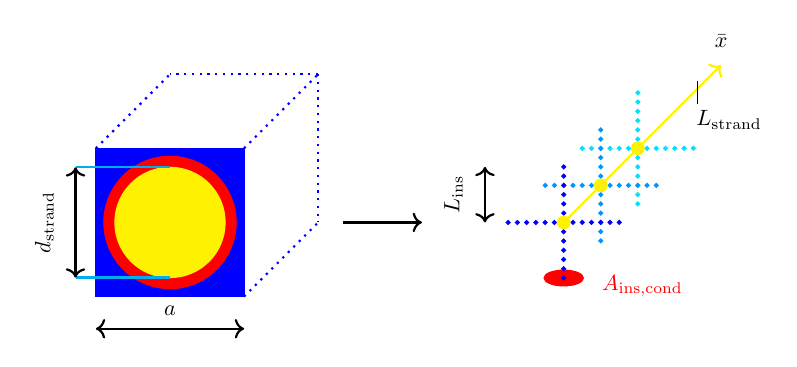
\begin{tikzpicture}[scale = 1]
        \filldraw[blue] (-0.941,-0.941) rectangle (0.941,0.941);
        \filldraw[red] (0,0) circle (0.7+0.07*2);
        \filldraw[yellow] (0,0) circle (0.7);
        \draw[thick, cyan] (-0.8*1.5,0.7) -- (0,0.7);
        \draw[thick, cyan] (-0.8*1.5,-0.7) -- (0,-0.7);
        \draw[black, thick, <->] (-0.75*1.6,0.7) -- (-0.75*1.6,-0.7);
        \node[scale = 0.8, rotate=90] at (-1.1*1.45, 0) {$d_\text{strand}$};
        \draw[thick,<->] (-0.941,-0.9*1.5) -- (0.941,-0.9*1.5);
        \node[scale = 0.8] at (0, -0.7*1.6) {$a$};
        \draw[thick, dotted, blue] (0.941,0.941) -- (2*0.941,2*0.941);
        \draw[thick, dotted, blue] (-0.941,0.941) -- (0,2*0.941);
        \draw[thick, dotted, blue] (0.941,-0.941) -- (2*0.941,0);
        \draw[thick, dotted, blue] (2*0.941,2*0.941) -- (2*0.941,0);
        \draw[thick, dotted, blue] (2*0.941,2*0.941) -- (0,2*0.941);
        % ellipse for insulation area
        \filldraw[red] (5.0,-5.646/8) ellipse (0.25cm and 0.1cm);
        \node[scale = 0.8, red] at (6.0, -5.646/8-0.1) {$A_\text{ins,cond}$};
        % third insulation layer
        \definecolor{blue_third_layer}{RGB}{0,225,255}
        \foreach \x in {-5.646,-4.705,...,5.646} 
            \filldraw[blue_third_layer] (5.0+2*0.4705,\x/8+2*0.4705) circle (0.025);
        \foreach \x in {-5.646,-4.705,...,5.646} 
            \filldraw[blue_third_layer] (5.0+\x/8+2*0.4705,2*0.4705) circle (0.025);
        % second insulation layer
        \definecolor{blue_second_layer}{RGB}{0,150,255}
        \foreach \x in {-5.646,-4.705,...,5.646} 
            \filldraw[blue_second_layer] (5.0+0.4705,\x/8+0.4705) circle (0.025);
        \foreach \x in {-5.646,-4.705,...,5.646} 
            \filldraw[blue_second_layer] (5.0+\x/8+0.4705,0.4705) circle (0.025);
        % first insulation layer
        \definecolor{blue_first_layer}{RGB}{0,0,255}
        \foreach \x in {-5.646,-4.705,...,5.646} 
            \filldraw[blue_first_layer] (5.0,\x/8) circle (0.025);
        \foreach \x in {-5.646,-4.705,...,5.646} 
            \filldraw[blue_first_layer] (5.0+\x/8,0) circle (0.025);
        % strand nodes
        \draw[thick, yellow, ->] (5.0,0) -- (7.0,2.0);
        \foreach \t in {0.0,0.4705,...,1.4115}
            \filldraw[yellow] (5.0+\t,\t) circle (0.08);
        \node[scale = 0.8] at (7.1, 1.3) {$L_\text{strand}$};    
        \node[scale = 0.8] at (7, 2.3) {$\bar x$};    
        \draw[thin] (6.7,1.5) -- (6.7,1.8);
        \draw[thick, black, <->] (4,0) -- (4,5.646/8);
        \node[scale = 0.8, rotate=90] at (3.6, 5.646/16) {$L_\text{ins}$}; 
        % draw arrow
        \draw[thick, black, ->] (2.2,0) -- (3.2,0);
    \end{tikzpicture}
    \caption{3-dimensional transformation of a 1D+1D strand domain in ANSYS.}
    \label{fig: 1d_strand_geometry_with_insulation}
\end{figure}

In order to define the geometric parameters for the insulation layer, one should calculate the insulation cross-sectional area as
\begin{equation}
    A_\text{ins} = a^2 - \frac{\pi d_\text{strand}^2}{4}, 
    \label{eqn:cross_sectional_area_insulation}
\end{equation}
where $a$ -- strand side, $d_\text{strand}$ -- strand diameter. Then, the average insulation perimeter is estimated as
\begin{equation}
    p_\text{avg} = \frac{4 a + \pi d_\text{strand}}{2}.
    \label{eqn:average_perimeter}
\end{equation}
By combining the formulae (\ref{eqn:cross_sectional_area_insulation}) and (\ref{eqn:average_perimeter}), one can calculate the equivalent insulation length as 
\begin{equation}
    L_\text{ins} = \frac{A_\text{ins}}{p_\text{avg}}.
    \label{eqn:equivalent_insulation_length}
\end{equation}
Calculating the equivalent insulation length in such a manner allows for using this approximation also in case when both the strand and the insulation are of the same shapes, e.g. if they are rectangles or circles. The conduction area of transverse elements is calculated as
\begin{equation}
    A_\text{ins, cond} = \frac{1}{4}~\frac{ V_\text{ins}}{L_\text{ins}}~\frac{1}{n_\text{nodes, strand}}= \frac{1}{4}~\frac{ A_\text{ins} ~ L_{winding}}{L_\text{ins}}~\frac{1}{n_\text{divisions, strand}},
    \label{eqn:equivalent_insulation_element_area}
\end{equation}
where $V_\text{ins}$ -- total insulation volume, $n_\text{divisions, strand}$ -- number of divisions applied along the 1D strand domain. One should remember that $A_\text{ins, cond}$ of the end insulation elements of an analysed geometry, where heat only flows in one longitudinal direction, should be divided by two.

\subsection{Initial and Boundary Conditions}

The strand geometry as well as the temperature initial conditions remain the same with respect to the analysis described in Section~\ref{section: 1D_quench_propagation_no_insulation}, as presented in Fig. \ref{fig: init_gauss_temp_distr} and Table \ref{table: 1d_quench_propagation_analysis_init_temp_input_parameters}. The time stepping is also applied, as presented in Table \ref{table: 1d_quench_propagation_analysis_time_stepping_input_parameters}, as well as the heat source over the strand with $I=100~\text{A}$. The additional parameters corresponding to the insulation are described in Table \ref{table: 1d_quench_propagation_geometry_parameters_with_insulation}. 

\begin{table}[H]
    \caption{Insulation input parameters.} 
    \vspace{-1.em} 
    \fontsize{10}{10}
    \selectfont 
    \renewcommand{\arraystretch}{1.5}
    \begin{center}
        \begin{tabular}{ ccc }
        \hline
        parameter & value & unit \\
        \hline
        $L_\text{ins}$ & 0.1679 & [mm] \\
        mesh size (insulation) & 28 & [\textmu m] \\
        \hline 
        \end{tabular}
    \end{center}  
     \label{table: 1d_quench_propagation_geometry_parameters_with_insulation} 
 \end{table}

Every orthogonal insulation domain consists of six elements of the same length. It is important to mention that in COMSOL, six orthogonal elements do not represent a quarter but a full cross-section. Therefore, the number of insulation elements in COMSOL is four times smaller and $A_\text{ins, cond}$ is four times larger.

\subsection{Results}

Similarly to Section \ref{subsubsection:1d_quench_propagation_analysis_results_no_insulation}, the results are compared at three time steps, as presented in Fig. \ref{fig: 1d_with_insulation_temp_along_strand_comparison}. 

\begin{figure}[H]
\centering
    \begin{tikzpicture}
        \begin{axis}[
          no markers,
          width=0.8\linewidth, 
          height = 5.0cm,
          xlabel={$L_\text{strand},~\text{m}$},
          ylabel={$T,~\text{K}$},
          xmin=0.0,
          ymin=0.0,
          xmax=1.0,
          legend pos=north east
          ]
        %   Initial temperature curve
          \addplot[smooth, black] table[x=posx,y=t_0_0_ans,col sep=comma] {sections/1D_quench_modelling/figures/results_with_insulation/10ms_1e4elemsf2_2ins_insTem_in.csv};
          
        %   COMSOL plots
          \addplot[smooth, red] table[x=posx,y=t_0_03_com,col sep=comma] {sections/1D_quench_modelling/figures/results_with_insulation/10ms_1e4elemsf2_2ins_insTem_in.csv};
          \addplot[smooth, red] table[x=posx,y=t_0_06_com,col sep=comma] {sections/1D_quench_modelling/figures/results_with_insulation/10ms_1e4elemsf2_2ins_insTem_in.csv};
          \addplot[smooth, red] table[x=posx,y=t_0_1_com,col sep=comma] {sections/1D_quench_modelling/figures/results_with_insulation/10ms_1e4elemsf2_2ins_insTem_in.csv};
        
        %   ANSYS plots
          \addplot[smooth, blue] table[x=posx,y=t_0_03_ans,col sep=comma] {sections/1D_quench_modelling/figures/results_with_insulation/10ms_1e4elemsf2_2ins_insTem_in.csv};
          \addplot[smooth, blue] table[x=posx,y=t_0_06_ans,col sep=comma] {sections/1D_quench_modelling/figures/results_with_insulation/10ms_1e4elemsf2_2ins_insTem_in.csv};
          \addplot[smooth, blue] table[x=posx,y=t_0_1_ans,col sep=comma] {sections/1D_quench_modelling/figures/results_with_insulation/10ms_1e4elemsf2_2ins_insTem_in.csv};
          
          \legend{
          $T_\text{init}$ profile,
          COMSOL,,,
          ANSYS
          }

        \end{axis}
                  
        \draw[black, thick, ->] (1,3) -- (2,3);
        \node[scale = 1] at (2.8, 3) {$\vec{v}_\text{quench}$}; 
        
    \end{tikzpicture}
    \caption{Temperature distribution calculated in COMSOL and ANSYS for three time steps: $t=\{0.03, 0.06, 0.1\}$~s with a specified direction of quench velocity, $\vec{v}_\text{quench}$.}
    \label{fig: 1d_with_insulation_temp_along_strand_comparison}
\end{figure}

The quench velocity was calculated by comparing the position of the quench front at $t=0.06~\text{s}$ and $t=0.1~\text{s}$. The relative error was calculated as in (\ref{eqn:relative_error_comsol_ansys_benchmarking}). The relative error was estimated for: 
\begin{itemize}
    \item quench velocity, as presented in Table \ref{table: 1d_with_insulation_v_quench_comparison},
    \item temperature along the strand length at $t=0.1~\text{s}$, as presented in Fig. \ref{fig: ans_comsol_comparison_f_2_2_with_insulation}.
\end{itemize}

\begin{table}[H]
    \caption{Quench velocity comparison in COMSOL and ANSYS.} 
    \vspace{-1.em} 
    \fontsize{10}{10}
    \selectfont 
    \renewcommand{\arraystretch}{1.5}
    \begin{center}
        \begin{tabular}{ ccc }  
        \hline
        parameter & value & unit \\
        \hline
        $v_\text{quench, COMSOL}$ & 2.308 & [m/s] \\
        $v_\text{quench, ANSYS}$ & 2.310 & [m/s] \\
        relative error & 0.108 & [\%] \\
        \hline 
        \end{tabular}
    \end{center}  
     \label{table: 1d_with_insulation_v_quench_comparison} 
 \end{table}

\begin{figure}[H]
\centering
    \begin{tikzpicture}
        \begin{axis}[
          width=0.7\linewidth, 
          height = 4.0cm,
          xlabel={$L_\text{strand},~\text{m}$},
          ylabel={Relative error, \%},
          xmin=0.0,
          xmax=1.0
          ]
          \addplot[blue, mark=*] table[x=posx,y=error_0_1,col sep=comma] {sections/1D_quench_modelling/figures/results_with_insulation/10ms_1e4elemsf2_2ins_insTem_in_error.csv};
        \end{axis}
    \end{tikzpicture}
    \caption{Relative error along the strand for $t=0.1~\text{s}$.}
    \label{fig: ans_comsol_comparison_f_2_2_with_insulation}
\end{figure}

The difference in quench velocity estimation in both models is less than 1\%, as presented in Table \ref{table: 1d_with_insulation_v_quench_comparison}. As shown in Fig. \ref{fig: 1d_with_insulation_temp_along_strand_comparison}, the relative error oscillates in the range of +2\% at the hot spot to -2\% at the quench front. It means that ANSYS overestimates the hot spot temperature and underestimates it at the quench front with respect to COMSOL.



\subsection{Conclusion}
\label{subsection: 1D_quench_propagation_conclusions}

Both simulation environments show the similar results when it comes to the problem of 1D quench thermal propagation at cryogenic temperatures. The relative error of different parameters for two software oscillated in the range of 2\%. In every analysis, a relatively dense mesh was applied of 10 nodes/mm. In  \cite{paudel_thesis}, it is recommended to discretise the domain in the scale less than or equal to a millimetre when an adiabatic analysis is conducted. 
With 10 times less dense mesh, all the analyses with insulation and without showed less than 0.5\% of a relative error. 

As concluded, in order to solve a one-metre domain, at least 1000 elements should be applied. At this point, it is interesting to estimate the scale of the thermal problem to be solved for 3-dimensional magnet geometries in which the cable length of all windings together can reach several hundreds of metres. By adding to this the influence of insulation and material non-linearities, the computing time of such analyses will easily reach at least a couple of days. Therefore, a numerical method aiming at reducing this nodal domain is strongly desired.

 
% QUENCH VELOCITY MODELLING
\clearpage
\section{Quench Velocity Modelling}
\label{section:quench_velocity_modelling}

\subsection{Concept}
\label{subsection:quench_velocity_concept}

When quench propagates, the point at which the cable transforms from superconducting to normal state moves forward with time, as shown in Fig. \ref{fig:modelling_approach}. This point remains at critical temperature, $T_\text{c}$ for a given magnetic field strength. Its rate of position change in time is described as quench velocity. Depending on electro-magneto-thermal conditions at which quench occurs, quench velocity can remain constant or change in time. 

\begin{figure}[H]
\centering
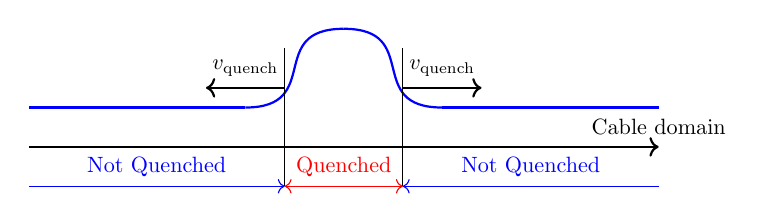
\begin{tikzpicture}[scale = 1]
\draw [thick, ->] (0.0,0.0) -- (8.0,0);

\draw [thick, blue] (0.0,0.5) -- (2.75,0.5);
\draw [thick, blue] (5.25,0.5) -- (8.0,0.5);

\draw [thick, blue] (2.75,0.5) .. controls +(0:1cm) and +(180:1cm) .. (4.0,1.5);
\draw [thick, blue] (4.0,1.5) .. controls +(0:1cm) and +(180:1cm) .. (5.25,0.5);

\draw [thin] (3.25,-0.5) -- (3.25,1.25);
\draw [thin] (4.75,-0.5) -- (4.75,1.25);

\draw [thick, ->] (4.75,0.75) -- (5.75,0.75);
\draw [thick, ->] (3.25,0.75) -- (2.25,0.75);

\draw [thin, red, <->] (3.25,-0.5) -- (4.75,-0.5);
\draw [thin, blue, ->] (0.0,-0.5) -- (3.25,-0.5);
\draw [thin, blue, <-] (4.75,-0.5) -- (8.0,-0.5);

\node[scale = 0.8] [color = red] at (4.0,-0.25) {Quenched};
\node[scale = 0.8] [color = blue] at (1.625,-0.25) {Not Quenched};
\node[scale = 0.8] [color = blue] at (6.375,-0.25) {Not Quenched};

\node[scale = 0.8] at (5.25,1.0) {$v_\text{quench}$};
\node[scale = 0.8] at (2.75,1.0) {$v_\text{quench}$};
\node[scale = 0.8] at (8.0,+0.25) {Cable domain};

\end{tikzpicture}
\caption{Quench velocity approach.}
\label{fig:modelling_approach}
\end{figure}

Quench velocity can be approximated with analytic formulas. They are usually a function of current density, material properties of the winding and temperature gradient around the quench front. The quench velocity in ITER applications is mainly estimated based on~\cite{MIT_phd_thesis}. For superconducting accelerator magnets, Wilson's formula is more applicable if cooling with helium is not considered \cite[p.~206]{wilson1987superconducting}, as described below
\begin{equation}
    v_\text{quench}=\frac{J}{\gamma C}\sqrt{\frac{\rho k}{T_\text{s}-T_\text{0}}},
    \label{eqn:Wilson_quench_velocity_formula}
\end{equation}
where $T_\text{s}$ -- critical temperature,
$T_\text{0}$ -- coolant temperature,
$\rho$ -- electrical resistivity averaged over the conductor volume,
$J$ -- current density averaged over the conductor volume,
$k$ -- thermal conductivity averaged over the conductor unit cell,
$C$ -- volumetric heat capacity averaged over the conductor unit cell,
$\gamma$ -- conductor density.

\subsection{Problematics}
\label{subsection:quench_velocity_problematics}

When a nonlinear situation is encountered in solving the heat conduction equation, the problem of this kind is handled by means of iteration. It means that the problem is linearised and the solver searches for the temperature distribution over the domain until the change of temperature between the steps will converge to a desirably low value. Due to high material non-linearities at cryogenic temperatures, in order to accurately solve the temperature distribution in the entire region of the cable, one should refine mesh and/or decrease the simulation time step (up to the order of a $\upmu$s).

Fig. \ref{fig:modelling_approach} presents an approximated temperature distribution over a discretised 1D thermal domain. The quenched and non-quenched regions in a superconducting cable have different but relatively uniform temperature distributions except for the regions close to the quench front. Therefore, the mesh density relatively far from the quench front can be relaxed due to the lower temperature difference between the nodes. 

\begin{figure}[H]
\centering
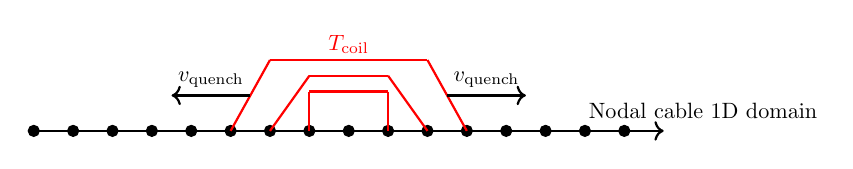
\begin{tikzpicture}[scale = 1]
\draw [thick, ->] (0.0,0.0) -- (8.0,0);
\foreach \t in {0,0.5,1,...,7.5}
\filldraw[black] ({\t},0) circle (2pt);
\node[scale = 0.8] at (8.5,0.25) {Nodal cable 1D domain};
\draw [thick, red] (3.5,0) -- (3.5,0.5);
\draw [thick, red] (3.5,0.5) -- (4.5,0.5);
\draw [thick, red] (4.5,0.5) -- (4.5,0);
\draw [thick, red] (3,0) -- (3.5,0.7);
\draw [thick, red] (3.5,0.7) -- (4.5,0.7);
\draw [thick, red] (4.5,0.7) -- (5,0);
\draw [thick, red] (2.5,0) -- (3,0.9);
\draw [thick, red] (3,0.9) -- (5,0.9);
\draw [thick, red] (5,0.9) -- (5.5,0);
\draw [thick, ->] (5.25,0.45) -- (6.25,0.45);
\node[scale = 0.8] at (5.75,0.65) {$v_\text{quench}$};
\draw [thick, ->] (2.75,0.45) -- (1.75,0.45);
\node[scale = 0.8] at (2.25,0.65) {$v_\text{quench}$};
\node[scale = 0.8, red] at (4,1.1) {$T_\text{coil}$};
\end{tikzpicture}
\caption{Schematic temperature propagation with quench velocity modelling.}
\label{fig:modelling_approach}
\end{figure}

The idea of a quench velocity modelling is based on calculating/imposing quench velocity by an outsourced external routine. Such an approach allows one to have the quench wave implicitly solved. An accurate solution at the quench front is not required and the temperature in this region is approximated, knowing that it is placed between two extreme temperatures (either inside or outside of the quenched zone). As a result, the mesh refinement along the coil length is not needed anymore and the numerical model of smaller size is solved. To sum up, the numerical model still calculates the heat balance equation but with a fixed and relatively coarse mesh along the coil. Solving the quench propagation by means of a quench velocity method assumes that, while  simulating the heat propagation during a quench, the quench front velocity is known and estimated separately beforehand. 

\subsection{Co-simulation Modelling}
\label{subsection:quench_velocity_cosimulation}

This part of the section describes how the quench velocity method is applied in ANSYS simulations. In order to distinguish the quenched zone from the non-quenched one, the superconducting cable is divided into two domains as presented in Fig. \ref{fig:ansys_material_assignment}. The non-quenched part is characterised by nearly zero-resistivity (not zero for the sake of numerical stability) whereas the quenched cable has non-linear resistivity properties of the strand composite as described in (\ref{eqn: p_dens_equiv}). The non-linear resistivity is reassigned at each time step as the quench propagates in ANSYS model.

\begin{figure}[H]
\centering
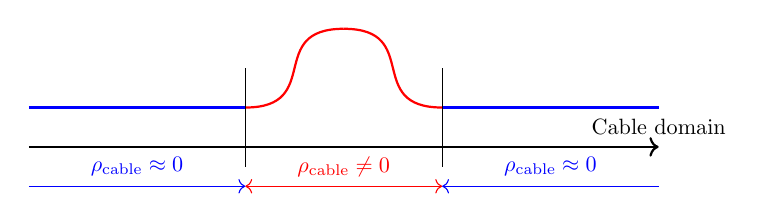
\begin{tikzpicture}[scale = 1]
\draw [thick, ->] (0.0,0.0) -- (8.0,0);
\draw [thick, blue] (0.0,0.5) -- (2.75,0.5);
\draw [thick, blue] (5.25,0.5) -- (8.0,0.5);
\draw [thick, red] (2.75,0.5) .. controls +(0:1cm) and +(180:1cm) .. (4.0,1.5);
\draw [thick, red] (4.0,1.5) .. controls +(0:1cm) and +(180:1cm) .. (5.25,0.5);
\draw [thin] (2.75,-0.25) -- (2.75,1.0);
\draw [thin] (5.25,-0.25) -- (5.25,1.0);
\draw [thin, red, <->] (2.75,-0.5) -- (5.25,-0.5);
\draw [thin, blue, ->] (0.0,-0.5) -- (2.75,-0.5);
\draw [thin, blue, <-] (5.25,-0.5) -- (8.0,-0.5);
\node[scale = 0.8] [color = red] at (4.0,-0.25) {$\rho_\text{cable} \neq 0$};
\node[scale = 0.8] [color = blue] at (1.375,-0.25) {$\rho_\text{cable} \approx 0$};
\node[scale = 0.8] [color = blue] at (6.625,-0.25) {$\rho_\text{cable} \approx 0$};
\node[scale = 0.8] at (8.0,+0.25) {Cable domain};
\end{tikzpicture}
\caption{ANSYS cable domain assignment.}
    \label{fig:ansys_material_assignment}
\end{figure}

The reassignment of material properties should be handled by an external routine which controls the propagation of quench in time. In this case, one should deal with a co-simulation of a numerical solver (in this case ANSYS) and a quench velocity estimator. This problem can be handled by means of a one-directional (Fig. \ref{fig:unidirectional_coupling_scheme}) or a bi-directional (Fig. \ref{fig:bidirectional_coupling_scheme}) exchange of signals. In a one-directional case, the numerical solver is provided with a quench front position from the previous communication point $T_{j-1}$ and calculates temperature distribution in the current communication point $T_j$. When a bi-directional case is considered, the external routine is provided with the data from the numerical solver at point $T_j$ to estimate quench velocity at point $T_{j-1}$ up to the point $T_j$. The line which describes the information direction is marked in red in Fig. \ref{fig:bidirectional_coupling_scheme}. In both cases the initial quench length is assumed at the beginning of the co-simulation. Between the time steps of the external routine, the numerical solver can handle the problem with a time step smaller than the communication points $T_j$.

\begin{figure}[H]
\centering
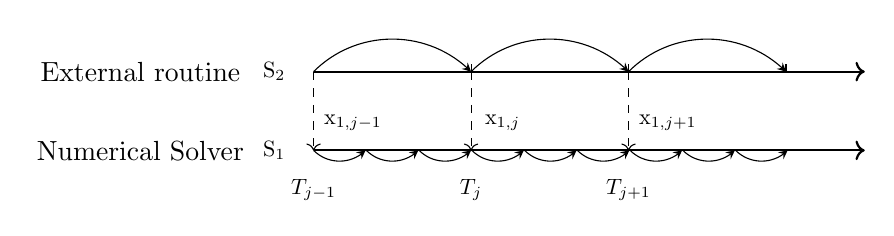
\begin{tikzpicture}[scale = 1]
\draw[thick,->] (0,1) -- (7,1);
\draw (2, 1) -- (2, 1.1);
\draw (4, 1) -- (4, 1.1);
\draw (6, 1) -- (6, 1.1);
\foreach \t in {1,3,5}
\draw [-stealth, bend angle=45, bend left, color = black]  ({\t-1},1) to (\t+1,1);
\draw[thick,->] (0,0) -- (7,0);
\draw (2, 1) -- (2, 1.1);
\draw (4, 1) -- (4, 1.1);
\draw (6, 1) -- (6, 1.1);
\foreach \t in {0.66,1.33,...,6.33}
\draw [-stealth, bend angle=45, bend right]  ({\t-0.66},0) to (\t,0);
\node[scale = 0.8] at (0, -0.5) {$T_{j-1}$};
\node[scale = 0.8] at (2,-0.5) {$T_j$};
\node[scale = 0.8] at (4,-0.5) {$T_{j+1}$};
\draw[dashed, ->] (0,1) -- (0,0);
\draw[dashed, ->] (2,1) -- (2,0);
\draw[dashed, ->] (4,1) -- (4,0);
\node[scale = 0.8] at (-0.5, 0) {$\text{S}_1$};
\node[scale = 0.8] at (-0.5, 1) {$\text{S}_2$};
\node[scale = 0.8] at (0.5, 0.35) {$\text{x}_{1,j-1}$};
\node[scale = 0.8] at (2.4, 0.35) {$\text{x}_{1,j}$};
\node[scale = 0.8] at (4.5, 0.35) {$\text{x}_{1,j+1}$};
\node[color = black] at (-2.2,1.0)	{External routine};
\node at (-2.2,0)	{Numerical Solver};
\end{tikzpicture}
\caption{Schematic representation of one-directional coupling between a numerical solver and quench velocity estimator.}
\label{fig:unidirectional_coupling_scheme}
\end{figure}

\begin{figure}[H]
\centering
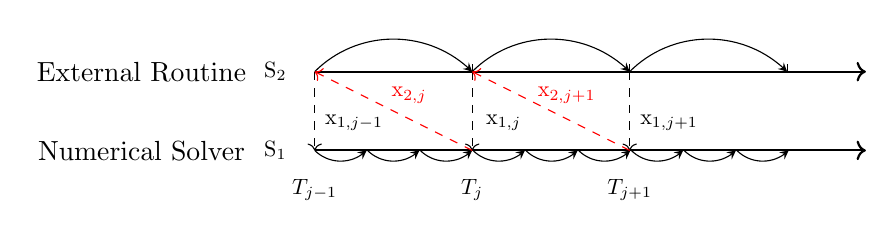
\begin{tikzpicture}[scale = 1]
\draw[thick,->] (0,1) -- (7,1);
\draw (2, 1) -- (2, 1.1);
\draw (4, 1) -- (4, 1.1);
\draw (6, 1) -- (6, 1.1);
\foreach \t in {1,3,5}
\draw [-stealth, bend angle=45, bend left, color = black]  ({\t-1},1) to (\t+1,1);
\draw[thick,->] (0,0) -- (7,0);
\draw (2, 1) -- (2, 1.1);
\draw (4, 1) -- (4, 1.1);
\draw (6, 1) -- (6, 1.1);
\foreach \t in {0.66,1.33,...,6.33}
\draw [-stealth, bend angle=45, bend right]  ({\t-0.66},0) to (\t,0);
\node[scale = 0.8] at (0, -0.5) {$T_{j-1}$};
\node[scale = 0.8] at (2,-0.5) {$T_j$};
\node[scale = 0.8] at (4,-0.5) {$T_{j+1}$};
\draw[dashed, ->] (0,1) -- (0,0);
\draw[dashed, ->] (2,1) -- (2,0);
\draw[dashed, ->] (4,1) -- (4,0);
\draw[dashed, red, ->] (2,0) -- (0,1);
\draw[dashed, red, ->] (4,0) -- (2,1);
\node[scale = 0.8] at (-0.5, 0) {$\text{S}_1$};
\node[scale = 0.8] at (-0.5, 1) {$\text{S}_2$};
\node[scale = 0.8] at (0.5, 0.35) {$\text{x}_{1,j-1}$};
\node[scale = 0.8] at (2.4, 0.35) {$\text{x}_{1,j}$};
\node[scale = 0.8] at (4.5, 0.35) {$\text{x}_{1,j+1}$};
\node[scale = 0.8, red] at (1.2, 0.7) {$\text{x}_{2,j}$};
\node[scale = 0.8, red] at (3.2, 0.7) {$\text{x}_{2,j+1}$};
\node[color = black] at (-2.2,1.0)	{External Routine};
\node at (-2.2,0)	{Numerical Solver};
\end{tikzpicture}
\caption{Schematic representation of bi-directional coupling between a numerical solver and quench velocity estimator.}
\label{fig:bidirectional_coupling_scheme}
\end{figure}

Provided that data exchange between an external routine and a numerical solver occurs at communication times $T_j$, the quench velocity algorithm is solved as described in Algorithm \ref{alg:weak_coupling}.

\begin{algorithm}
  \caption{Weak Coupling between a numerical solver and quench velocity estimator.}
  \label{alg:weak_coupling}
  \begin{algorithmic}[1]
    \STATE assume initial quench position $x_{1,j-1}$ 
    \STATE \textbf{for} $j=1,2,...,N$ \textbf{do}
    \STATE \hspace{0.5cm} solve temperature distribution at time $T_j$
    \STATE \hspace{0.5cm} extrapolate solver results $x_{2,j}$ to external routine time $T_{j-1}$ (only for bi-directional case)
    \STATE \hspace{0.5cm} estimate new quench position $x_{1,j}$ for a quench front
    \STATE \hspace{0.5cm} assign quench position $x_{1,j}$ to new nodes for solver time  $T_j$
  \end{algorithmic}
\end{algorithm}

As already mentioned, the quench velocity can be: $(i)$ based on available measurements, $(ii)$ calculated numerically, $(iii)$ calculated analytically according to quench velocity equations available in literature. The first 2 above-mentioned methods to calculate quench velocity would require one-directional exchange of signals. If quench velocity is estimated analytically, one can choose between the one-directional and bi-directional case depending on whether the formula requires input data from the solver such as an updated material properties repository.

For the purpose of this thesis, the quench velocity is estimated numerically based on a one-directional exchange of signals.


% QUENCH VELOCITY MODELLING BENCHMARKING
\clearpage
\section{Quench Velocity Modelling Benchmarking}
\label{section:quench_velocity_benchmarking}

The aim of this section is to compare the proposed quench velocity - based analysis with a standard heat balance equation modelling in ANSYS. The elements to compare are: 
\begin{itemize}
    \item number of nodes,
    \item time step applied,
    \item relative error, 
    \item computing time.
\end{itemize}

The \nth{1} step is to conduct a heat balance equation - based analysis. It will serve for two purposes: ($i$) reference model for relative error, ($ii$) quench velocity value to be used in quench velocity - based model. The \nth{2} stage aims at conducting quench velocity - based simulations with quench velocity value obtained from 1D numerical heat balance equation - based models. 

In this section, all material properties are based on NIST standards described in Appendix \ref{appendix_material_properties_description}. The analysis is conducted for two cases separately: 
\begin{itemize}
    \item 1D strand analysis without insulation layer,
    \item 1D strand analysis with an external insulation layer.
\end{itemize}



\subsection{Analysis without Insulation}
\label{subsection:quench_velocity_benchmarking_no_insulation}

\subsubsection{Heat Balance - Based Analysis}

In this study, the standard thermal numerical analysis based on LINK33 element was conducted in ANSYS. The geometric assumptions as well as initial conditions were the same as in Section~\ref{section: 1D_quench_propagation_no_insulation}. It is interesting to mention that the initial Gaussian profile of temperature over the domain (see Fig. \ref{fig: init_gauss_temp_distr}) stores a different value of energy in the strand depending on the longitudinal mesh size. The initial energy in the discretised strand domain is calculated as
\begin{equation}
    E_\text{initial} = \sum_{i=1}^{n-1} V_{i,i+1}~C_\text{v, strand}\left(\frac{T_i+T_{i+1}}{2}\right)~\frac{T_i+T_{i+1}}{2},
\end{equation}
where $n$ -- number of nodes in the initially quenched zone, $V_{i,~i+1}$ -- volume of the domain between two neighbouring nodes, $C_\text{v, strand}$ -- volumetric heat capacity calculated for an average temperature, $T_i$ -- temperature of node $i$, $T_{i+1}$ -- temperature of the neighbouring node $i+1$.

The relation between the initially deposited energy in the strand and the number of nodes over a 1 metre-long domain is presented in Fig. \ref{fig: q_vel_modelling_energy_deposition}. The exact energy deposition starts converging for the number of mesh nodes in the range of 1000 nodes. The lower number of nodes would cause the quench front being too slow with respect to the result obtained from a denser mesh.

\begin{figure}[H]
\centering
    \begin{tikzpicture}
        \begin{axis}[
          width=0.7\linewidth, 
          height = 4.5cm,
          xmode=log,
          xlabel={Number of nodes},
          ylabel={Deposited Energy, $\text{J}$},
          xmin=50.0,
          xmax=5000.0
          ]
          \addplot[blue, mark=*] table[x=nodes,y=energy,col sep=comma] {sections/q_vel_modelling_benchmarking/figures/results_no_insulation/energy_deposition.csv};
        \end{axis}
    \end{tikzpicture}
    \caption{Initial energy deposition along the strand as a function of number of nodes in a 1 metre-long domain.}
    \label{fig: q_vel_modelling_energy_deposition}
\end{figure}

As described in Fig.~\ref{fig:block_diagram_benchmarking_methodology_no_insulation} in the previous section, the first analysis was conducted with the longitudinal mesh size of 1~mm and the time step range $t=[100, 1000]~\upmu \text{s}$. There were three iteration loops~$i$ conducted within the time stepping iteration loop, as shown in Table~\ref{table: 1d_qv_benchmarking_results_heat_balance_no_insulation}. The relative error of the time step range $t=[10, 100]~\upmu \text{s}$ remained below 1\% with respect to the time step range $t= [1, 10]~\upmu \text{s}$. Therefore, the condition is satisfied for the analysis with the time step range of $t=[10, 100]~\upmu \text{s}$ and this analysis is sent to the mesh size loop.

\begin{table}[H]
    \caption{Quench results for analysed time step ranges.} 
    \vspace{-1.em} 
    \fontsize{10}{10}
    \selectfont 
    \renewcommand{\arraystretch}{1.5}
    \begin{center}
        \begin{tabular}{ cccc }  
        \hline
        time step range & [1, 10] & [10, 100] & [100, 1000] \\
        $v_\text{quench, average}$ & 6.80 & 6.81 & 7.1 \\
        $E_\text{r}$ & - & 0.17\% & 4.26\% \\
        \hline 
        \end{tabular}
    \end{center}  
     \label{table: 1d_qv_benchmarking_results_heat_balance_no_insulation} 
 \end{table}

In the mesh size loop, the reference analysis from the time step loop was compared with the analysis conducted with a doubled number of nodes over a 1 metre-long strand. As presented in Fig.~\ref{fig: q_vel_modelling_v_quench_rel_error_no_insulation}, the relative error with respect to the average quench velocity value during the analysis is less than 1\%. 

\begin{figure}[H]
\centering
    \begin{tikzpicture}
        \begin{axis}[
          width=0.7\linewidth, 
          height = 4.5cm,
          xlabel={Time, $\text{s}$},
          ylabel={Relative error, \%},
          xtick={0,0.02,0.04,...,0.1},
          xticklabel style={/pgf/number format/fixed},
          xmin=0.0,
          xmax=0.1
          ]
          \addplot[blue, mark=*] table[x=time,y=1000_nodes_rel_error,col sep=comma] {sections/q_vel_modelling_benchmarking/figures/results_no_insulation/v_quench_rel_error.csv};
          \addplot[blue, dashed] table[x=time,y=1000_nodes_av_rel_error,col sep=comma] {sections/q_vel_modelling_benchmarking/figures/results_no_insulation/v_quench_rel_error.csv};
        \end{axis}
    \end{tikzpicture}
    \caption{Incremental and average (dashed) quench velocity relative error for 1000 nodes with respect to 2000 nodes for the time step range of $t=[10, 100]~\upmu \text{s}$.}
    \label{fig: q_vel_modelling_v_quench_rel_error_no_insulation}
\end{figure}

Therefore, the reference analysis for the benchmarking purposes with quench velocity-based simulations is the one with the mesh size of 1~mm and with the time step range of $t=[10, 100]~\upmu \text{s}$. The analysis settings used for the benchmarking with the quench velocity-based method are summarised in Table~\ref{table: 1d_qv_benchmarking_reference_analysis_settings_no_insulation}. 

\begin{table}[H]
    \caption{Input parameters of the reference standard solution.} 
    \vspace{-1.em} 
    \fontsize{10}{10}
    \selectfont 
    \renewcommand{\arraystretch}{1.5}
    \begin{center}
        \begin{tabular}{ ccc }  
        \hline
        parameter & value & unit \\
        \hline
        mesh size & 1 & [mm] \\
        time step range & [10, 100] & [\textmu s] \\
        $v_\text{quench, average}$ & 6.81 & [m/s] \\
        \hline 
        \end{tabular}
    \end{center}  
     \label{table: 1d_qv_benchmarking_reference_analysis_settings_no_insulation} 
 \end{table}

The analysis chosen as a reference for benchmarking purposes is an acceptable compromise between the accuracy and the computing time. As presented in Fig. \ref{fig: q_vel_modelling_heat_balance_computing_time_no_insulation}, in 1D thermal quench propagation, computing time rises monotonically with mesh refinement while keeping the time step range equal to $t=[10, 100]~\upmu \text{s}$\footnote{The analysis was performed on the following calculation unit: Intel(R) Xeon(R) CPU E5-2667 V4 @~3.20 GHz (2~processors) with RAM 128 GB.}.

\begin{figure}[H]
\centering
    \begin{tikzpicture}
        \begin{axis}[
          width=0.7\linewidth, 
          height = 4.5cm,
          xlabel={Number of nodes},
          ylabel={Computing time, $\text{s}$},
          xmin=0,
          xtick={0,1000,2000,...,5000},
          xticklabel style={/pgf/number format/fixed},
          xmax=5000,
          legend pos=north west
          ]
          \addplot[blue, mark=*] table[x=nodes,y=time,col sep=comma] {sections/q_vel_modelling_benchmarking/figures/results_no_insulation/heat_balance_computing_time.csv};
          \addplot[red, dashed] table[x=nodes,y=linear_approx,col sep=comma] {sections/q_vel_modelling_benchmarking/figures/results_no_insulation/heat_balance_computing_time.csv};
          
          \legend{
          computing time,
          linear approximation
          }
          
        \end{axis}
    \end{tikzpicture}
    \caption{Computing time as a function of number of nodes.}
    \label{fig: q_vel_modelling_heat_balance_computing_time_no_insulation}
\end{figure}

\subsubsection{Quench Velocity - Based Analysis}

In this analysis, an electro-thermal simulation using the LINK68 element is conducted in ANSYS. LINK68 is a uniaxial 1D element which can be used in a 3D space. It has the ability to conduct heat and electrical current along its nodes with an internal heat source corresponding to the Joule effect. Similarly to the element LINK33, it is used for steady-state and transient numerical problems. In preceding simulations, the Joule effect was implemented by introducing a power source over the entire strand domain as a function of resistivity (being a function of temperature). The usage of LINK68 allows for omitting this step since the solver computes the heat source by an internal routine based on material property state. The element requires electrical resistivity of the composite strand~\cite{ansys_element_manual}.

In order to obtain the same solver settings as in case of the analysis performed in Section~\ref{section:quench_velocity_benchmarking_no_insulation_heat_balance}, the 1D strand domain was grounded and constant value of current was applied, as shown in Fig. \ref{fig: q_vel_benchmarking_electrical_settings}.

\begin{figure}[H]
\centering
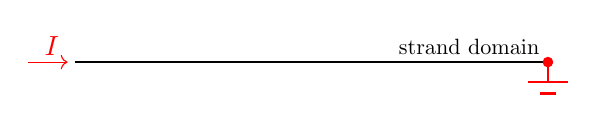
\begin{tikzpicture}[scale = 1]
\draw[thick, black] (-3,0) -- (3,0);
\filldraw[red] (3,0) circle (0.06);
\draw[thick, red] (3,0) -- (3,-0.25);
\draw[thick, red] (2.75,-0.25) -- (3.25,-0.25);
\draw[thick, red] (2.9,-0.4) -- (3.1,-0.4);
\draw[thin, red, ->] (-3.6,0) -- (-3.1,0);
\node[scale=0.8] at (2,0.2) {strand domain};
\node[scale=1.0, red] at (-3.3,0.2) {$I$};
\end{tikzpicture}
\caption{Electric boundary conditions.}
\label{fig: q_vel_benchmarking_electrical_settings}
\end{figure}

The additional parameters related to the co-simulation of a quench velocity-based analysis are shown in Table \ref{table: 1d_qv_benchmarking_geometry_parameters_quench_velocity}. At the communication time instants of the co-simulation, the external routine exchanges data with ANSYS in order to update the material properties in the model. 

\begin{table}[H]
    \caption{Analysis input parameters.} 
    \vspace{-1.em} 
    \fontsize{10}{10}
    \selectfont 
    \renewcommand{\arraystretch}{1.5}
    \begin{center}
        \begin{tabular}{ ccc }  
        \hline
        parameter & value & unit \\
        \hline
        communication time step & 0.0025 & [s] \\
        average quench velocity & 6.81 & [m/s] \\
        \hline 
        \end{tabular}
    \end{center}  
     \label{table: 1d_qv_benchmarking_geometry_parameters_quench_velocity} 
 \end{table}

First of all, the possibility of increasing the time step range was checked. Two time step ranges were chosen: $t=\{[10, 100], [100, 1000]\}~\upmu \text{s}$. The relative error with respect to the average quench velocity cannot be compared in this case because the quench velocity is an input parameter for the quench velocity-based analysis. Therefore, the relative error is estimated for the resistive voltage with respect to the reference standard solution. The relative error for two time step ranges varied by less than 0.01\%. Therefore, in all further simulations with varying mesh size, the time step range is equal to $t=[100, 1000]~\upmu \text{s}$.

The study over a 1 metre-long domain was conducted with a varying number of nodes, $n=\{30, 50, 100, 500, 1000\}$. The geometric assumptions as well as initial conditions were the same as in Section~\ref{section: 1D_quench_propagation_no_insulation} without a heat source. As presented in Fig.~\ref{fig: q_vel_benchmarking_temp_distr_over_strand_no_insulation}, quench velocity-based co-simulation results in the quench front remaining behind the benchmark solution. 

\begin{figure}[H]
\centering
    \begin{tikzpicture}
        \begin{axis}[
          no markers,
          width=0.8\linewidth, 
          height = 5.0cm,
          xlabel={$L_\text{strand},~\text{m}$},
          ylabel={$T,~\text{K}$},
          xmin=0.0,
          ymin=0.0,
          xmax=1.0,
          legend pos=north east
          ]
          
        %   Initial temperature curve for the mesh used in quench velocity modelling 
          \addplot[black] table[x=position,y=t_0,col sep=comma] {sections/q_vel_modelling_benchmarking/figures/results_no_insulation/quench_velocity_50_nodes_no_insulation.csv};
          
        %   Heat Balance Equation plots
          \addplot[red] table[x=position,y=t_0_03,col sep=comma] {sections/q_vel_modelling_benchmarking/figures/results_no_insulation/heat_balance_1000_nodes_benchmark.csv};
          \addplot[red] table[x=position,y=t_0_06,col sep=comma] {sections/q_vel_modelling_benchmarking/figures/results_no_insulation/heat_balance_1000_nodes_benchmark.csv};
          \addplot[red] table[x=position,y=t_0_1,col sep=comma] {sections/q_vel_modelling_benchmarking/figures/results_no_insulation/heat_balance_1000_nodes_benchmark.csv};

        %   Quench Velocity Modelling plots
          \addplot[blue] table[x=position,y=t_0_03,col sep=comma] {sections/q_vel_modelling_benchmarking/figures/results_no_insulation/quench_velocity_50_nodes_no_insulation.csv};
          \addplot[blue] table[x=position,y=t_0_06,col sep=comma] {sections/q_vel_modelling_benchmarking/figures/results_no_insulation/quench_velocity_50_nodes_no_insulation.csv};
          \addplot[blue] table[x=position,y=t_0_1,col sep=comma] {sections/q_vel_modelling_benchmarking/figures/results_no_insulation/quench_velocity_50_nodes_no_insulation.csv};
          
          \legend{
          $T_\text{init}$ profile,
          heat balance,,,
          quench velocity
          }
        \end{axis}
        
        \draw[black, thick, ->] (2,3) -- (3,3);
        \node[scale = 1] at (3.8, 3) {$\vec{v}_\text{quench}$}; 
        
    \end{tikzpicture}
    \caption{Temperature distribution of a heat balance-based benchmark solution and a quench velocity-based solution with 50 nodes along the domain for three time steps: $t=\{0.03, 0.06, 0.1\}$~s with a specified direction of quench velocity, $\vec{v}_\text{quench}$.}
    \label{fig: q_vel_benchmarking_temp_distr_over_strand_no_insulation}
\end{figure}

The reasons for differences in the results are twofold:
\begin{enumerate}
    \item In Fig.~\ref{fig:unidirectional_coupling_scheme} presented in Section~\ref{section:quench_velocity_cosimulation}, it was explained that the external routine updates resistive material properties at communication point $T_{j-1}$ and ANSYS solves the case for $T_{j}$. Therefore, the quenched zone is underestimated and 'delayed' with respect to the standard quench numerical solution. To reduce this error, the number of communication points was increased to~40 which corresponds to a time window of $t=2.5~\text{ms}$. 
    \item In quench velocity modelling, the material properties assignment to the strand is binary. The material has resistive properties of the strand composite above its critical temperature and no resistance below this value. The transition region of current sharing temperature is not taken into account. Therefore, the strand might not warm up sufficiently at the transition region.
\end{enumerate}

As shown in Fig. \ref{fig: q_vel_modelling_res_volt_benchmarking}, the resistive voltage in quench velocity-based method follows the curve of the benchmark solution. However, the resistive voltage remains underestimated with respect to the standard solution.

\begin{figure}[H]
\centering
    \begin{tikzpicture}
        \begin{axis}[
          width=0.7\linewidth, 
          height = 4.5cm,
          xlabel={Time, $\text{s}$},
          ylabel={Resistive Voltage, $\text{V}$},
          xticklabel style={/pgf/number format/fixed},
          yticklabel style={/pgf/number format/fixed},
          xmin=0.0,
          xmax=0.1,
          legend pos=north west
          ]
          \addplot[blue, mark=*] table[x=time,y=50_nodes_quench_velocity,col sep=comma] {sections/q_vel_modelling_benchmarking/figures/results_no_insulation/quench_velocity_res_volt_benchmarking.csv};
          \addplot[red] table[x=time,y=heat_balance_benchmark,col sep=comma] {sections/q_vel_modelling_benchmarking/figures/results_no_insulation/quench_velocity_res_volt_benchmarking.csv};
          
          \legend{
          quench velocity,
          heat balance
          }
          
        \end{axis}
    \end{tikzpicture}
    \caption{Resistive voltage comparison for standard numerical solution and quench velocity-based simulation with 50 nodes along the domain.}
    \label{fig: q_vel_modelling_res_volt_benchmarking}
\end{figure}

As presented in Fig.~\ref{fig: q_vel_modelling_res_volt_rel_error}, one can state that the longer the simulation lasts, the lower relative error is obtained with respect to the reference solution. The relative error converges because the quenched zone propagates with time. For 50 nodes, the relative error converges below -5\%.
In Fig. \ref{fig: q_vel_modelling_res_volt_rel_error}, the case with 1000 nodes also shows the similar shape of the relative error curve. For that reason, the error cannot be explained by the decrease of mesh density, as it was presented in Fig.~\ref{fig: q_vel_modelling_energy_deposition} where the initial energy deposition may result in slowing down the quench propagation. In this case, the benchmark standard numerical solution was of the same mesh size. Therefore, the error in the given range has to be accepted if one conducts a quench velocity-based analysis.

\begin{figure}[H]
\centering
    \begin{tikzpicture}
        \begin{axis}[
          width=0.7\linewidth, 
          height = 4.5cm,
          xlabel={Time, $\text{s}$},
          ylabel={Relative error, \%},
          xticklabel style={/pgf/number format/fixed},
          xmin=0.0,
          xmax=0.1,
          legend pos=south east
          ]
          \addplot[blue, mark=*] table[x=time,y=50_nodes,col sep=comma] {sections/q_vel_modelling_benchmarking/figures/results_no_insulation/quench_velocity_res_volt_rel_error.csv};
          \addplot[red, mark=*] table[x=time,y=100_nodes,col sep=comma] {sections/q_vel_modelling_benchmarking/figures/results_no_insulation/quench_velocity_res_volt_rel_error.csv};
          \addplot[green, mark=*] table[x=time,y=1000_nodes,col sep=comma] {sections/q_vel_modelling_benchmarking/figures/results_no_insulation/quench_velocity_res_volt_rel_error.csv};
          \addlegendimage{/pgfplots/refstyle=plot_resistive_voltage}\addlegendentry{50 nodes}
          \addlegendimage{/pgfplots/refstyle=plot_resistive_voltage}\addlegendentry{100 nodes}
          \addlegendimage{/pgfplots/refstyle=plot_resistive_voltage}\addlegendentry{1000 nodes}
          
        \end{axis}
    \end{tikzpicture}
    \caption{Relative error of resistive voltage for 50, 100 and 1000 nodes used for quench velocity-based simulation.}
    \label{fig: q_vel_modelling_res_volt_rel_error}
\end{figure}

As shown in Fig. \ref{fig: q_vel_modelling_hot_spot_rel_error}, the relative error in case of the hot spot temperature did not exceed -2\% during the entire analysis and also converged to the -0.5\% independently of the applied mesh size as the simulation proceeded. 

\begin{figure}[H]
\centering
    \begin{tikzpicture}
        \begin{axis}[
          width=0.7\linewidth, 
          height = 4.5cm,
          xlabel={Time, $\text{s}$},
          ylabel={Relative error, \%},
          xticklabel style={/pgf/number format/fixed},
          xmin=0.0,
          xmax=0.1,
          legend pos=south east
          ]
          \addplot[blue, mark=*] table[x=time,y=50_nodes,col sep=comma] {sections/q_vel_modelling_benchmarking/figures/results_no_insulation/quench_velocity_hot_spot_rel_error.csv};
          \addplot[red, mark=*] table[x=time,y=100_nodes,col sep=comma] {sections/q_vel_modelling_benchmarking/figures/results_no_insulation/quench_velocity_hot_spot_rel_error.csv};
          \addplot[green, mark=*] table[x=time,y=1000_nodes,col sep=comma] {sections/q_vel_modelling_benchmarking/figures/results_no_insulation/quench_velocity_hot_spot_rel_error.csv};
          \addlegendimage{/pgfplots/refstyle=plot_resistive_voltage}\addlegendentry{50 nodes}
          \addlegendimage{/pgfplots/refstyle=plot_resistive_voltage}\addlegendentry{100 nodes}
          \addlegendimage{/pgfplots/refstyle=plot_resistive_voltage}\addlegendentry{1000 nodes}
          
        \end{axis}
    \end{tikzpicture}
    \caption{Relative error of hot spot for 50, 100 and 1000 nodes used for quench velocity-based simulation.}
    \label{fig: q_vel_modelling_hot_spot_rel_error}
\end{figure}



\subsection{Analysis with Insulation}
\label{subsection:quench_velocity_benchmarking_with_insulation}
\input{sections/q_vel_modelling_benchmarking/quench_velocity_benchmarking_with_insulation.tex}

% ALGORITHMS AND PYTHON IMPLEMENTATION
\clearpage
\section{Algorithms}
\label{section:algorithms}

In a thermal problem, there are two phenomena to be analysed important for the quench simulations: $(i)$~longitudinal propagation of quench, $(ii)$~transverse heat flow inside the insulation layer. The quench velocity-based methodology can only be used in the \nth{1} case. The heat flow across the insulation is an important factor if a multi-strand model is analysed. In order to conduct a multi-strand thermal analysis using quench velocity-based approach, the following simulation tools and algorithms ought to be developed.

\begin{enumerate}
\item Electro-thermal model simulating longitudinal quench propagation.
\item Thermal model simulating transverse thermal propagation across insulation.
\item Algorithm mapping multi-strand and multi-dimensional magnet geometry onto 1D coil.
\item Algorithm calculating quench position in time which is based on a quench velocity function.
\item Algorithm which would assign the nodes to the quenched and non-quenched zones in a discretised domain in time.
\item Algorithm detecting new quenches in a multi-strand domain if the quenched winding heats up the neighbouring ones across the insulation.
\end{enumerate}

This chapter describes all the aforementioned algorithms except for the quench velocity algorithm which was described in Section~\ref{subsection:quench_velocity_cosimulation}.

\subsection{Multidimensional Mapping Algorithm}
\label{subsection:multidimensional_mapping_algorithm}

The multidimensional mapping algorithm aims at translating a multidimensional geometry into an imaginary 1D strand. This procedure serves for $(i)$ assigning the~magnetic field to the~windings separately, $(ii)$ mapping the~geometry for the~quench detection algorithm. 

As illustrated in Fig.~\ref{fig: 3d_coil_illustation_with_2d_b_field}, a multi-strand domain is subjected to a time- and space-dependent magnetic field. Thus, every winding is exposed to a different magnetic field which also varies with a current change. From the magnetic analysis standpoint, it is assumed that the coil is infinitely long, allowing for using a 2D magnetic map from the centre of a~magnet cross-section.

\begin{figure}[H]
    \centering
    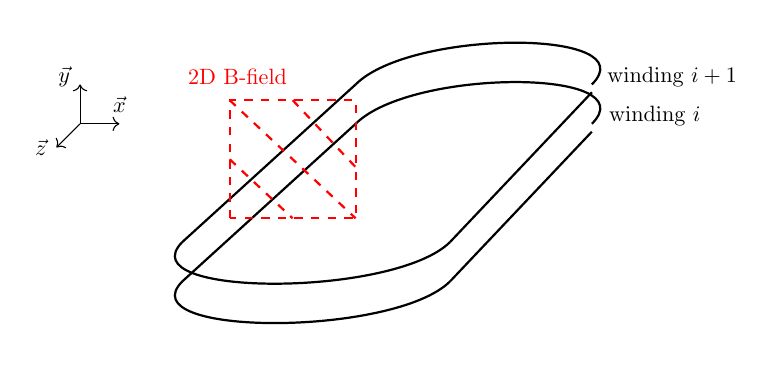
\begin{tikzpicture}[scale = 1]
        
        \foreach \y in {0,0.5} 
        \draw[thick,  black] (0.2,\y) -- (2,\y+1.9);
        \foreach \y in {0,0.5} 
        \draw[thick, black] (.2,\y) .. controls +(45:-1cm) and +(45:-1cm) .. (-3.2,\y);
        \foreach \y in {0,0.5} 
        \draw[thick,  black] (-3.2,\y) -- (-1,\y+2.0);
        \foreach \y in {0,0.5} 
        \draw[thick, black] (-1,\y+2) .. controls +(45:1cm) and +(45:1cm) .. (2,\y+2);
        
        \draw[thick, dashed, red] (-2.6,0.8) rectangle (-1.0,2.3);
        \draw[thick, dashed, red] (-2.6,1.55) -- (-1.8, 0.8);
        \draw[thick, dashed, red] (-2.6,2.3) -- (-1.0, 0.8);
        \draw[thick, dashed, red] (-1.8,2.3) -- (-1.0, 1.45);
        
        \node[scale = 0.8] at (2.8,2.1) {winding $i$};
        \node[scale = 0.8] at (3.02,2.6) {winding $i+1$};
        \node[red, scale = 0.8] at (-2.5,2.6) {2D B-field};
        
        \draw[black, ->] (-4.5,2) -- (-4.8,1.7);
        \draw[black, ->] (-4.5,2) -- (-4.5,2.5);
        \draw[black, ->] (-4.5,2) -- (-4,2);
        
        \node[scale = 0.8] at (-4,2.25) {$\vec{x}$};
        \node[scale = 0.8] at (-4.7,2.6) {$\vec{y}$};
        \node[scale = 0.8] at (-5,1.7) {$\vec{z}$};
        
    \end{tikzpicture}
    \caption{Schematic of an assignment of a magnetic field to a multi-strand domain.}
    \label{fig: 3d_coil_illustation_with_2d_b_field}
\end{figure}

The magnetic field is assigned to every winding separately, as shown in Fig.~\ref{fig:ansys_python_mapping scheme}. Each of them is characterised by a different thermal and electrical material property. The multi-strand geometry is translated into a realistic one-dimensional cable with a length $L_\text{coil}$ equal to the total coil length. Each part of the coil corresponding to one winding, is subject to a~different magnetic field~$B_\text{n}$. Similarly to Fig.~\ref{fig: 1d_strand_geometry}, the one-dimensional coordinate system $\bar x$ in Fig.~\ref{fig:ansys_python_mapping scheme} represents the~longitudinal direction of the coil. 

\begin{figure}[H]
\centering
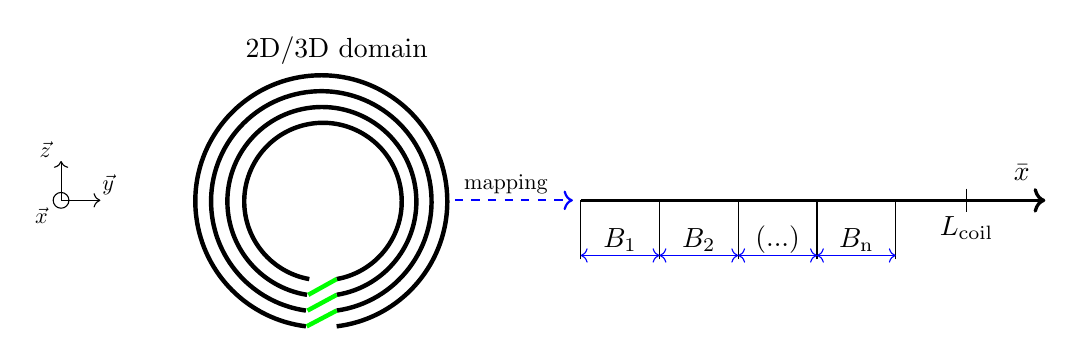
\begin{tikzpicture}[scale = 1]
\draw [ultra thick] (0,0) arc (-80:260:1);
\draw [ultra thick] (0,-0.2) arc (-81:261:1.2);
\draw [ultra thick] (0,-0.4) arc (-82:262:1.4);
\draw [ultra thick] (0,-0.6) arc (-83:263:1.6);
\draw [ultra thick, green] (0,0) -- (-0.36,-0.2);
\draw [ultra thick, green] (0,-0.2) -- (-0.37,-0.4);
\draw [ultra thick, green] (0,-0.4) -- (-0.38,-0.6);
\node[scale = 1.0] at (0,2.9) {2D/3D domain};
\draw [thick, dashed, blue, ->] (1.5,1) -- (3,1);
\node[scale = 0.8] at (2.15,1.2) {mapping};
\draw [very thick, ->] (3.1,1) -- (9,1);
\foreach \t in {3.1, 4.1, ..., 7.1}
\draw [thin] ({\t},0.25) -- ({\t},1);
\foreach \t in {3.1, 4.1, ..., 6.1}
\draw [thin, blue, <->] ({\t},0.3) -- ({\t+1},0.3);

\draw [thin] (8.0,1.15) -- (8.0,0.85);

\node[scale = 1.0] at (3.6,0.5) {$B_1$};
\node[scale = 1.0] at (4.6,0.5) {$B_2$};
\node[scale = 1.0] at (5.6,0.5) {(...)};
\node[scale = 1.0] at (6.6,0.5) {$B_\text{n}$};
\node[scale = 1.0] at (8,0.65) {$L_\text{coil}$};

\node[scale = 1.0] at (8.7,1.35) {$\bar x$};

\draw (-3.5,1) circle (0.1cm);
\draw[black, ->] (-3.5,1) -- (-3.5,1.5);
\draw[black, ->] (-3.5,1) -- (-3,1);

\node[scale = 0.8] at (-3.75,0.8) {$\vec{x}$};
\node[scale = 0.8] at (-2.9,1.2) {$\vec{y}$};
\node[scale = 0.8] at (-3.7,1.65) {$\vec{z}$};

\end{tikzpicture}
\caption{Mapping scheme of a magnetic field onto an imaginary 1D coil.}
\label{fig:ansys_python_mapping scheme}
\end{figure}



\subsection{Node Searching Algorithm}
\label{subsection:node_searching_algorithm}

Regardless the manner how the quench velocity is calculated, the external routine will always understand the quench length as if it was a continuous function of time. Therefore, it is expected that the calculated quench position~$L$ in a given time will differ from the available positions of a discrete meshed geometry in a numerical solver. Therefore, it is important to create an algorithm assigning the nodes to the quenched and non-quenched zones in a discretised domain.

The quench zone assignment algorithm is presented in Fig. \ref{fig:node_search_algo}. It searches the node $N_\text{search}$ whose geometric position is below the assumed error,~$\epsilon$ compared to the quench length $L$ calculated on the side of an external routine estimating quench velocity. At each time step the algorithm checks whether $N_\text{search}$ is within the space $N$ and ${N+x}$ when jump search is considered. In case of a dense mesh, the step control doubles if the right zone ${[N+(a-1)x, N+ax]}$ is not found after 5 iterations. When the node space ${[N+(a-1)x, N+ax]}$ contains the searched node, it uses the binary search to find the node fulfilling the condition ${\mid L(N_\text{search}) - L \mid \geq \epsilon}$. 

\begin{figure}[H]
\centering
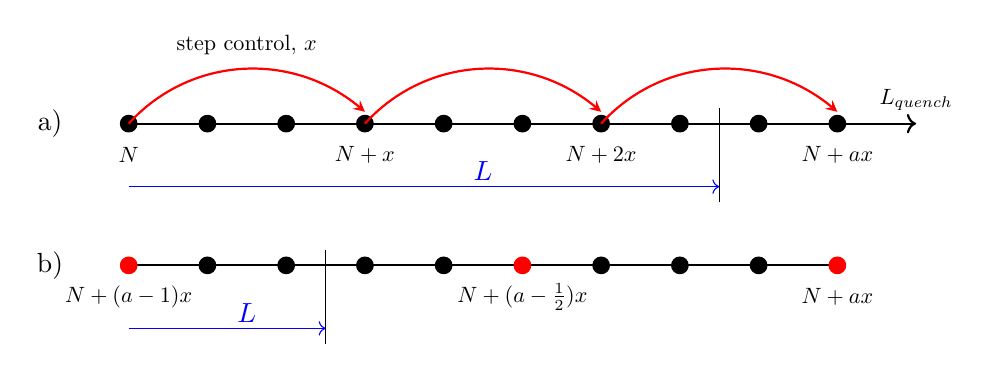
\begin{tikzpicture}[scale = 1]
\draw[thick,->] (0,1) -- (10,1);
\foreach \t in {0,1,...,9}
\filldraw[black] ({\t},1) circle (3pt);
\foreach \t in {1,4,7}
\draw [thick, -stealth, bend angle=45, bend left, color = red]  ({\t-1},1) to (\t+2,1.15);
\node[scale = 0.8] at (1.5, 2) {step control, $x$};
\node[scale = 0.8] at (0, 0.6) {$N$};
\node[scale = 0.8] at (3, 0.6) {$N+x$};
\node[scale = 0.8] at (6, 0.6) {$N+2x$};
\node[scale = 0.8] at (9, 0.6) {$N+ax$};
\node[scale = 0.8] at (10, 1.3) {$L_{quench}$};
\draw[thin, blue, ->] (0,0.2) -- (7.5,0.2);
\draw[thin, black] (7.5,0) -- (7.5,1.2);
\node[scale = 1, blue] at (4.5, 0.4) {$L$};
\node at (-1, 1) {a)};

\draw[thick] (0,-0.8) -- (9,-0.8);
\foreach \t in {1,2,3,4,6,7,8}
\filldraw[black] ({\t},-0.8) circle (3pt);
\foreach \t in {0,5,9}
\filldraw[red] ({\t},-0.8) circle (3pt);
\node[scale = 0.8] at (0, -1.2) {$N+(a-1)x$};
\node[scale = 0.8] at (5, -1.2) {$N+(a-\frac{1}{2})x$};
\node[scale = 0.8] at (9, -1.2) {$N+ax$};
\draw[thin, black] (2.5,-1.8) -- (2.5,-0.6);
\draw[thin, blue, ->] (0,-1.6) -- (2.5,-1.6);
\node[scale = 1, blue] at (1.5, -1.4) {$L$};
\node at (-1, -0.8) {b)};
\end{tikzpicture}
\caption{ a) Jump search; b) Bi-section search.}
\label{fig:node_search_algo}
\end{figure}

Provided that searching starts at node $N$, quench length calculated in the external routine is $L$, searching error is $\epsilon$, step control equals $x$, number of step controls applied equals $a$, the problem is solved as described in Algorithm \ref{alg:node_searching}.

\begin{algorithm}[H]
    \caption{Quench Zone Assignment Algorithm.}
    \label{alg:node_searching}
    \begin{algorithmic}[1]
    \STATE \textbf{while} $L(N) < L$ \textbf{do}
    \STATE \hspace{0.5cm} increase N by step control x
    \STATE \hspace{0.5cm} \textbf{if} number of iterations over x is multiplication of 5 \textbf{do}
    \STATE \hspace{1.0cm} double step control $x$
    \STATE \textbf{while} $\mid L(\frac{2N+(2a-1)x}{2}) - L \mid \geq \epsilon$ \textbf{do}
    \STATE \hspace{0.5cm} \textbf{if} $L(\frac{2N+(2a-1)x}{2}) > L$ \textbf{do}
    \STATE \hspace{1.0cm} continue search in domain $D \in (N+(a-1)x ; \frac{2N+(2a-1)x}{2})$
    \STATE \hspace{0.5cm} \textbf{elseif} $L(\frac{2N+(2a-1)x}{2}) < L$ \textbf{do}
    \STATE \hspace{1.0cm} continue search in domain $D \in (\frac{2N+(2a-1)x}{2} ; N+ax)$
    \end{algorithmic}
\end{algorithm}

The algorithm also works if the mesh is too coarse or if $\epsilon$ is too small to find the right node with binary search. In such a case, the closest node to the length obtained analytically is chosen.

\subsection{Quench Detection Algorithm}
\label{subsection:quench_detection_algorithm}

In this section, an algorithm detecting new quenches in a multi-strand domain is presented. It is only valid when a multi-filament geometry is analysed when a quenched winding heats up the neighbouring ones across the insulation layer. In detail, the algorithm detects quenches and initiates a new quench front propagation  when the temperature outside of the quenched zone exceeds the critical temperature of a superconductor. It is responsible for turn-to-turn propagation across the insulation layer between windings.

Provided that searching starts at node $N$, winding number is $W$, magnetic field strength of the winding $W$ is $B_W$, node temperature is $T_N$ and critical temperature of related winding is $T_{c,W}$, the problem is solved as described in Algorithm \ref{alg:quench_detection}.

\begin{algorithm}
    \caption{Quench detection algorithm description}
    \label{alg:quench_detection}
    \begin{algorithmic}[1]
    \STATE \textbf{for} $N$ which is not quenched \textbf{do}
    \STATE \hspace{0.5cm} check the winding $W$ which node $N$ belongs to
    \STATE \hspace{0.5cm} assign magnetic field $B_W$ of given winding $W$
    \STATE \hspace{0.5cm} calculate $T_{c,W}$ for given magnetic field $B_W$
    \STATE \hspace{0.5cm} \textbf{if} $T(N) > T_{c,W}$
    \STATE \hspace{1.0cm} assign node $N$ to list of newly quenched nodes
    \end{algorithmic}
\end{algorithm}

% PYTHON IMPLEMENTATION
\clearpage
\section{Analysis Implementation in Python}
\label{section:python_implementation}

This part describes the implementation of quench velocity modelling in ANSYS by means of external Python scripts. Python architecture is designed to perform the following tasks: 

\begin{itemize}
\item launch ANSYS simulation,
\item create APDL scripting commands in order to communicate with ANSYS,
\item create 3D ANSYS meshed geometry of a magnet with given geometrical specifications,
\item map meshed 3D ANSYS geometry to create 1D imaginary coil in Python with specified position of each node,
\item assign material properties to ANSYS geometry with respect to an external magnetic field map,
\item calculate quench velocity at each time step, 
\item assign quenched zone to newly quenched nodes,
\item detect quench at new windings due to turn-to-turn propagation in the 3D ANSYS geometry.
\end{itemize}
 
The simulation is carried out in ANSYS in "-aas" mode (batch mode) while Python main execution script controls it. Except for the above-mentioned tasks, Python script is also in charge of the majority of post-processing. ANSYS sends the results as well as the data about mesh by means of text files which are uploaded to Python as $numpy$ arrays afterwards. The exemplary ANSYS compilation with Python is presented in Appendix \ref{appendix:python_ansys_compilation}. The Python script architecture is depicted in Fig. \ref{fig:python_script_architecture}.

\begin{figure}[H]
\centering
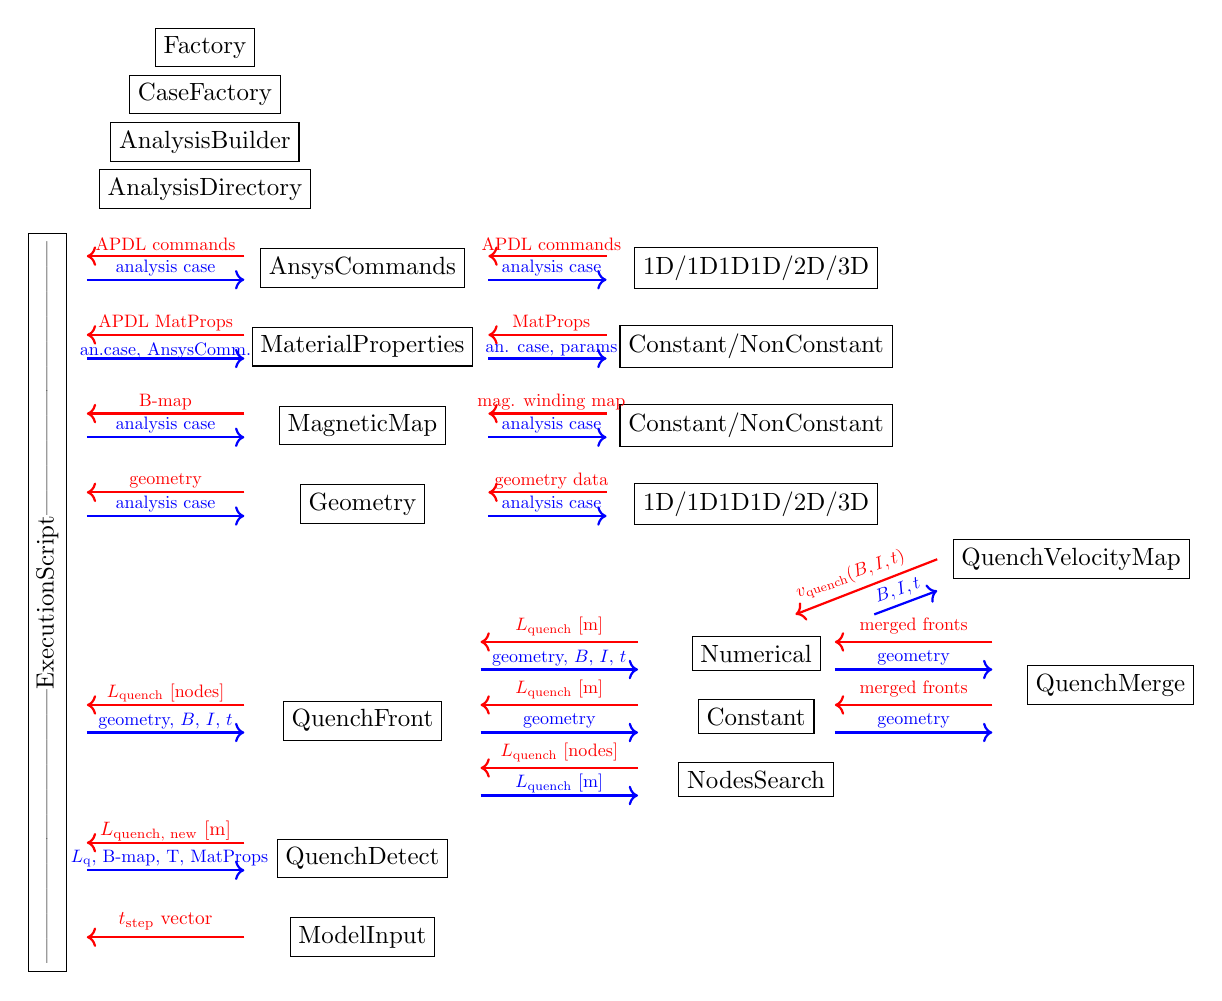
\begin{tikzpicture}[scale = 1]
\node[scale = 0.9, rotate=90] at (1,-4.25) [draw] {|||||||||||ExecutionScript|||||||||||};

\node[scale = 0.9] at (3,2.8) [draw] {Factory};
\node[scale = 0.9] at (3,2.2) [draw] {CaseFactory};
\node[scale = 0.9] at (3,1.6) [draw] {AnalysisBuilder};
\node[scale = 0.9] at (3,1) [draw] {AnalysisDirectory};

\node[scale = 0.9] at (5,0) [draw] {AnsysCommands};
\node[scale = 0.9] at (10,0) [draw] {1D/1D1D1D/2D/3D};
\draw [thick, red, ->] (3.5,0.15) -- (1.5,0.15);
\node[scale = 0.65, red] at (2.5,0.3) {APDL commands};
\draw [thick, blue, ->] (1.5,-0.15) -- (3.5,-0.15);
\node[scale = 0.65, blue] at (2.5,0) {analysis case};
\draw [thick, red, ->] (8.1,0.15) -- (6.6,0.15);
\node[scale = 0.65, red] at (7.4,0.3) {APDL commands};
\draw [thick, blue, ->] (6.6,-0.15) -- (8.1,-0.15);
\node[scale = 0.65, blue] at (7.4,0) {analysis case};

\node[scale = 0.9] at (5,-1) [draw] {MaterialProperties};
\node[scale = 0.9] at (10,-1) [draw] {Constant/NonConstant};
\draw [thick, red, ->] (3.5,-0.85) -- (1.5,-0.85);
\node[scale = 0.65, red] at (2.5,-0.7) {APDL MatProps};
\draw [thick, blue, ->] (1.5,-1.15) -- (3.5,-1.15);
\node[scale = 0.65, blue] at (2.5,-1.05) {an.case, AnsysComm.};
\draw [thick, red, ->] (8.1,-0.85) -- (6.6,-0.85);
\node[scale = 0.65, red] at (7.4,-0.7) {MatProps};
\draw [thick, blue, ->] (6.6,-1.15) -- (8.1,-1.15);
\node[scale = 0.65, blue] at (7.4,-1.05) {an. case, params};

\node[scale = 0.9] at (5,-2) [draw] {MagneticMap};
\node[scale = 0.9] at (10,-2) [draw] {Constant/NonConstant};
\draw [thick, red, ->] (3.5,-1.85) -- (1.5,-1.85);
\node[scale = 0.65, red] at (2.5,-1.7) {B-map};
\draw [thick, blue, ->] (1.5,-2.15) -- (3.5,-2.15);
\node[scale = 0.65, blue] at (2.5,-2) {analysis case};
\draw [thick, red, ->] (8.1,-1.85) -- (6.6,-1.85);
\node[scale = 0.65, red] at (7.4,-1.7) {mag. winding map};
\draw [thick, blue, ->] (6.6,-2.15) -- (8.1,-2.15);
\node[scale = 0.65, blue] at (7.4,-2) {analysis case};

\node[scale = 0.9] at (5,-3) [draw] {Geometry};
\node[scale = 0.9] at (10,-3) [draw] {1D/1D1D1D/2D/3D};
\draw [thick, red, ->] (3.5,-2.85) -- (1.5,-2.85);
\node[scale = 0.65, red] at (2.5,-2.7) {geometry};
\draw [thick, blue, ->] (1.5,-3.15) -- (3.5,-3.15);
\node[scale = 0.65, blue] at (2.5,-3) {analysis case};
\draw [thick, red, ->] (8.1,-2.85) -- (6.6,-2.85);
\node[scale = 0.65, red] at (7.4,-2.7) {geometry data};
\draw [thick, blue, ->] (6.6,-3.15) -- (8.1,-3.15);
\node[scale = 0.65, blue] at (7.4,-3) {analysis case};

\node[scale = 0.9] at (5,-5.75) [draw] {QuenchFront};
\draw [thick, red, ->] (3.5,-5.55) -- (1.5,-5.55);
\node[scale = 0.65, red] at (2.5,-5.4) {$L_\text{quench}~\text{[nodes]}$};
\draw [thick, blue, ->] (1.5,-5.9) -- (3.5,-5.9);
\node[scale = 0.65, blue] at (2.5,-5.75) {geometry, $B$, $I$, $t$};

\node[scale = 0.9] at (10,-4.9) [draw] {Numerical};
\draw [thick, red, ->] (8.5,-4.75) -- (6.5,-4.75);
\draw [thick, blue, ->] (6.5,-5.1) -- (8.5,-5.1);
\node[scale = 0.65, red] at (7.5,-4.55) {$L_\text{quench}~\text{[m]}$};
\node[scale = 0.65, blue] at (7.5,-4.95) {geometry, $B$, $I$, $t$};

\node[scale = 0.9] at (10,-5.7) [draw] {Constant};
\draw [thick, red, ->] (8.5,-5.55) -- (6.5,-5.55);
\draw [thick, blue, ->] (6.5,-5.9) -- (8.5,-5.9);
\node[scale = 0.65, red] at (7.5,-5.35) {$L_\text{quench}~\text{[m]}$};
\node[scale = 0.65, blue] at (7.5,-5.75) {geometry};

\node[scale = 0.9] at (10,-6.5) [draw] {NodesSearch};
\draw [thick, red, ->] (8.5,-6.35) -- (6.5,-6.35);
\draw [thick, blue, ->] (6.5,-6.7) -- (8.5,-6.7);
\node[scale = 0.65, red] at (7.5,-6.15) {$L_\text{quench}~\text{[nodes]}$};
\node[scale = 0.65, blue] at (7.5,-6.55) {$L_\text{quench}~\text{[m]}$};

\node[scale = 0.9] at (14.5,-5.3) [draw] {QuenchMerge};
\draw [thick, red, ->] (13,-4.75) -- (11,-4.75);
\draw [thick, blue, ->] (11,-5.1) -- (13,-5.1);
\node[scale = 0.65, red] at (12,-4.55) {merged fronts};
\node[scale = 0.65, blue] at (12,-4.95) {geometry};

\draw [thick, red, ->] (13,-5.55) -- (11,-5.55);
\draw [thick, blue, ->] (11,-5.9) -- (13,-5.9);
\node[scale = 0.65, red] at (12,-5.35) {merged fronts};
\node[scale = 0.65, blue] at (12,-5.75) {geometry};

\node[scale = 0.9] at (14,-3.7) [draw] {QuenchVelocityMap};
\draw [thick, red, ->] (12.3,-3.7) -- (10.5,-4.4);
\draw [thick, blue, ->] (11.5,-4.4) -- (12.3,-4.1);
\node[scale = 0.65, red, rotate=19] at (11.2,-3.9) {$v_\text{quench} (B,I,t)$};
\node[scale = 0.65, blue, rotate=19] at (11.8,-4.1) {$B,I,t$};

\node[scale = 0.9] at (5,-7.5) [draw] {QuenchDetect};
\draw [thick, red, ->] (3.5,-7.3) -- (1.5,-7.3);
\draw [thick, blue, ->] (1.5,-7.65) -- (3.5,-7.65);

\node[scale = 0.7, red] at (2.5,-7.15) {$L_\text{quench, new}$ [m]};
\node[scale = 0.65, blue] at (2.55,-7.5) {$L_\text{q}$, B-map, T, MatProps};

\node[scale = 0.9] at (5,-8.5) [draw] {ModelInput};
\draw [thick, red, ->] (3.5,-8.5) -- (1.5,-8.5);
\node[scale = 0.7, red] at (2.5,-8.3) {$t_\text{step}$ vector};
\end{tikzpicture}
\caption{Python script architecture}
\label{fig:python_script_architecture}
\end{figure}

Fig. \ref{fig:python_script_architecture} describes the Python code consisting of 4 different Classes and one executive script. The \textit{executive\_script} launches the simulation and executes pre-processing, solution as well as post-processing part of ANSYS simulation. It uses the Class \textit{ansys} to translate Python functions into APDL scripting language. The Class \textit{geometry} imports a meshed geometry and assigns the position in space for each node. Then, the class \textit{quench\_velocity} assigns new quench front position at each time step depending on a current quench velocity. Since the Class \textit{quench\_velocity} operates in meters, it requires a separate class \textit{node\_search} which maps a node number for the calculated quench length as described in Section \ref{subsection:node_searching_algorithm}.\\

At this stage, the class \textit{quench\_velocity} assumes that the quench velocity is constant. In further steps, the quench velocity will be estimated in two-way coupling manner as described in Section \ref{subsection:quench_velocity_algorithm}. In order to reach this step, a new Class called \textit{quench\_detection} will be created. It will initialize the new quench front as soon as the critical temperature is achieved outside of the quenched zone of the coil (turn to turn heat propagation).

% SKEW QUADRUPOLE ANALYSIS - QUENCH DETECTION
\clearpage
\section{Skew Quadrupole Quench Detection Analysis}
\label{section:skew_quadrupole_quench_detection_analysis}

This chapter describes the thermal quench analysis of a skew quadrupole developed by LASA laboratories of INFN-Milano. The skew quadrupole belongs to the group of high-order corrector magnets designed for the upgrade of High-Luminosity LHC. Their design assumes using no quench protection devices such as quench heaters or CLIQ except for crowbars \footnote{Describe what crowbars are...}. Therefore, when any of these magnet quenches, the discharge of energy stored in their magnetic field occurs merely by their own rise in resistivity. i.e. they are self-protected.

Quench velocity approach presented in chapter \ref{section:quench_velocity_modelling} is used to analyze the magnet as a 3-dimensional thermal domain. It is verified by comparing the available measurements of a quenched skew quadrupole with the simulation results conducted in ANSYS. One has to remember that the skew quadrupole is the only high-order corrector which has quench protection system installed, i.e. it is not self-protected. However, it has been used for illustration purposes because of its available quench measurements when quench heaters were not used. 

\subsection{Geometry}

Most of the data about the skew quadrupole was presented in Section~\ref{section: 1d_quench_propagation_geometry}. Unlike in 1D analyses presented in previous chapters, when a 3D thermal simulation of a magnet is considered, it is important to specify its winding scheme because the windings interact with each other thermally across the insulation layer. Fig.~\ref{fig:skew_quad_transversal_cross_section} shows the transversal cross-section of one coil of the skew quadrupole. The windings are enclosed within an area of 24.5x27.3~mm. Moreover, each coil is covered with a 1 mm-thick ground insulation layer apart from the insulation between each winding described in Section~\ref{section: 1d_quench_propagation_geometry}. The ground insulation on the internal side of the coil is thinner and equal to 0.15~mm.

\begin{figure}[H]
    \centering
    \begin{tikzpicture}
    \pgftext{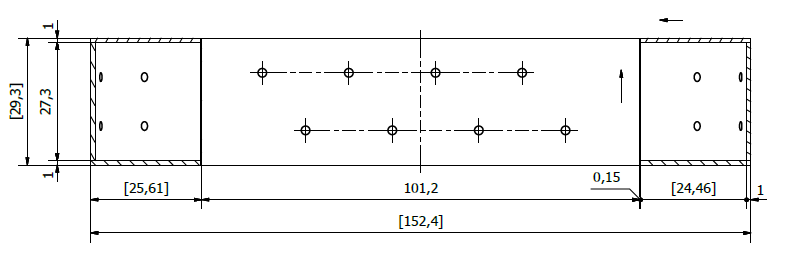
\includegraphics[width=\linewidth]{sections/skew_quad_q_det/figures/skew_quad_design/skew_quad_transversal_cross_section.png}} at (0,0);
    \node[red] at (6.0,2.1) {layers};
    \node[red, rotate=90] at (4.3,0) {turns};
    \draw[red, very thick, dashed] (0.47,-0.95) -- (0.47,2.4); 
    \node[red, scale=0.8] at (1.9,2.1) {coil symmetry};
    \draw[black, very thick, ->] (-4.3,2.1) -- (-4.8,1.8); 
    \node[black, scale=0.8] at (-3.0,2.1) {ground insulation};
    \end{tikzpicture}
    \caption{The transversal cross-section of one coil of a skew quadrupole~\cite{marco_prioli_mails}.}
    \label{fig:skew_quad_transversal_cross_section}
\end{figure}

As shown in Fig.~\ref{fig:winding_arrangement_cross_section}, each coil has 29 turns in each of its 26 layers. In total, the number of windings per coil is 754~\cite{marco_prioli_mails, hl_lhc_tech_design_report_v01}.

\begin{figure}[H]
\centering
    \begin{tikzpicture}
        \begin{axis}[
          width=0.5\linewidth, 
          height=0.5\linewidth,
          xtick={0.0, 24.46},
          ytick={0.0, 27.30},
          xlabel={$x,~\text{mm}~\text{(layers direction)}$},
          ylabel={$y,~\text{mm}~\text{(turns direction)}$},
          xmajorgrids=true,
          ymajorgrids=true,
          xmin=-5.0,
          xmax=29.47,
          ymin=-5.0,
          ymax=32.29,
          ]
          \addplot[blue, only marks, mark size=1pt] table[x=x,y=y,col sep=comma] {sections/skew_quad_q_det/figures/skew_quad_design/winding_location_cross_section.csv};
        \end{axis}
        \draw[scale=0.172, red, very thick, dashed] (2.5,2) -- (2.5,33.0); 
        \node[red, scale=0.8] at (1.9,5.6) {coil symmetry};
        
    \end{tikzpicture}
    \caption{Location of the windings in the cross-section of a half-coil.}
    \label{fig:winding_arrangement_cross_section}
\end{figure}

The winding scheme is shown in Fig.~\ref{fig:winding_scheme_cross_section}. The winding~1 is placed at the bottom left of the 2D cross-section. The last winding number 754 is placed further in the \textit{x}-direction. The \nth{2} half of the coil is a~mirror reflection of the presented winding scheme.

\begin{figure}[H]
\centering
    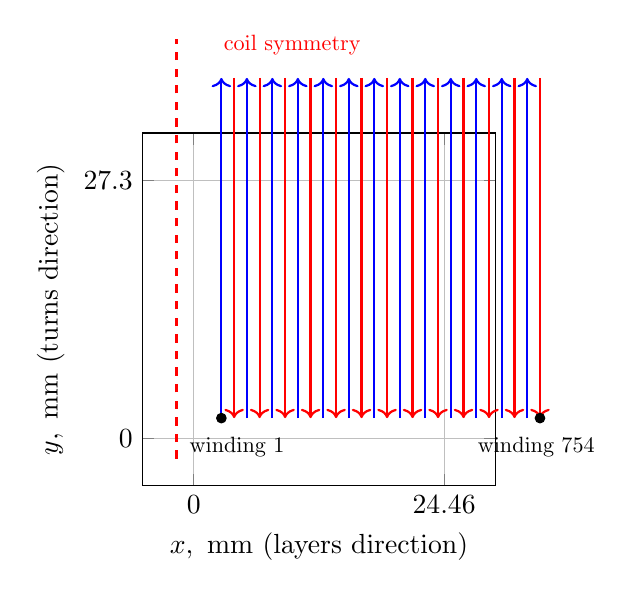
\begin{tikzpicture}
        \begin{axis}[
          width=0.5\linewidth, 
          height=0.5\linewidth,
          xtick={0.0, 24.46},
          ytick={0.0, 27.30},
          xlabel={$x,~\text{mm}~\text{(layers direction)}$},
          ylabel={$y,~\text{mm}~\text{(turns direction)}$},
          xmajorgrids=true,
          ymajorgrids=true,
          xmin=-5.0,
          xmax=29.47,
          ymin=-5.0,
          ymax=32.29,
          ]
        \end{axis}
        \foreach \t in {0.471, 2.353,...,24}
            \draw[scale=0.172, blue, thick, ->] (\t+5.35,5.0) -- (\t+5.35,26.819+3.3); 
        \foreach \t in {1.412, 3.294,...,25}
            \draw[scale=0.172, red, thick, ->] (\t+5.35,26.819+3.3) -- (\t+5.35,5.0);
        \draw[scale=0.172, red, very thick, dashed] (2.5,2) -- (2.5,33.0); 
        \node[red, scale=0.8] at (1.9,5.6) {coil symmetry};
        \filldraw[scale=0.172, black] (0.471+5.35,5.0) circle (10pt);
        \node[black, scale=0.8] at (1.2,0.5) {winding 1};
        \filldraw[scale=0.172, black] (23.996+5.35,5.0) circle (10pt);
        \node[black, scale=0.8] at (5.0,0.5) {winding 754};
        
    \end{tikzpicture}
    \caption{Winding scheme of a single coil of the skew quadrupole.}
    \label{fig:winding_scheme_cross_section}
\end{figure}

The general parameters of the skew quadrupole are summarised in Table~\ref{table:skew_quad_params_table}. In the given magnet, there is only one aperture in which a particle beam travels through. Four coils of the magnet are connected in series and powered by a single power converter. It is interesting to mention that the coil length of only one coil is more than 800~m which is a very large number for thermal quench simulations, as mentioned in Section~\ref{section: 1D_quench_propagation_conclusions}. The operating current of the skew quadrupole is $I=182~\text{A}$.

\begin{table}[H]
    \caption{Geometrical parameters for skew quadrupole \cite{marco_prioli_mails, hl_lhc_tech_design_report_v01}} 
    \vspace{-1.em} 
    \fontsize{10}{10}
    \selectfont 
    \renewcommand{\arraystretch}{1.5}
    \begin{center}
    \begin{tabular}{ ccc }  
    \hline
    parameter & value & unit \\
    \hline
    number of apertures & 1 & [-] \\
    number of circuits & 1 & [-] \\
    aperture size & 150 & [mm]\\
    coil length & 841 & [m] \\
    operating current & 182 & [A] \\
    \hline 
    \end{tabular}
    \end{center}  
     \label{table:skew_quad_params_table} 
 \end{table}

\subsection{Assumptions for Geometry and Material Properties}

Each cable is a single Nb-Ti strand of 0.7 mm diameter with a copper stabilizer. As presented in Fig. \ref{fig:materials_cross_section}, the winding is covered with 0.007 mm thick S2-glass insulation (in red). Then, the winding is immersed in epoxy resin D10 (in blue). The superconducting cable is marked in yellow. Moreover, ground insulation is added on the external side of the coil \cite{hl_lhc_tech_design_report_v01}.

In the superconducting magnet design community, an assumption is often proposed to simulate the materials behaviour outside of the superconducting cable as a single domain characterized by the properties of G10 which is another material widely used in cryogenics. Such an assumption is made in this thesis. The characteristics of all material properties taken into consideration in the analysis are described in Appendix \ref{appendix_material_properties_description}.

\begin{figure}[H]
\centering

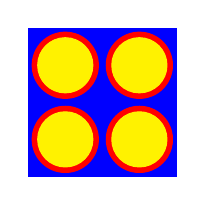
\begin{tikzpicture}[scale = 1]
\filldraw[blue] (-0.941/2,-0.941/2) rectangle (0.941/2,0.941/2);
\filldraw[red] (0,0) circle (0.7/2+0.07);
\filldraw[yellow] (0,0) circle (0.7/2);

\filldraw[blue] (-0.941/2,-0.941/2+0.941) rectangle (0.941/2,0.941/2+0.941);
\filldraw[red] (0,0+0.941) circle (0.7/2+0.07);
\filldraw[yellow] (0,0+0.941) circle (0.7/2);

\filldraw[blue] (-0.941/2+0.941,-0.941/2) rectangle (0.941/2+0.941,0.941/2);
\filldraw[red] (0+0.941,0) circle (0.7/2+0.07);
\filldraw[yellow] (0+0.941,0) circle (0.7/2);

\filldraw[blue] (-0.941/2+0.941,-0.941/2+0.941) rectangle (0.941/2+0.941,0.941/2+0.941);
\filldraw[red] (0+0.941,0+0.941) circle (0.7/2+0.07);
\filldraw[yellow] (0+0.941,0+0.941) circle (0.7/2);

\end{tikzpicture}
    \caption{Cross-section of four neighbouring windings}
    \label{fig:materials_cross_section}
\end{figure}

The stabilizer to superconductor ratio is specified in \cite{hl_lhc_tech_design_report_v01} and is calculated as follows:

\begin{equation}
    \left\{ \begin{array}{ll}
    \frac{f_\text{Cu}}{f_\text{Nb-Ti}} = \frac{A_\text{Cu}}{A_\text{Nb-Ti}} = 2.2\\ \\
    f_\text{Cu} + f_\text{Nb-Ti} = 1
    \end{array} \right.
\end{equation}

At temperatures above quench current flows through both superconductor and copper in parallel connection. What is actually quite surprising, resistivity of a superconductor above critical temperature is much higher that the one of copper. Therefore, it can be assumed that current flows through a stabilizer and only this part contributes to Joule heating. The same occurs with heat conductivity which is much lower for Nb-Ti at higher temperatures. In order to take these characteristics into account during numerical analysis, the winding area is reduced to area of copper. It leads to a formula of reduced diameter presented below.
\begin{equation}
    d_\text{strand, red} = \sqrt{\frac{A_\text{Cu}}{A_\text{strand}}}*d_\text{strand}
\end{equation}

% Since the winding diameter in analysis is smaller than in reality, its equivalent heat capacity must take this correction into account which is shown in the equation below. The representative winding equivalent heat capacity is shown in Fig. \ref{fig:eq_wind_cp}.
% \begin{equation}
%     C_\text{p, equiv} = f_\text{Cu}*C_\text{p, Cu} + f_\text{NbTi}*C_\text{p, NbTi}
% \end{equation}
 
% \begin{figure}[h!]
%     \centering
%     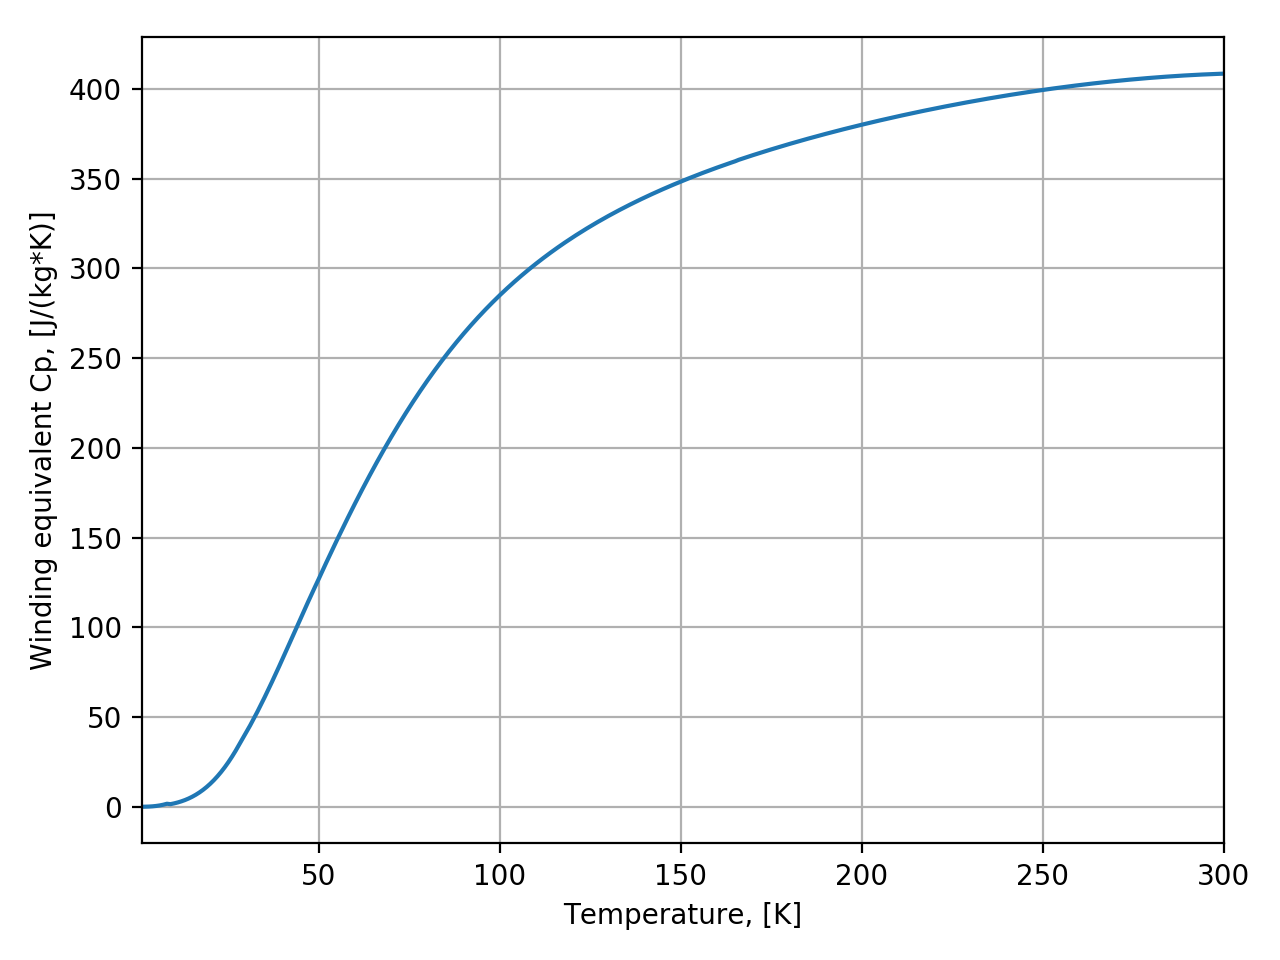
\includegraphics[width=0.35\linewidth]{figures/material_properties/Eq_Cp_plot.png}
%     \caption{Equivalent winding specific heat capacity temperature dependence for \textit{B}=3 T}
%     \label{fig:eq_wind_cp}
% \end{figure}

The geometrical data input are collected and specified altogether in Table \ref{table:skew_quad_params_table}.

\begin{table}[h!]
    \caption{Geometrical parameters for skew quadrupole \cite{hl_lhc_tech_design_report_v01, marco_prioli_mails}} 
    \vspace{-1.em} 
    \fontsize{10}{10}
    \selectfont 
    \renewcommand{\arraystretch}{1.5}
    \begin{center}
    \begin{tabular}{ ccc }  
    \hline
    Aperture & 150 & [mm]\\
    Coil length & 841 & [m] \\
    Number of apertures & 1 & \\
    Number of circuits & 1 & \\
    Strand diameter & 0.7 & [mm] \\
    $\text{A}_\text{Cu}/\text{A}_\text{Nb-Ti}$ \cite{marco_prioli_mails} & 2.2 & \\
    \hline 
    \end{tabular}
    \end{center}  
     \label{table:skew_quad_params_table} 
 \end{table}

Insulation dimensions:

\begin{equation}
    A_\text{ins} = a^2 - \frac{\pi d_\text{strand}^2}{4}
\end{equation}

\begin{equation}
    p_\text{avg} = \frac{4 a + \pi d_\text{strand}}{2} 
\end{equation}

\begin{equation}
    L_\text{ins} = \frac{A_\text{ins}}{p_\text{avg}}
\end{equation}

\begin{equation}
    A_\text{ins,cond} = \frac{\frac{1}{4} A_\text{ins} \cdot L_{winding}}{L_\text{ins}}
\end{equation}

\begin{figure}[H]
\centering
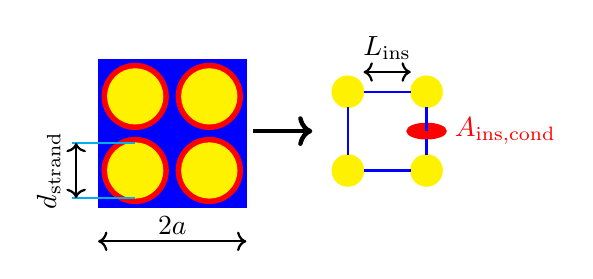
\begin{tikzpicture}[scale = 1]
\filldraw[blue] (-0.941/2,-0.941/2) rectangle (0.941/2,0.941/2);
\filldraw[red] (0,0) circle (0.7/2+0.07);
\filldraw[yellow] (0,0) circle (0.7/2);
\filldraw[blue] (-0.941/2,-0.941/2+0.941) rectangle (0.941/2,0.941/2+0.941);
\filldraw[red] (0,0+0.941) circle (0.7/2+0.07);
\filldraw[yellow] (0,0+0.941) circle (0.7/2);
\filldraw[blue] (-0.941/2+0.941,-0.941/2) rectangle (0.941/2+0.941,0.941/2);
\filldraw[red] (0+0.941,0) circle (0.7/2+0.07);
\filldraw[yellow] (0+0.941,0) circle (0.7/2);
\filldraw[blue] (-0.941/2+0.941,-0.941/2+0.941) rectangle (0.941/2+0.941,0.941/2+0.941);
\filldraw[red] (0+0.941,0+0.941) circle (0.7/2+0.07);
\filldraw[yellow] (0+0.941,0+0.941) circle (0.7/2);
\draw[thick, cyan] (-0.8,0.7/2) -- (0,0.7/2);
\draw[thick, cyan] (-0.8,-0.7/2) -- (0,-0.7/2);
\draw[black, thick, <->] (-0.75,0.7/2) -- (-0.75,-0.7/2);
\node[scale = 1, rotate=90] at (-1.1, 0) {$d_\text{strand}$};
\draw[thick,<->] (-0.941/2,-0.9) -- (0.941*1.5,-0.9);
\node[scale = 1] at (0.941*0.5, -0.7) {$2a$};
\draw[ultra thick,->, black] (1.5,0.5) -- (2.25,0.5);
\filldraw[yellow] (2.7,0) circle (0.2);
\filldraw[yellow] (3.7,0) circle (0.2);
\filldraw[yellow] (3.7,1) circle (0.2);
\filldraw[yellow] (2.7,1) circle (0.2);
\draw[thick, blue] (2.9,0) -- (3.5,0);
\draw[thick, blue] (2.9,1) -- (3.5,1);
\draw[thick, blue] (2.7,0.8) -- (2.7,0.2);
\filldraw[red] (3.7,0.5) ellipse (0.25cm and 0.1cm);
\draw[thick, blue] (3.7,0.8) -- (3.7,0.5);
\draw[thick, blue] (3.7,0.4) -- (3.7,0.2);
\draw[thick, black, <->] (2.9,1.25) -- (3.5,1.25);
\node[scale = 1] at (3.2, 1.55) {$L_\text{ins}$};
\node[scale = 1, red] at (4.7, 0.5) {$A_\text{ins,cond}$};
\end{tikzpicture}
\caption{Cross-sectional of 2D and 1D element}
\end{figure}


\subsection{Quench Measurements}

The quench measurements have been conducted for $I=86~\text{A}$ which is a lower value than the nominal operating current of the skew quadrupole ($I=182~\text{A}$). During the test, the quench has been initiated by discharging a capacitor in series with a 2x2 $\text{mm}^2$ heater attached to the external grounding insulation of the magnet. The voltage drop across the capacitor is presented in Fig. \ref{fig:resistor_voltage_discharge_curve}. By considering the discharge curve as the \nth{1} order, one can deduce the time constant and the resistance of the heater. The obtained data are presented in Table \ref{table:heater_characteristics}.

\begin{figure}[ht!]
    \centering
    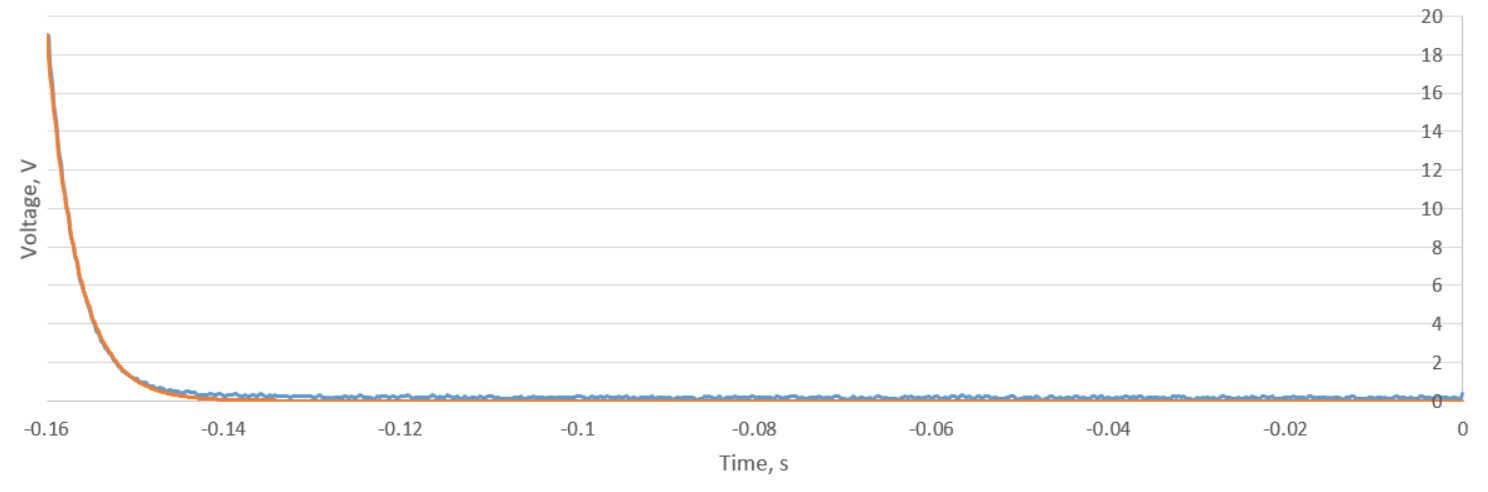
\includegraphics[width=0.65\linewidth]{figures/skew_quad_bcs/voltage_discharge_curve.png}
    \caption{Voltage discharge across the capacitor (in blue) with it \nth{1} order discharge fit (in orange)}
    \label{fig:resistor_voltage_discharge_curve}
\end{figure}

\begin{table}[h!]
    \caption{Heater characteristics} 
    \vspace{-1.em} 
    \fontsize{10}{10}
    \selectfont 
    \renewcommand{\arraystretch}{1.5}
    \begin{center}
    \begin{tabular}{ ccc }  
    \hline
    capacitance & 14 & [mF] \\
    time constant & 3.5 & [ms] \\
    heater resistance & 0.25 & [$\Omega$] \\
    \hline 
    \end{tabular}
    \end{center}  
     \label{table:heater_characteristics} 
 \end{table}

Assuming an adiabatic hot spot (no helium effect), one can deduce total energy input to the magnet as well as power input as a function of time. Power function can be easily deduced from the equation below. The power curve is presented in Fig. \ref{fig:hot_spot_power_input_curve}. After $t=10~\text{ms}$, the value of power is negligible, i.e. the capacitor is fully discharged.
\begin{equation}
    P(t) = \frac{1}{\text{dt}} (\frac{1}{2} \text{C}V^2)
\end{equation}

\begin{figure}[ht!]
    \centering
    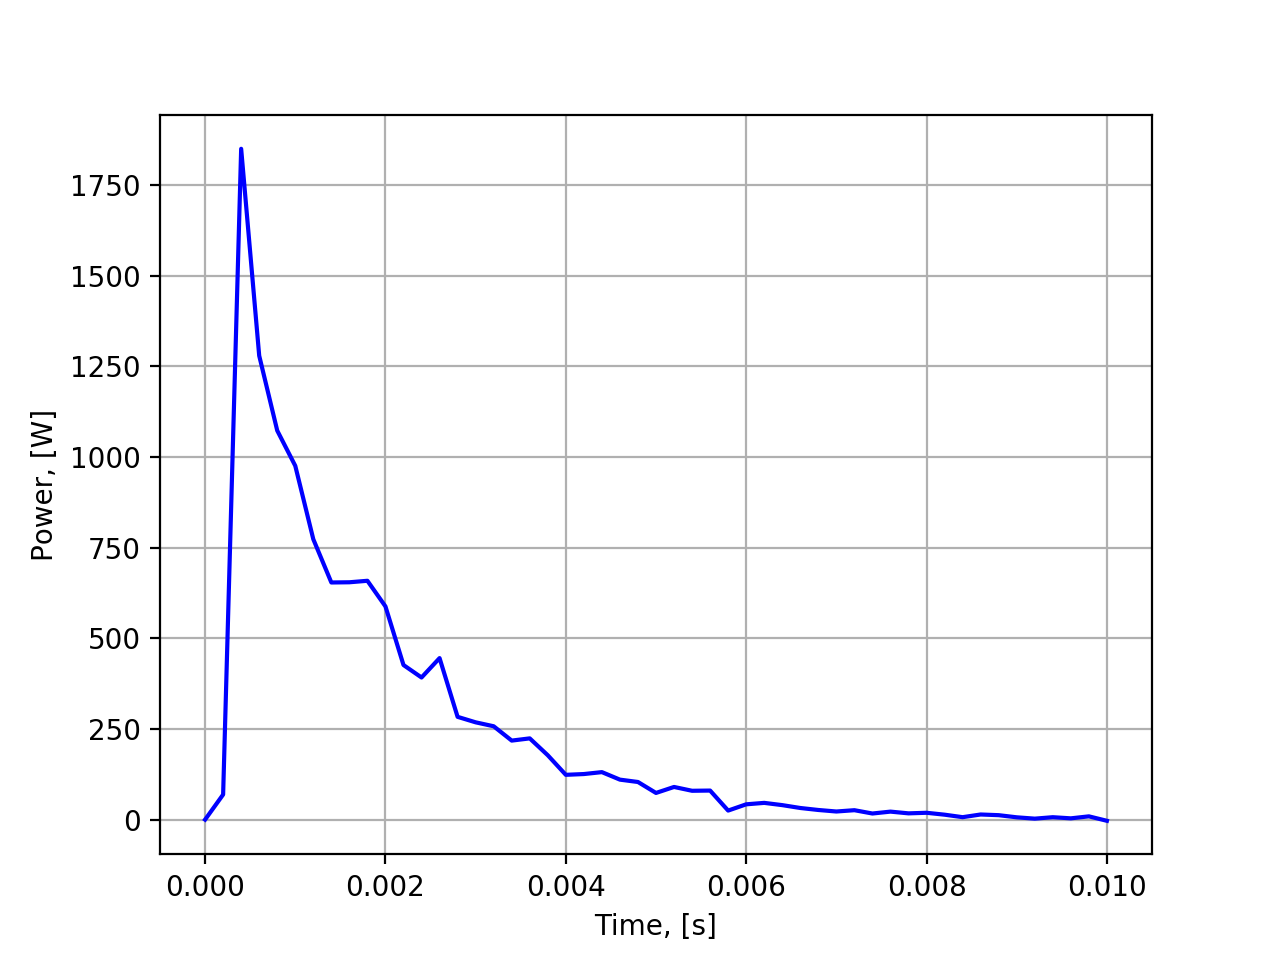
\includegraphics[width=0.45\linewidth]{figures/skew_quad_bcs/Polynomial_Power_Fit.png}
    \caption{Hot spot power input curve}
    \label{fig:hot_spot_power_input_curve}
\end{figure}

When the hot spot is applied, the individual windings start being normal conductive and, therefore resistive. The resistive voltage across the magnet increases, as presented in Fig. \ref{fig:res_volt_curve_quench_detection}. In skew quadrupole, the quench is detected if the magnet resistive voltage equal to at least $V=0.2~\text{V}$ last more than $t=20~\text{ms}$. At $t=0$, the power supply is cut off and the current starts decreasing.

\begin{figure}[ht!]
    \centering
    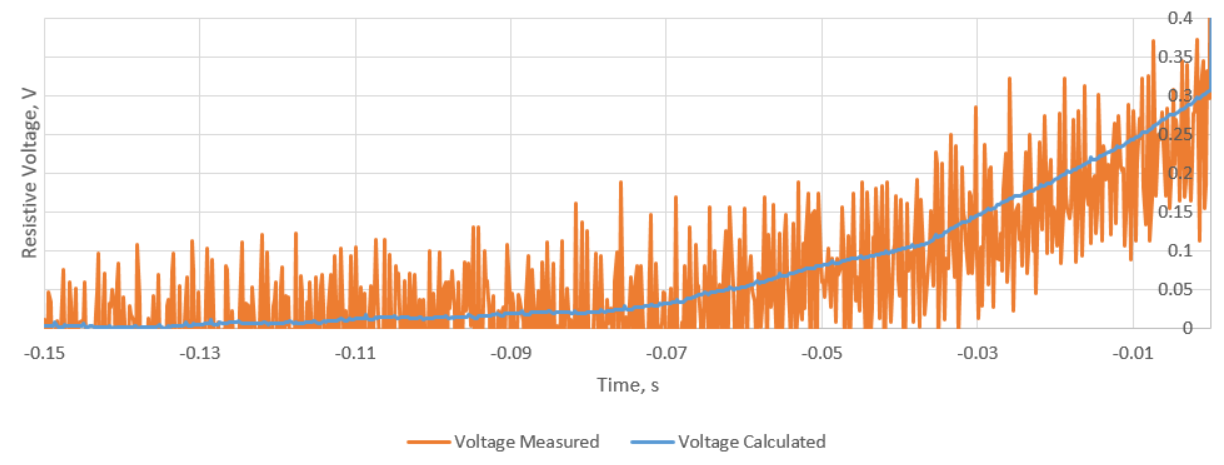
\includegraphics[width=0.6\linewidth]{figures/skew_quad_bcs/quench_det_v_curve.png}
    \caption{Resistive voltage rise until quench detection}
    \label{fig:res_volt_curve_quench_detection}
\end{figure}

\subsection{Magnetic Field Mapping}
Until the quench is detected, the current inside the magnet is constant and equal to $I=86~\text{A}$. Therefore, the magnetic field inside the magnet does not vary in time. The analysis of steady-state magnetic field in the middle of the magnet for this value of current was conducted at INFN-Milano in OPERA software \cite{samuele_mariotto_mails}. A 2D interpolation had to be conducted in order to fit the OPERA mesh with the windings' position. For each winding, it is assumed that it is subjected to the magnetic field from the centre of its cross-section estimated by the interpolation map presented in Fig. \ref{fig:Quad_Mag_contour1}.

\begin{figure}[ht!]
    \centering
    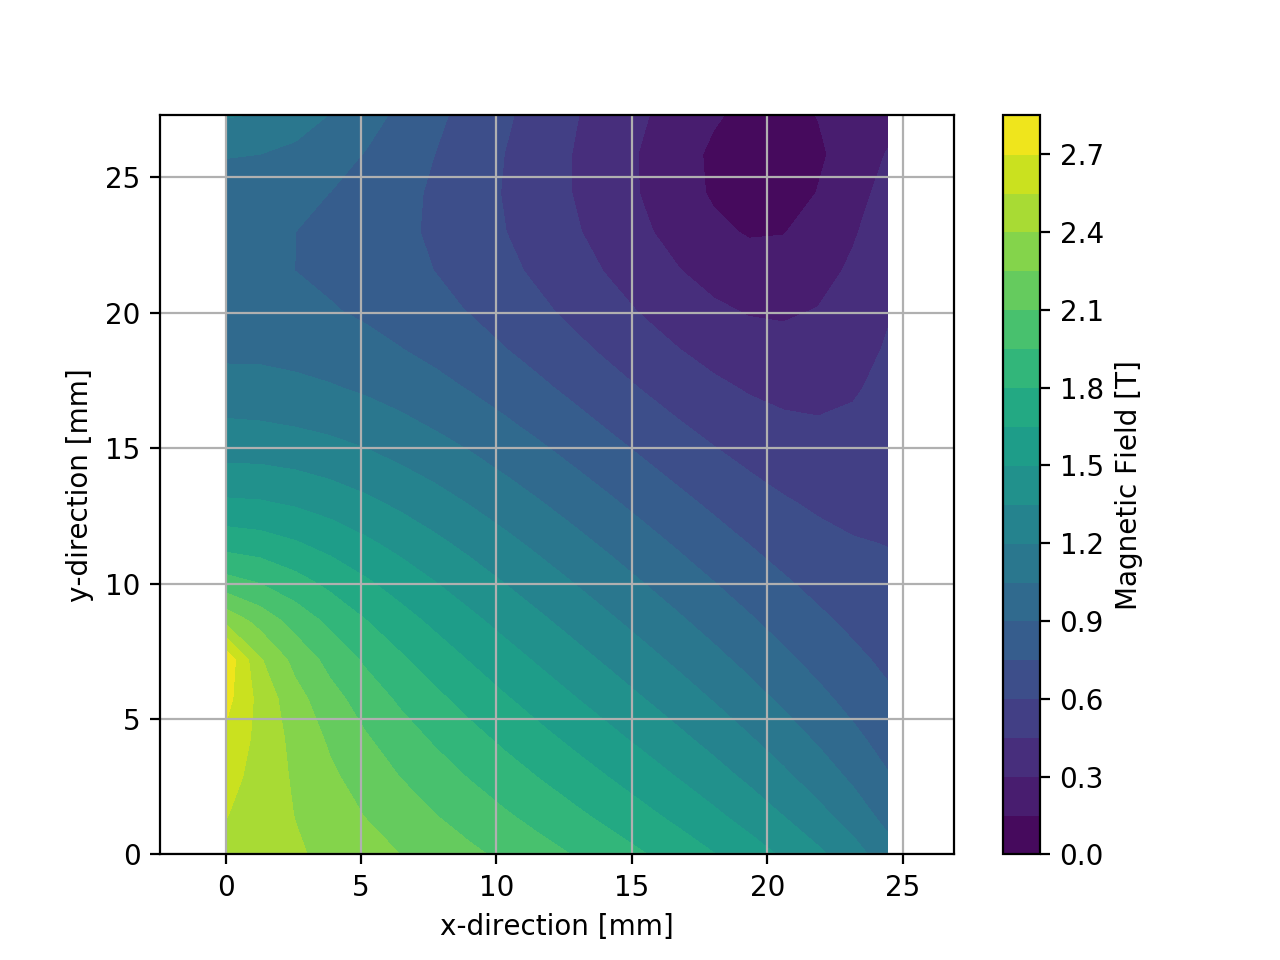
\includegraphics[width=0.49\linewidth]{figures/skew_quad_bcs/magnetic_field_mapping/Quadrupole_Magnetic_Colour_plot.png}
    \caption{Resultant magnetic field strength in the cross-section of skew quadrupole}
    \label{fig:Quad_Mag_contour1}
\end{figure}

\subsection{Initial Conditions...}

Thermal diffusivity is calculated as follows: 
\begin{equation}
    \alpha_{strand} = \frac{k_{Cu}}{\rho_{Cu} \cdot C_{p, equiv}}
\end{equation}

\begin{figure}
\centering
\begin{tikzpicture}
\begin{axis}[
  no markers,
  legend style={at={(1,0)},anchor=south east},
  grid=both, 
  grid style={dashed,gray!30},
  width=0.85\linewidth, 
  height = 6cm,
  xlabel={$T,~\text{K}$},
  ylabel={$\alpha,~\text{m}^2\text{s}^{-1}$},
  xlabel style={below right},
  ylabel style={above left},
%   minor xtick={5,10,...,25},
  xmin=1.0,
  ymin=0.0,
  xmax=25.0
  ]
  
  \addplot table[x=Time,y=diff_strand,col sep=comma] {figures/skew_quad_bcs/strand_th_diffusivity.csv}; 

\end{axis}
\end{tikzpicture}
\caption{Thermal diffusivity of the superconducting cable}
    \label{fig:strand_diffusivity_plot}
\end{figure}


\begin{figure}[H]
\centering
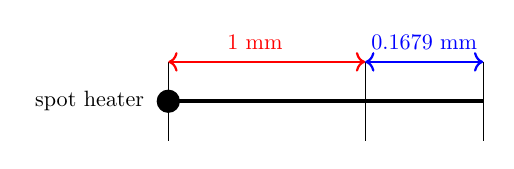
\begin{tikzpicture}[scale = 1]

\filldraw [black] (0,0) circle (4pt);
\draw [ultra thick] (0.0,0.0) -- (4.0,0);

\draw [thin] (2.5,-0.5) -- (2.5,0.5);
\draw [thin] (4.0,-0.5) -- (4.0,0.5);
\draw [thin] (0.0,-0.5) -- (0.0,0.5);

\draw [thick, <->, red] (0.0,0.5) -- (2.5,0.5);
\draw [thick, <->, blue] (2.5,0.5) -- (4.0,0.5);

\node[scale=0.8, color = black] at (-1.0,0.0) {spot heater};
\node[scale=0.8, color = red] at (1.1,0.75) {1 mm};
\node[scale=0.8, color = blue] at (3.25,0.75) {0.1679 mm};

\end{tikzpicture}
\caption{Schematic of 1D insulation modelling; simulation length as a sum of ground insulation (in red) and winding insulation (in blue) connected in series.}
\end{figure}


\clearpage

\subsection{Quench Velocity Mapping}

Quench velocity before quench detection has been estimated numerically. The magnetic field inside the magnet varies in the range of $B \in (0, 3)~\text{T}$. Therefore, 7 separate 1D analysis have been conducted in ANSYS to estimate quench velocity as a function of time and magnetic field.

\begin{figure}[ht!]
    \centering
    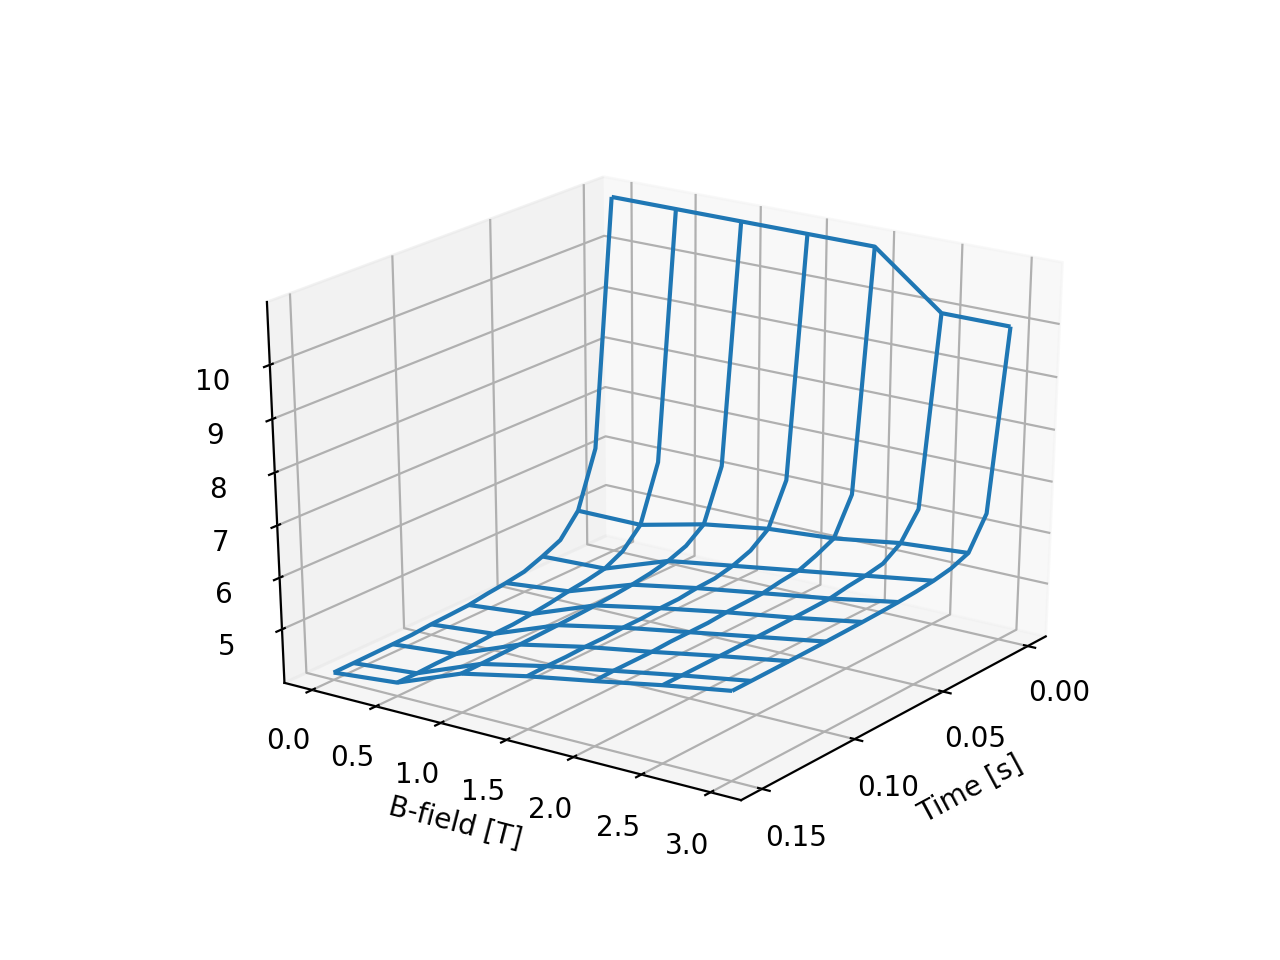
\includegraphics[width=0.6\linewidth]{figures/skew_quad_bcs/magnetic_field_mapping/Quench_Velocity_Map.png}
    \caption{Quench Velocity as a function of time and magnetic field strength}
    \label{fig:Q_v_map}
\end{figure}

\begin{figure}[H]
\centering
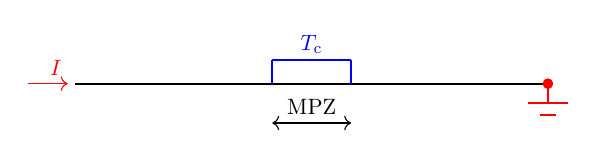
\begin{tikzpicture}[scale = 1]
\draw[thick, black] (-3,0) -- (3,0);
\filldraw[red] (3,0) circle (0.06);
\draw[thick, red] (3,0) -- (3,-0.25);
\draw[thick, red] (2.75,-0.25) -- (3.25,-0.25);
\draw[thick, red] (2.9,-0.4) -- (3.1,-0.4);
\draw[thin, red, ->] (-3.6,0) -- (-3.1,0);
\draw[thick, blue] (-0.5,0) -- (-0.5,0.3);
\draw[thick, blue] (-0.5,0.3) -- (0.5,0.3);
\draw[thick, blue] (0.5,0.3) -- (0.5,0);
\draw[thin, black, <->] (-0.5,-0.5) -- (0.5,-0.5);
\node[scale=0.8] at (0,-0.3) {MPZ};
\node[scale=0.8, blue] at (0,0.5) {$T_\text{c}$};
\node[scale=0.8, red] at (-3.25,0.2) {$I$};
\end{tikzpicture}
\caption{Simulation settings}
\label{fig:sim_settings_1}
\end{figure}

\begin{figure}[H]
\centering
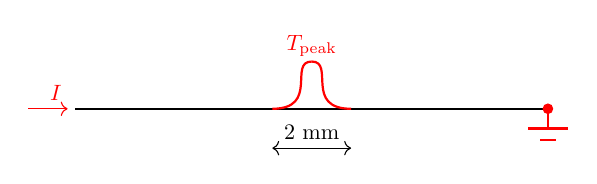
\begin{tikzpicture}[scale = 1]
\draw[thick, black] (-3,0) -- (3,0);
\filldraw[red] (3,0) circle (0.06);
\draw[thick, red] (3,0) -- (3,-0.25);
\draw[thick, red] (2.75,-0.25) -- (3.25,-0.25);
\draw[thick, red] (2.9,-0.4) -- (3.1,-0.4);
\draw[thin, red, ->] (-3.6,0) -- (-3.1,0);
\draw [thick, red] (-0.5,0) .. controls +(0:0.6cm) and +(180:0.3cm) .. (0,0.6);
\draw [thick, red] (0,0.6) .. controls +(0:0.3cm) and +(180:0.6cm) .. (0.5,0);
\draw[thin, black, <->] (-0.5,-0.5) -- (0.5,-0.5);
\node[scale=0.8] at (0,-0.3) {2 mm};
\node[scale=0.8, red] at (0,0.8) {$T_\text{peak}$};
\node[scale=0.8, red] at (-3.25,0.2) {$I$};
\end{tikzpicture}
\caption{Simulation settings}
\label{fig:sim_settings_2}
\end{figure}

\begin{figure}[H]
\centering
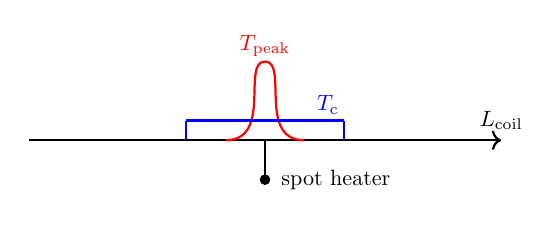
\begin{tikzpicture}[scale = 1]
\draw[thick, black, ->] (-3,0) -- (3,0);
\filldraw[black] (0,-0.5) circle (0.06);
\draw[thick, black] (0,0) -- (0,-0.5);
\draw [thick, red] (-0.5,0) .. controls +(0:0.6cm) and +(180:0.3cm) .. (0,1);
\draw [thick, red] (0,1) .. controls +(0:0.3cm) and +(180:0.6cm) .. (0.5,0);
\draw[thick, blue] (-1,0) -- (-1,0.25);
\draw[thick, blue] (-1,0.25) -- (1,0.25);
\draw[thick, blue] (1,0.25) -- (1,0);
\node[scale=0.8, black] at (0.9,-0.5) {spot heater};
\node[scale=0.8, black] at (3,0.25) {$L_\text{coil}$};
\node[scale=0.8, blue] at (0.8,0.45) {$T_\text{c}$};
\node[scale=0.8, red] at (0,1.2) {$T_\text{peak}$};
\end{tikzpicture}
\end{figure}

\begin{figure}[H]
\centering
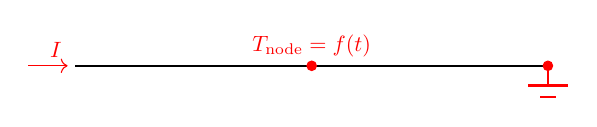
\begin{tikzpicture}[scale = 1]
\draw[thick, black] (-3,0) -- (3,0);
\filldraw[red] (3,0) circle (0.06);
\draw[thick, red] (3,0) -- (3,-0.25);
\draw[thick, red] (2.75,-0.25) -- (3.25,-0.25);
\filldraw[red] (0,0) circle (0.06);
\draw[thick, red] (2.9,-0.4) -- (3.1,-0.4);
\draw[thin, red, ->] (-3.6,0) -- (-3.1,0);
\node[scale=0.8, red] at (0,0.25) {$T_\text{node}= f(t)$};
\node[scale=0.8, red] at (-3.25,0.2) {$I$};
\end{tikzpicture}
\caption{Simulation settings}
\label{fig:sim_settings_3}
\end{figure}


% Analysis assumptions:
% No helium cooling
% Power input heats up the coil directly (no intermediate insulation layer) 
% Temperature in the windings’ cross-sectional area is uniform - 1D element
% Longitudinal heat transfer inside the insulation is negligible with respect to windings - 1D element


% Winding: 	link68, thermo-electric 1D elements for heat conduction + Joule heating
% Insulation: 	link33, thermal 1D elements for heat conduction



% Resistive voltage curve changes the slope during the analysis, - turn-to-turn propagation occurs in the model

% Turn-to-turn propagation occurs to slow compared to measurements-assumptions related to insulation elements are too conservative

% In measurements, quench spot is applied through insulation  direct power input in simulations ought to be modified

% Exact value of RRR of the measured magnet needs to be verified with INFN 


% Preparation of thermo-magneto-electric model to simulate current discharge

% Preparation of magnetic model in ANSYS to simulate magnetic field change during discharge (influence of iron yoke)
% Coupling of ANSYS quench velocity model with circuit in PSpice 
% Validation against measurements from INFN


\begin{figure}
\centering
\begin{tikzpicture}
\pgfplotsset{
    scale only axis,
    height=4cm,
    width=8cm,
    compat=1.3,
    scaled x ticks=base 10:0,
    xmin=0, xmax=9
}
\begin{axis}[
  axis y line*=left,
  ymin=0, ymax=20,
  xlabel={Time, s},
  ylabel={Resistive Voltage, V},
]
\addplot[smooth, red] table[x=Time,y=Resistive_Voltage,col sep=comma] {figures/skew_quad_bcs/current_voltage_discharge.csv}; 
\label{plot_resistive_voltage}
\end{axis}

\begin{axis}[
  axis y line*=right,
  axis x line=none,
  ymin=0, ymax=100,
  ylabel={Current, A}
]
\addplot[smooth, blue] table[x=Time,y=Current,col sep=comma] {figures/skew_quad_bcs/current_voltage_discharge.csv}; 
\label{current}
\addlegendentry{$I$}
\addlegendimage{/pgfplots/refstyle=plot_resistive_voltage}\addlegendentry{$V_\text{r}$}
\end{axis}
\end{tikzpicture}
\caption{Current and Resistive Voltage change during the discharge of skew quadrupole}
\label{fig:skew_quad_discharge}
\end{figure}


\begin{figure}
\centering
\begin{tikzpicture}
\pgfplotsset{
    scale only axis,
    height=4cm,
    width=8cm,
    compat=1.3,
    scaled x ticks=base 10:3,
    xmin=0, xmax=0.15
}
\begin{axis}[
  axis y line*=left,
  ymin=0, ymax=0.35,
  xlabel={Time, s},
  ylabel={Resistive Voltage, V},
]
\addplot[smooth, red] table[x=Time,y=Resistive_Voltage,col sep=comma] {figures/skew_quad_bcs/current_voltage_quench_detection.csv}; 
\label{plot_resistive_voltage}
\end{axis}

\begin{axis}[
  axis y line*=right,
  axis x line=none,
  ymin=0, ymax=100,
  ylabel={Current, A},
  legend pos=south east
]
\addplot[smooth, blue] table[x=Time,y=Current,col sep=comma] {figures/skew_quad_bcs/current_voltage_quench_detection.csv}; 
\label{current}
\addlegendentry{$I$}
\addlegendimage{/pgfplots/refstyle=plot_resistive_voltage}\addlegendentry{$V_\text{r}$}
\end{axis}
\end{tikzpicture}
\caption{Current and Resistive Voltage change during the discharge of skew quadrupole}
\label{fig:skew_quad_discharge}
\end{figure}

% APPENDICES
\clearpage
\begin{appendices}

\section{Material Properties}
\label{appendix_material_properties_description}

The material properties are based on an update of ROXIE database prepared at CERN \cite{material_properties_roxie}. Except for Nb-Ti specific heat capacity, NIST standards for cryogenic materials are used to describe them. Nb-Ti is defined by CUDI which is Arjan Verweij's software for Rutherford cable modelling~\cite{cudi_manual}.  

\subsection{Copper}
\label{appendix:cu_material_properties}

\subsubsection{Resistivity}
Copper resistivity depends on temperature and RRR:
\begin{equation}
    \rho_\text{N}(T, \text{RRR}) = \rho_\text{0}+\rho_\text{i}+\rho_\text{i0},
\end{equation}
\\
where:
\begin{equation}
    \rho_\text{0} = \frac{1.5553\cdot10^{-8}}{\text{RRR}}
\end{equation}

\begin{equation}
    \rho_\text{i} = \frac{\text{P}_\text{1}}{1+\text{P}_\text{1}  \text{P}_\text{3}  T^{\text{P}_\text{2} - \text{P}_\text{4}}  \exp{[-(\frac{\text{P}_\text{5}}{T}}^{\text{P}_\text{6}})]}
\end{equation}

\begin{equation}
    \rho_\text{i0} = \text{P}_\text{7} \frac{\rho_\text{i} \rho_\text{0}}{\rho_\text{i} + \rho_\text{0}}
\end{equation}
\\
In order to apply the resistivity dependence on magnetic field strength, the following formula are applied with fit parameters presented in Table \ref{table:nist_resistivity_parameters}:
\begin{equation}
    \rho_\text{N}(T, B, \text{RRR}) = \rho_\text{N}(T, \text{RRR}) \cdot (1 + 10^{a(x)}),  
\end{equation}
\\
where:
\begin{equation}
    a(x) = \sum_{n=0}^{N} a_\text{n}(\log_\text{10}x)^{n}
\end{equation}

\begin{equation}
    x \approx \frac{1.553 \cdot 10^{-8}}{\rho_\text{N}(T, \text{RRR})} \cdot B
\end{equation}

\begin{table}[h!]
    \caption{Fit parameters for NIST copper electrical resistivity} 
    \vspace{-1.em} 
    \fontsize{10}{10}
    \selectfont 
    \renewcommand{\arraystretch}{1.5}
    \begin{center}
    \begin{tabular}{ ccccccc }  
    \hline
    $\text{P}_1$ & $\text{P}_2$ & $\text{P}_3$ & $\text{P}_4$ & $\text{P}_5$ & $\text{P}_6$ & $\text{P}_7$ \\
    \hline
    $1.171\cdot10^{-17}$ & 4.49 & $3.841\cdot10^{10}$ & 1.14 & 50 & 6.428 & 0.4531 \\
    \hline 
    \end{tabular}
    \\
    \begin{tabular}{ ccccc }  
    $\text{a}_0$ & $\text{a}_1$ & $\text{a}_2$ & $\text{a}_3$ & $\text{a}_4$ \\
    \hline
    -2.662 & 0.3168 & 0.6229 & -0.1839 & 0.001827 \\
    \hline
    \end{tabular}
    \end{center}  
     \label{table:nist_resistivity_parameters} 
 \end{table}

Fig. \ref{fig:cu_resistivity_plot} shows copper resistivity for low and high value of RRR. In general, it rises with temperature, decrease of RRR and increase of magnetic field strength.

\begin{figure}
\centering
\begin{tikzpicture}
\begin{axis}[
  no markers,
  legend style={at={(1,0)},anchor=south east},
  grid style={dashed,gray!30},
  width=0.85\linewidth, 
  height = 6cm,
  xlabel={$t$},
  ylabel={$\rho_{Cu}$},
  xlabel style={below right},
  ylabel style={above left},
  xmin=0.0,
  ymin=0.0,
  xmax=100.0
  ]
  
  \addplot table[x=Time,y=B_0_0_RRR_100,col sep=comma] {figures/material_properties/Cu_Rho_B_Depenedence.csv}; 
  \addplot table[x=Time,y=B_3_0_RRR_100,col sep=comma] {figures/material_properties/Cu_Rho_B_Depenedence.csv}; 
  \addplot table[x=Time,y=B_0_0_RRR_200,col sep=comma] {figures/material_properties/Cu_Rho_B_Depenedence.csv}; 
  \addplot table[x=Time,y=B_3_0_RRR_200,col sep=comma] {figures/material_properties/Cu_Rho_B_Depenedence.csv}; 
  
  \legend{$B(\text{RRR}=100)=0~\text{T}$,
  $B(\text{RRR}=100)=3~\text{T}$,
  $B(\text{RRR}=200)=0~\text{T}$,
  $B(\text{RRR}=200)=3~\text{T}$}

\end{axis}
\end{tikzpicture}
\caption{Copper resistivity temperature dependence for varying magnetic field and RRR}
    \label{fig:cu_resistivity_plot}
\end{figure}

%  thermal conductivity
\subsubsection{Thermal Conductivity}
Copper thermal conductivity depends on temperature and RRR:
\begin{equation}
    k_\text{N}(T, \text{RRR}) = \frac{1}{\text{W}_\text{0} + \text{W}_\text{i} + \text{W}_\text{i0}}, 
\end{equation}
\\ 
where:
\begin{equation}
    \text{W}_\text{0} = \frac{\beta}{T}
\end{equation}

\begin{equation}
    \text{W}_\text{i} = \frac{\text{P}_\text{1} T^{\text{P}_\text{2}}}{1+\text{P}_\text{1}  \text{P}_\text{3}  T^{\text{P}_\text{2} + \text{P}_\text{4}}  \exp{[-(\frac{\text{P}_\text{5}}{T}}^{\text{P}_\text{6}})]}
\end{equation}

\begin{equation}
    \text{W}_\text{i0} = \text{P}_\text{7} \frac{\text{W}_\text{i} \text{W}_\text{0}}{\text{W}_\text{i} + \text{W}_\text{0}}
\end{equation}
\\
with fit parameters presented in Table \ref{table:nist_cu_k_parameters}.

\begin{table}[h!]
    \caption{Fit parameters for NIST copper thermal conductivity} 
    \vspace{-1.em} 
    \fontsize{10}{10}
    \selectfont 
    \renewcommand{\arraystretch}{1.5}
    \begin{center}
    \begin{tabular}{ cc }  
    $\beta$ & $\beta_\text{r}$ \\
    \hline
    $0.634/\text{RRR}$ & $\beta/0.0003$ \\
    \hline
    \end{tabular}
    
    \begin{tabular}{ ccccccc }  
    $\text{P}_1$ & $\text{P}_2$ & $\text{P}_3$ & $\text{P}_4$ & $\text{P}_5$ & $\text{P}_6$ & $\text{P}_7$ \\
    \hline
    $1.754\cdot10^{-8}$ & 2.763 & 1102 & -0.165 & 70 & 1.756 & $0.838/\beta_\text{r}^{0.1661}$ \\
    \hline 
    \end{tabular}
    \end{center}  
     \label{table:nist_cu_k_parameters} 
 \end{table}
 
 In order to include the magnetic induction dependence in the function of thermal conductivity, one can apply: 
\begin{equation}
    k_\text{N}(T, B, \text{RRR}) = \frac{\rho\text{N}(T, B=0, \text{RRR})}{\rho\text{N}(T, B=0, \text{RRR})} \cdot k_\text{N}(T, \text{RRR})
\end{equation}

As presented in Fig. \ref{fig:cu_k_plot}, thermal conductivity decreases with increase of magnetic field strength and when a cable is characterised by lower RRR. One can also notice that the peak value of thermal conductivity occurs at lower temperatures when RRR is high. 
 
\begin{figure}[h!]
    \centering
    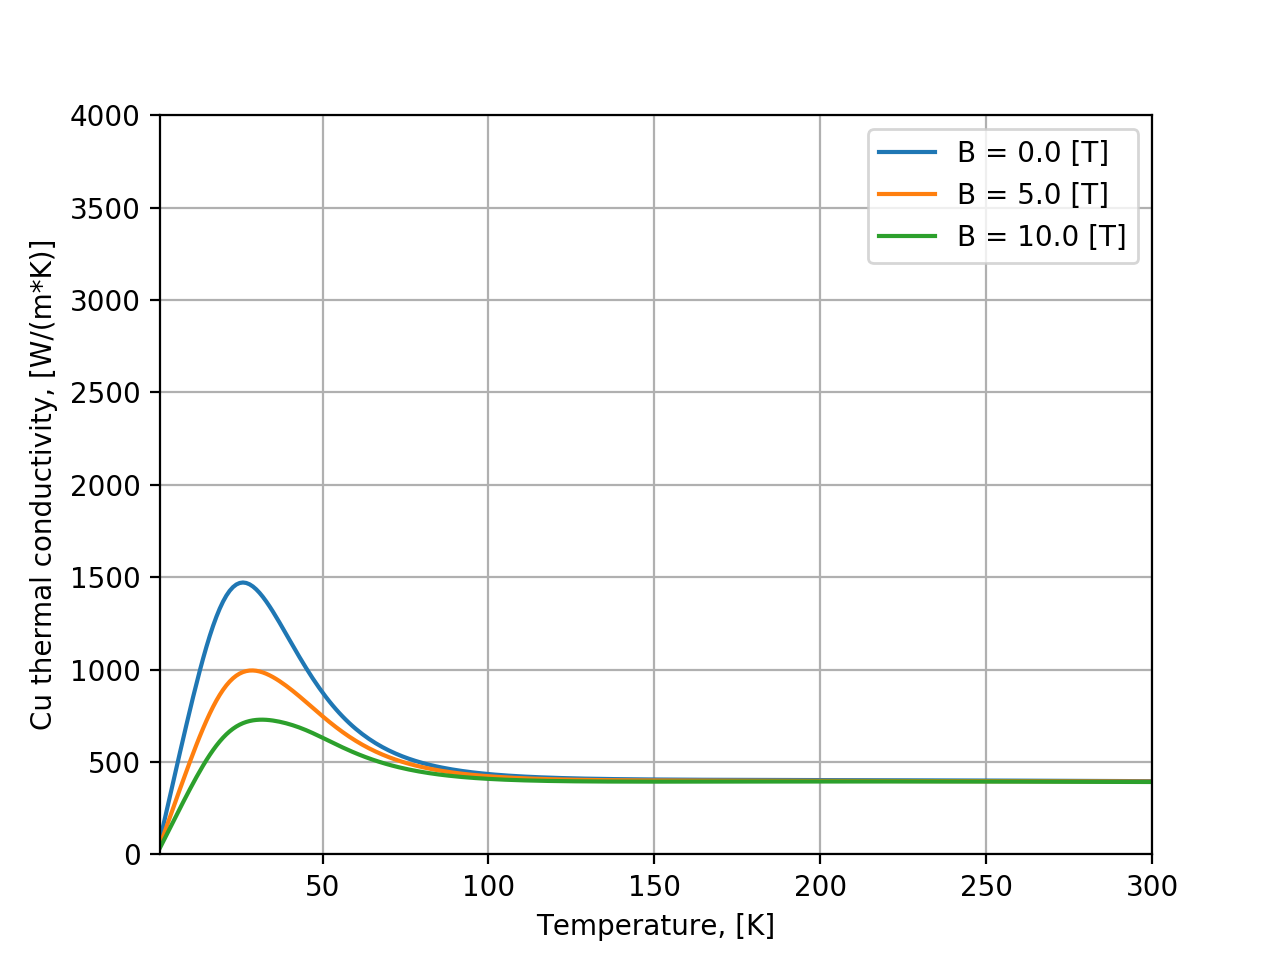
\includegraphics[width=0.49\linewidth]{figures/material_properties/Cu_k_B_Depenedence_plot_rrr_50.png}
    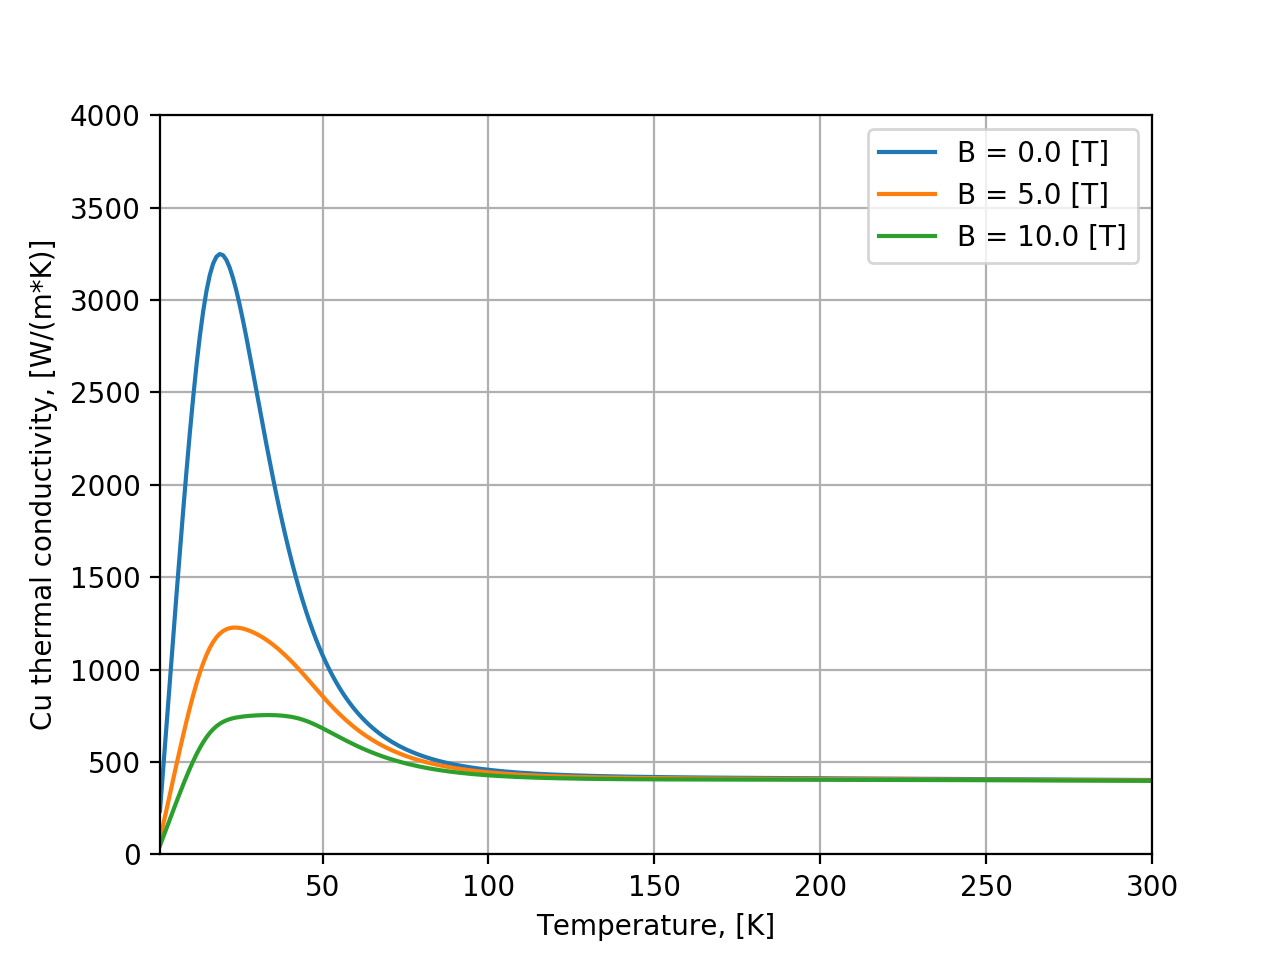
\includegraphics[width=0.49\linewidth]{figures/material_properties/Cu_k_B_Depenedence_plot_rrr_150.png}
    \caption{Copper thermal conductivity temperature dependence for three values of magnetic field for RRR = 50 (left) and RRR = 150 (right) }
    \label{fig:cu_k_plot}
\end{figure}

% mass density 
\subsubsection{Mass Density}
The mass density of copper is assumed to be constant and equal to $\rho = 8960~\text{kg/m}^{3}$.

% specific heat capacity 
\subsubsection{Specific Heat Capacity}
Copper specific heat capacity is approximated with the NIST polynomial interpolation. The fit with parameters described in Table \ref{table:nist_cu_cp_parameters}, is valid in the range between 4 and 300 K. It is assumed that the fit is valid throughout the entire analysis of quench.

\begin{equation}
    x(T) = 10^{\sum_{n=0}^{N} a_\text{n}(\log_\text{10}T)^{n}},
\end{equation}
\\
where $N$ refers to the order of polynomial.

\begin{table}[h!]
    \caption{Fit parameters for NIST copper specific heat capacity} 
    \vspace{-1.em} 
    \fontsize{10}{10}
    \selectfont 
    \renewcommand{\arraystretch}{1.5}
    \begin{center}
    \begin{tabular}{ cccccccc }  
    $\text{a}_0$ & $\text{a}_1$ & $\text{a}_2$ & $\text{a}_3$ & $\text{a}_4$ & $\text{a}_5$ & $\text{a}_6$ & $\text{a}_7$ \\
    \hline
    -1.91844 & -0.15973 & 8.61013 & -18.996 & 21.9661 & -12.7328 & 3.54322 & -0.3797 \\
    \hline 
    \end{tabular}
    \end{center}  
     \label{table:nist_cu_cp_parameters} 
 \end{table}

\begin{figure}[h!]
    \centering
    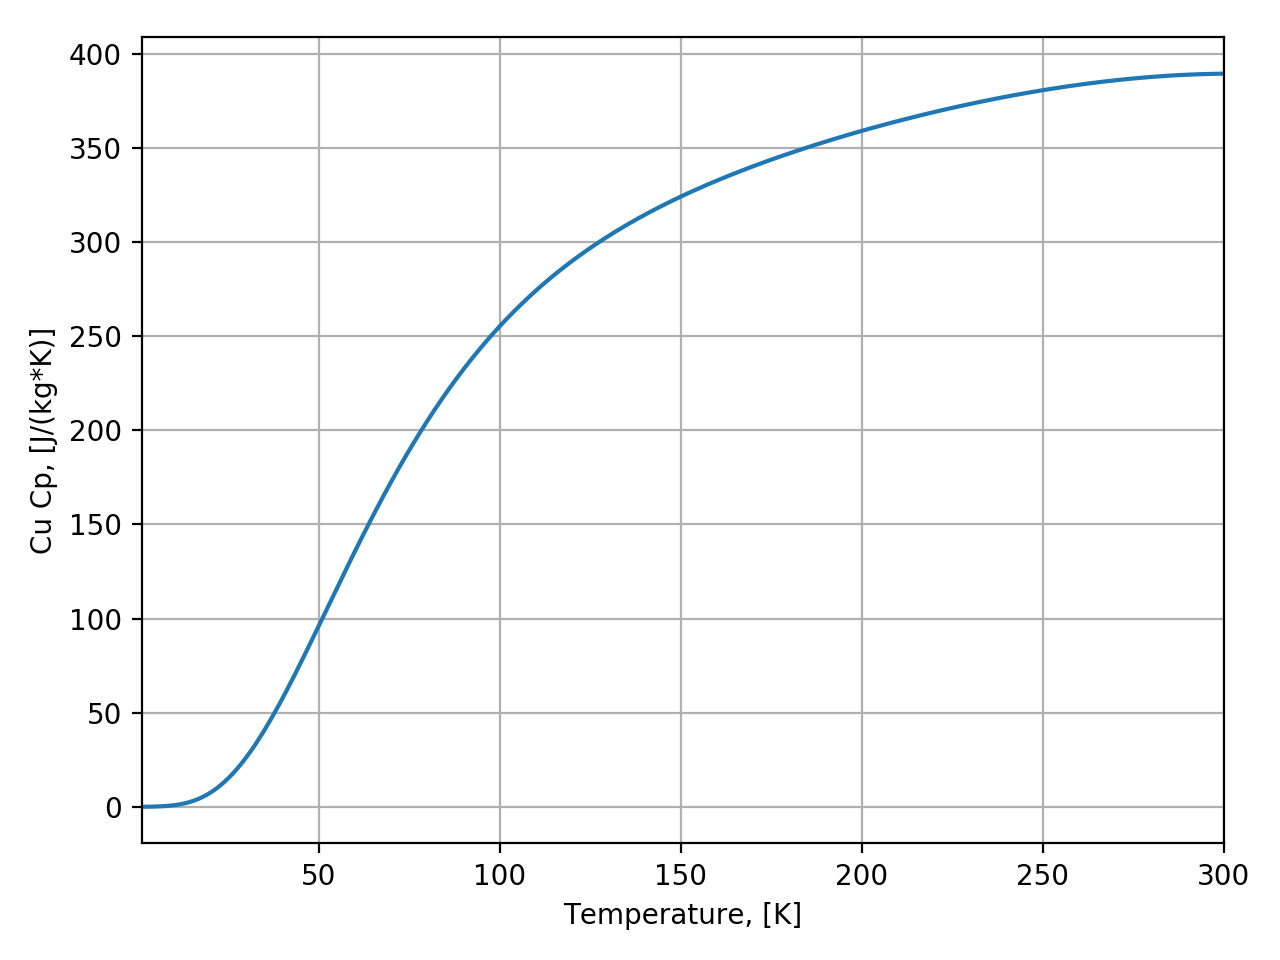
\includegraphics[width=0.49\linewidth]{figures/material_properties/Cu_Cp_plot.png}
    \caption{Copper specific heat capacity temperature dependence}
    \label{fig:cu_cp_plot}
\end{figure}
\newpage

% \subsection{Niobium Titanium}
% \label{appendix:nbti_material_properties}
% 
% NbTi mass density 
\subsubsection{Mass Density}
The mass density is assumed to be constant and equal to $\rho = 6000~\text{kg/m}^{3}$.

% NbTi specific heat capacity
\subsubsection{Specific Heat Capacity}
Volumetric heat capacity of Nb-Ti is estimated by means of a piece-wise polynomial function which takes into account a linear magnetic dependence below the critical temperature $T_\text{c}$. In order to obtain specific heat capacity in [$\frac{\text{J}}{\text{kg} \cdot \text{K}}$], the function is divided by a constant mass density. The fit parameters are presented in Table \ref{table:nbti_parameters}.

\begin{equation}
    \left\{ \begin{array}{ll}
    Cp_\text{ NbTi}(T, T_\text{c}) = \frac{\text{a}_0 + \text{a}_1\cdot T^{1} + \text{a}_2\cdot T^{2} + \text{a}_3\cdot T^{3}+ \text{a}_4\cdot T^{4}} {\rho_{Nb-Ti}} \\ \\
    T_\text{c}(B) = T_\text{c0}\cdot(1-\frac{B}{B_\text{c20}})^{0.59}
    \end{array} \right.
\end{equation}

\begin{table}[h!]
    \caption{Polynomial parameters} 
    \vspace{-1.em} 
    \fontsize{10}{10}
    \selectfont 
    \renewcommand{\arraystretch}{1.5}
    \begin{center}
    \begin{tabular}{ lccccc }  
    \hline
    & $\text{a}_0$ & $\text{a}_1$ & $\text{a}_2$ & $\text{a}_3$ & $\text{a}_4$ \\
    \hline
    $T \in (0, T_\text{c})$~K & 0 & $64 \cdot B$ & 0 & 49.1 & 0 \\        
    $T \in [T_\text{c}, 28.358)$~K & 0 & 928 & 0 & 16.24 & 0 \\        
    $T \in [28.358, 50.99)$~K & 41383 & -7846.1 & 553.71 & 11.9838 & -0.2177 \\        
    $T \in [50.99, 165.8)$~K & $-1.53\cdot10^{6}$ & 83022 & -716.3 & 2.976 & -0.00482 \\ 
    $T \in [165.8, 496.54)$~K & $1.24\cdot10^{6}$ & 13706 & -51.66 & 0.09296 & $-6.29\cdot10^{-5}$ \\        
    $T \in [496.54, 1000)$~K & $2.45\cdot10^{6}$ & 955.5 & -0.257 & 0 & 0 \\       
    \hline
     \end{tabular} 
    \end{center}  
     \label{table:nbti_parameters} 
 \end{table}
 
 \begin{figure}[h!]
    \centering
    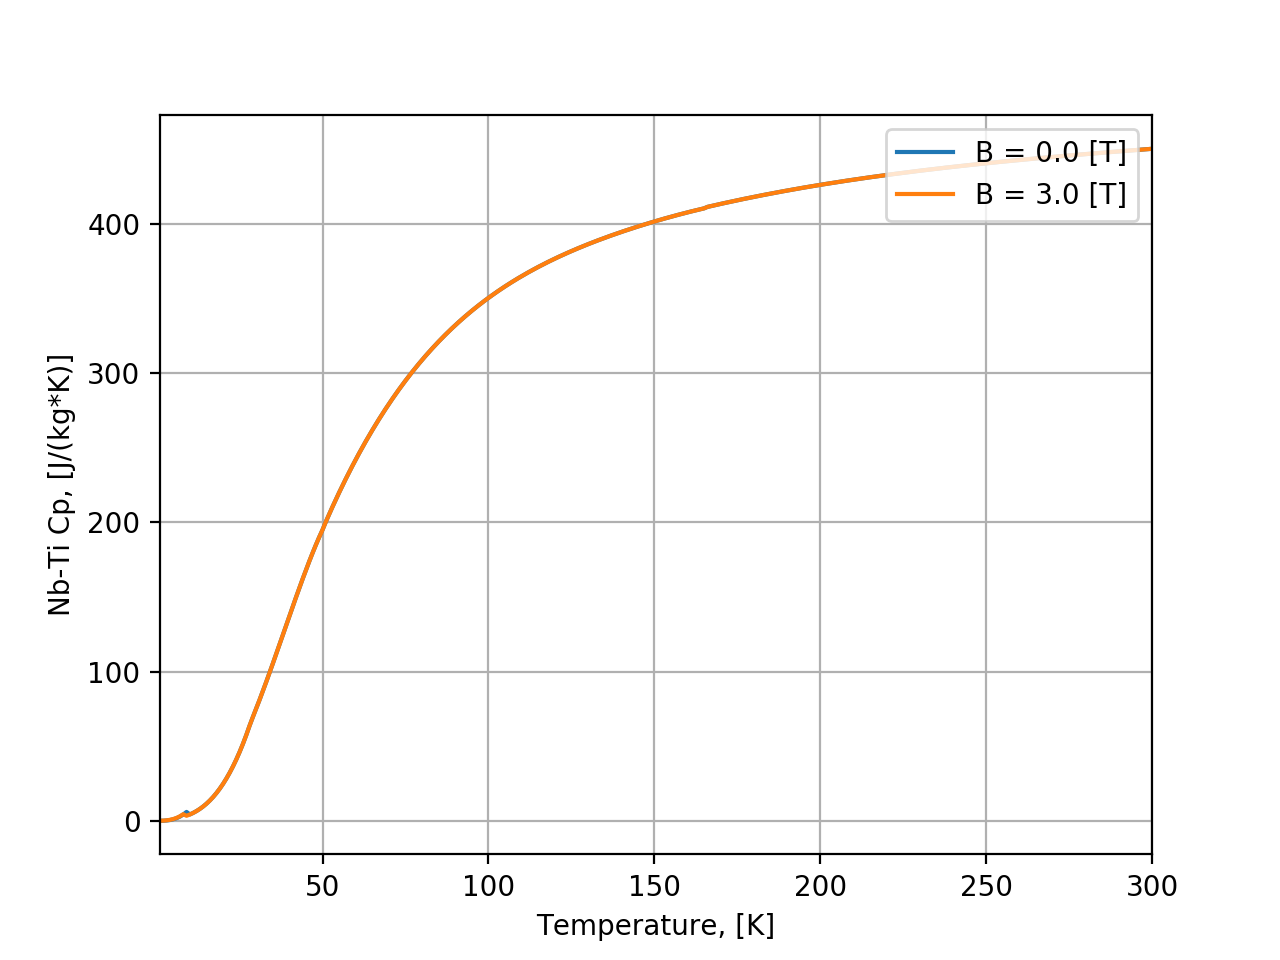
\includegraphics[width=0.49\linewidth]{figures/material_properties/NbTi_Cp_B_Depenedence_plot.png}
    \caption{Nb-Ti specific heat capacity temperature dependence for two values of magnetic field}
    \label{fig:nbti_cp_plot}
\end{figure}
\newpage


% \subsection{G10 Material Properties}
% \label{appendix:g10_material_properties}
% 
% thermal conductivity
\subsubsection{Thermal Conductivity}
G10 is an epoxy-impregnated fiberglass, thermally anisotropic. It means that its thermal conductivity along the fibers is higher than across them. In order to simplify computation in the scope of this thesis, the material is assumed to be isotropic. A conservative assumption is made which states that thermal conductivity of G10 in all directions is equal to the one normal to the direction of the fibers.
G10 thermal conductivity as well as specific heat capacity is approximated with the NIST polynomial interpolation:
\begin{equation}
    x(T) = 10^{\sum_{n=0}^{N} a_\text{n}(\log_\text{10}T)^{n}},
\end{equation}
\\
where $N$ refers to the order of polynomial and $x(T)$ is the considered material property. Fig. \ref{fig:g10_k_plot} presents G10 heat conductivity based on polynomial fit parameters depicted in Table \ref{table:nist_g10_k_parameters}.

\begin{table}[h!]
    \caption{Fit parameters for NIST G10 thermal conductivity} 
    \vspace{-1.em} 
    \fontsize{10}{10}
    \selectfont 
    \renewcommand{\arraystretch}{1.5}
    \begin{center}
    \begin{tabular}{ ccccccccc }  
    $\text{a}_0$ & $\text{a}_1$ & $\text{a}_2$ & $\text{a}_3$ & $\text{a}_4$ & $\text{a}_5$ & $\text{a}_6$ & $\text{a}_7$ & $\text{a}_8$ \\
    \hline
    -4.1236 & 13.788 & -26.068 & 26.272 & -14.663 & 4.4954 & -0.6905 & 0.0397 & 0 \\
    \hline 
    \end{tabular}
    \end{center}  
     \label{table:nist_g10_k_parameters} 
 \end{table}
 
  \begin{figure}[h!]
    \centering
    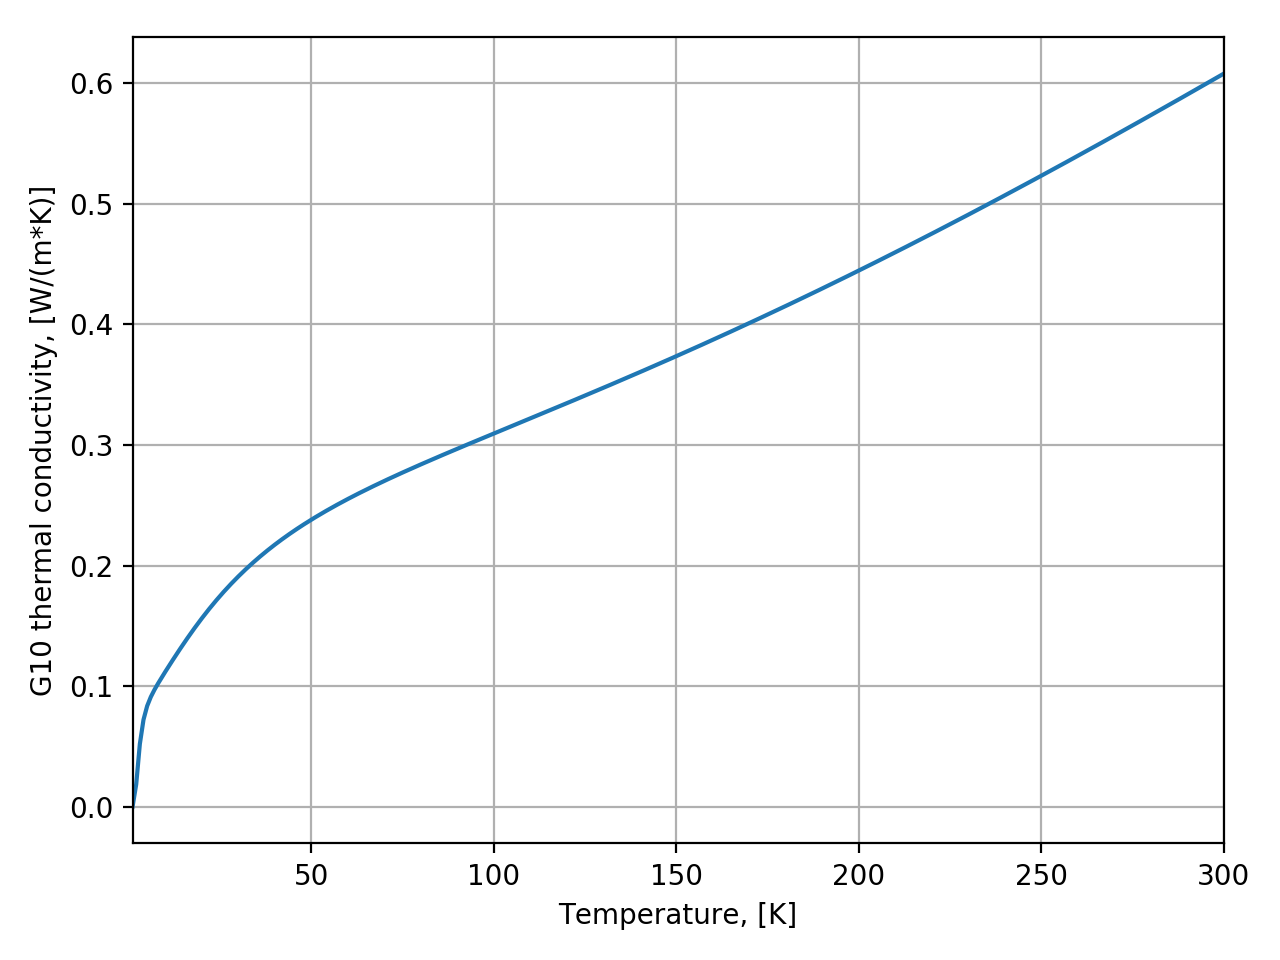
\includegraphics[width=0.49\linewidth]{figures/material_properties/G10_k_plot.png}
    \caption{G10 heat conductivity temperature dependence}
    \label{fig:g10_k_plot}
\end{figure}
 
% mass density
 \subsubsection{Mass Density}
 The mass density is assumed to be constant and equal to $\rho = 1948~\text{kg/m}^{3}$ according to NIST standards.

% specific heat capacity
\subsubsection{Specific Heat Capacity}
Fig. \ref{fig:g10_cp_plot} presents G10 specific heat capacity function based on polynomial fit parameters depicted in Table \ref{table:nist_g10_cp_parameters}.

\begin{table}[h!]
    \caption{Fit parameters for NIST G10 specific heat capacity} 
    \vspace{-1.em} 
    \fontsize{10}{10}
    \selectfont 
    \renewcommand{\arraystretch}{1.5}
    \begin{center}
    \begin{tabular}{ cccccccc }  
    $\text{a}_0$ & $\text{a}_1$ & $\text{a}_2$ & $\text{a}_3$ & $\text{a}_4$ & $\text{a}_5$ & $\text{a}_6$ & $\text{a}_7$ \\
    \hline
    -2.4083 & 7.6006 & -8.2982 & 7.3301 & -4.2386 & 1.4294 & -0.24396 & 0.015236 \\
    \hline 
    \end{tabular}
    \end{center}  
     \label{table:nist_g10_cp_parameters} 
 \end{table}

 \begin{figure}[h!]
    \centering
    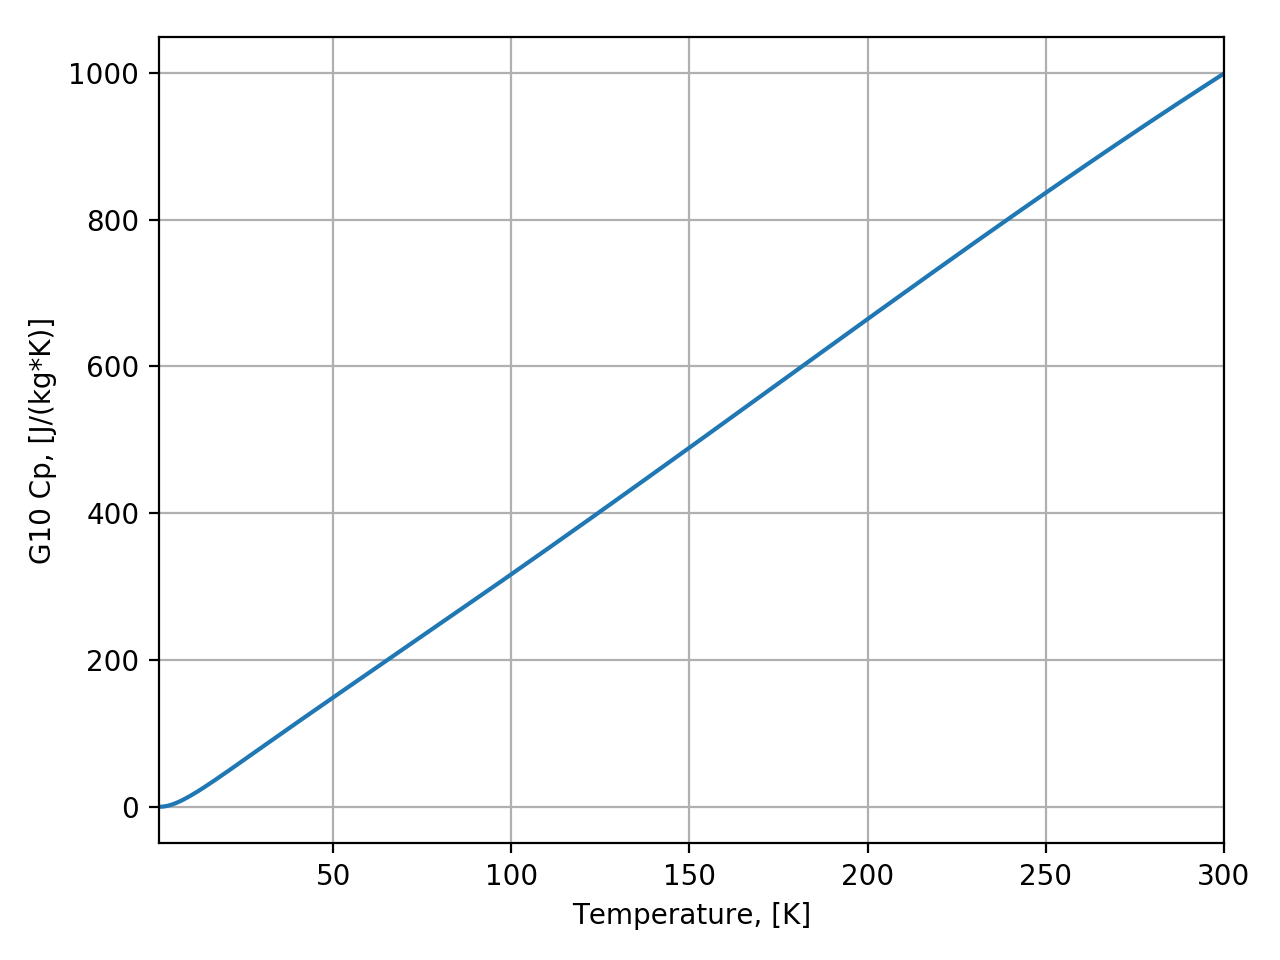
\includegraphics[width=0.49\linewidth]{figures/material_properties/G10_Cp_plot.png}
    \caption{G10 specific heat capacity temperature dependence}
    \label{fig:g10_cp_plot}
\end{figure}

\section{Compilation of ANSYS with Python Environment}
\label{appendix:python_ansys_compilation}

The representative code for Python compilation with ANSYS environment is presented in Table~\ref{table:ansys_python_compilation}.

\begin{table}[h!]
    \caption{Compilation of Python with ANSYS environment} 
    \vspace{-1em} 
    \fontsize{10}{10}
    \selectfont 
    \renewcommand{\arraystretch}{1}
    \begin{center}
    \begin{tabular}{ ll }  
    \hline  
        from ansys\_corba import CORBA & - imports ANSYS library \\
        os.chdir(directory) & - sets analysis directory\\
        with open('aaS\_MapdlID.txt', 'r') as f: \\ aasMapdlKey = f.read() & - opens APDL analysis \\
        mapdl = CORBA.ORB\_init().string\_to\_object(aasMapdlKey) & - creates mapdl object \\
    \hline
        mapdl.executeCommandToString("/prep7") & - exemplary command \\
     \end{tabular} 
    \end{center}  
     \label{table:ansys_python_compilation} 
 \end{table}
\newpage

% \section{Mapping Algorithm Python Script}
% \section{Quench Velocity Algorithm Python Script}
% \section{Nodes Search Algorithm Python Script}

\end{appendices}

\clearpage
\bibliographystyle{IEEEtran}
\bibliography{IEEEabrv,./bib/article}

\end{document}
